% =============================================================================
% SimForge thesis — main LaTeX entry point
%
% Title: SimForge: A Reproducible Cross-Simulator Testing Framework for Urban
%        Mobility Simulation
% Author: Phanidhar Akula
% Year:   2026
%
% Build:  see latex/README.md for Overleaf upload + local compile instructions.
%
% This file deliberately uses a clean academic template (report class +
% biblatex + biber). If your school requires a specific template (OSU has
% one), replace this file with the school's template + \include the same
% chapter files from latex/chapters/.
% =============================================================================

\documentclass[12pt,letterpaper,oneside]{report}

% ---- Geometry: 1.5" left binding margin, 1" elsewhere (OSU convention) ----
\usepackage[left=1.5in,right=1in,top=1in,bottom=1in]{geometry}

% ---- Fonts: Times New Roman family (newtxtext + newtxmath) ----
\usepackage{newtxtext,newtxmath}

% ---- Double-spaced body, single-spaced for verbatim/code ----
\usepackage{setspace}
\doublespacing

% ---- Graphics + figures ----
\usepackage{graphicx}
\graphicspath{{figures/}{../figures/}}
\usepackage{float}

% ---- Tables ----
\usepackage{booktabs}
\usepackage{longtable}
\usepackage{array}
\usepackage{tabularx}

% ---- Math + symbols ----
\usepackage{amsmath,amssymb}

% ---- Code listings (verbatim with line wrapping) ----
\usepackage{listings}
\lstset{
  basicstyle=\ttfamily\small,
  breaklines=true,
  breakatwhitespace=true,
  frame=single,
  showstringspaces=false,
  numbers=left,
  numberstyle=\tiny\color{gray},
}

% ---- Hyperlinks + cross-references (load last to be safe) ----
\usepackage[colorlinks=true,linkcolor=black,urlcolor=blue,citecolor=blue]{hyperref}
\usepackage{xcolor}

% ---- Bibliography: biblatex with biber backend ----
\usepackage[backend=biber,style=authoryear,sorting=nyt,maxcitenames=2,minbibnames=10,giveninits=true]{biblatex}
\addbibresource{references.bib}

% ---- Pandoc helpers (some chapters use \pandocbounded, tightlist, etc.) ----
\usepackage{calc}
\providecommand{\pandocbounded}[1]{#1}
\providecommand{\tightlist}{}

% ---- Title metadata ----
\title{SimForge: A Reproducible Cross-Simulator Testing Framework for Urban Mobility Simulation}
\author{Phanidhar Akula}
\date{2026}

\begin{document}

% =============================================================================
% FRONT MATTER (roman numerals)
% =============================================================================
\frontmatter
\pagenumbering{roman}

% =============================================================================
% Title page — clean academic template; replace with school's official one
% if required (OSU graduate school provides a .cls/.sty for thesis title pages).
% =============================================================================

\begin{titlepage}
\centering

\vspace*{1in}

{\Large \bfseries SimForge: A Reproducible Cross-Simulator Testing Framework for Urban Mobility Simulation \par}

\vspace{1.5in}

A Thesis Presented in Partial Fulfillment of the Requirements for the Degree

\vspace{0.3in}

\textbf{[FILL: Master of Science / Master of Engineering / ...]}

\vspace{0.3in}

in the Graduate School of \textbf{[FILL: school name]}

\vspace{1in}

By

\vspace{0.3in}

{\large \bfseries Phanidhar Akula\par}

\vspace{0.3in}

Graduate Program in \textbf{[FILL: program name -- e.g., Computer Science and Engineering]}

\vspace{1in}

\textbf{[FILL: University name]}

\vspace{0.3in}

2026

\vspace{1in}

Thesis Committee:

\vspace{0.2in}

\begin{tabular}{l}
\textbf{[FILL: Advisor name]}, Advisor \\
\textbf{[FILL: Committee member 2]} \\
\textbf{[FILL: Committee member 3]} \textit{(if required)} \\
\end{tabular}

\end{titlepage}

\thispagestyle{empty}
\vspace*{\fill}
\begin{center}
Copyright by \\[0.5em]
\textbf{Phanidhar Akula} \\[0.5em]
2026
\end{center}
\vspace{0.3in}
\begin{center}
\footnotesize
SimForge software released under the Apache License 2.0. \\
Canonical scenario bundles released under CC BY 4.0 + ODbL (share-alike on OSM-derived networks). \\
Pinned-digest container image: \texttt{ghcr.io/phanidharakula/simforge:db8d786}. \\
Thesis document: \textbf{[FILL: thesis copyright -- typically all rights reserved; or CC BY 4.0 if you opt for open access]}.
\end{center}
\vspace*{\fill}
\clearpage

% =============================================================================
% Dedication — plan-style: \section*{} with \addcontentsline + \phantomsection
% =============================================================================

\clearpage
\thispagestyle{plain}
\section*{Dedication}
\phantomsection
\addcontentsline{toc}{section}{Dedication}

\vspace{2in}

\begin{center}
\textit{To \textbf{[FILL: e.g., my parents, my advisor, ...]}}
\end{center}

\clearpage

\chapter*{Acknowledgments}
\addcontentsline{toc}{chapter}{Acknowledgments}

I am deeply grateful to my advisor, \textbf{[FILL: advisor name]}, for \textbf{[FILL: 1--2 specific things the advisor did that mattered most -- e.g., introducing me to cross-simulator benchmarking as a research direction; tolerating $\sim$14 iterations on the canonical schema design; making time for weekly check-ins through the Phase 14 engineering crunch]}.

I thank my thesis committee members \textbf{[FILL: name 2]} and \textbf{[FILL: name 3]} for \textbf{[FILL: e.g., their feedback on the plan draft, their patience during the engine roster pivot from LPSim/POLARIS to DTALite]}.

This work would not have been possible without the open-source software it builds on. I acknowledge the developers of \textbf{SUMO} (Eclipse Foundation, originating at DLR Berlin); \textbf{MATSim} (ETH Z\"urich + TU Berlin community); \textbf{DTALite} (originally Arizona State University, distributed via \texttt{path4gmns}); and the \textbf{cityscape} activity-based population synthesizer developed by Prof.\ Dhananjai M.\ Rao's research group at Miami University, whose ModelGen output is the substrate for every SimForge demand bundle.

I thank the \textbf{Ohio Supercomputer Center} (OSC) for compute time on the Pitzer and Cardinal clusters under allocation \texttt{PMIU0110}. The 639-test suite and the 200K + 500K tier benchmarks would have been infeasible without HPC access. Specific thanks to \textbf{[FILL: any OSC staff who helped, or omit this paragraph]} for \textbf{[FILL: troubleshooting, allocation extensions, etc.]}.

The pinned-digest container distribution (Wave 2) builds on the \textbf{GitHub Container Registry} + \textbf{GitHub Actions} infrastructure provided free of charge to public repositories. The visualization component depends on data from the \textbf{U.S.\ Census Bureau} (PUMS, TIGER/Line), the \textbf{Oak Ridge National Laboratory} (LandScan), \textbf{IPUMS USA} (PUMA shapefiles), and \textbf{OpenStreetMap contributors} (road and building geometry under ODbL share-alike).

\textbf{[FILL: optional -- colleagues / labmates / friends who provided specific feedback, e.g., ``I thank X for the careful read of the \S5.6.3 cross-platform-reproducibility narrative that caught the JVM-build attribution error'' -- be specific where possible]}.

Finally, thanks to \textbf{[FILL: family / partner / personal support people]} for \textbf{[FILL: their patience during the multi-week thesis-writing crunch / etc.]}.

\clearpage

\clearpage
\thispagestyle{plain}
\section*{Abstract}
\phantomsection
\addcontentsline{toc}{section}{Abstract}

Urban-mobility simulators inform high-stakes infrastructure decisions in
transportation planning, congestion management, and policy evaluation,
yet a foundational methodological gap persists: cross- simulator results
are not directly comparable because each simulator uses different input
formats, different execution conventions, and different metric
definitions. A 10 \% difference in mean travel time between two
simulators on a nominally identical scenario could reflect genuine
paradigm-level disagreement or any of several input-interpretation,
configuration-tuning, version-pinning, floating-point, threading, and
platform-binary effects. Practitioners who must choose a simulator for
an actual planning decision have no operational way to distinguish
these.

This thesis presents \textbf{SimForge}, a reproducible cross-simulator
testing framework for urban mobility simulation that closes this gap
through four contributions: (C1) a canonical, simulator-agnostic input
bundle with field-level validation; (C2) byte-deterministic adapters for
SUMO, MATSim, and DTALite that translate the canonical bundle into each
engine\textquotesingle s native input format and apply a shared
strongly-connected-component + feasibility filter; (C3) a pinned-digest
container image (\texttt{ghcr.io/phanidharakula/simforge}) published to
GitHub Container Registry via an automated GitHub Actions workflow,
providing bit-identical reproducibility across machines; and (C4) a
programmatic cross-engine fairness audit that verifies byte-identical
feasibility verdicts (Q1), byte-identical SCC networks (Q2), identical
simulated trip-count targets (Q3), and a cross-engine mean travel-time
comparison (Q4), together with a reproducibility index R = 1 − σ/μ and
95 \% confidence intervals on every reported mean.

The framework integrates three simulator paradigms (microscopic queue
via SUMO, activity-based queue via MATSim, user-equilibrium dynamic
traffic assignment via DTALite) and is benchmarked across three U.S.
metropolitan networks (Chicago, New York City, Los Angeles) at demand
tiers from 1 K to 500 K trips per scenario. The fairness audit (Q1-Q3)
PASSes at every shipped tier, empirically demonstrating that the
canonical-input + deterministic-adapter design isolates engine-paradigm
differences from input-interpretation differences.

Four empirical findings emerged from the build and contribute to the
cross-simulator benchmarking literature beyond the original framework
deliverables. First, a shared canonical-routes BFS module (Phase 14)
reduced the chicago\_200k\_car benchmark wall by approximately 20 ×
cold-vs-cold (from 141.87 h to 7.14 h on OSC Cardinal) and 228 × for
warm-cache re-runs, making the 500 K-trip tier (nyc\_500k\_car)
tractable for the first time (12 h 8 min wall vs an \textasciitilde600 h
pre-Phase-14 projection). Second, the SUMO ↔ MATSim mean travel-time
ratio is regime-dependent: small-tier convergence (within ±5 \% at 50 K
trips) sharply reverses at saturation, reaching a 96.3 \% gap at 500 K
trips on NYC\textquotesingle s bridge-and-corridor topology, where
SUMO\textquotesingle s insertion-refusal model and
MATSim\textquotesingle s queue-hold model engage divergent
paradigm-level behaviors that the fairness contract makes attributable
to mobsim choice rather than input asymmetry. Third, at a fixed code
version the framework is bit-identical across every measured platform:
20/20 cells byte-identical between Cardinal x86\_64 host venv and
Cardinal x86\_64 container (different OS, JDK distribution, and JDK
major version); Mac arm64 ↔ Cardinal x86\_64 agreement to 4 sig figs on
mean travel time. The 0.2-3 \% per-engine shifts originally observed in
cross-platform comparisons are attributable to code-version drift
between time-separated measurements (Phase 12 ↔ Phase 14.13
routing-layer changes), not to floating-point hardware differences. The
pinned-digest container is therefore load-bearing because it freezes the
code + bundle + toolchain at a precise git SHA, not because it closes
any cross-platform numerical gap. Fourth --- sibling to the second
finding in mechanism but orthogonal in axis --- the within-engine SUMO
micro vs meso mean-TT gap \emph{narrows} at saturation (from +27 \% at 1
K trips to +7.8 \% at 200 K) while the wall-time premium grows
monotonically (1.65 × → 9 × → \textasciitilde124 ×). At saturation, both
mobsim resolutions become bound by the same insertion-refusal dynamics
that drive the cross-engine divergence; lane-level dynamics that micro
adds become second-order to the bottleneck behavior. Two paradigm-spread
phenomena (cross-engine, within-engine) thus emerge from the same
underlying mechanism, surfaced cleanly only because the fairness
contract holds.

SimForge is open-source under the Apache License 2.0 and available at
\texttt{github.com/PhanidharAkula/SimForge}. The framework, the
canonical bundles, the audit tooling, and the pinned-digest container
are intended as a foundation for future cross-simulator research that
can build on a bit-reproducible benchmark target rather than re-deriving
fairness from scratch for each comparison.

\textbf{Keywords:} urban mobility simulation, cross-simulator
benchmarking, reproducibility, SUMO, MATSim, DTALite, dynamic traffic
assignment, agent-based simulation, container reproducibility,
scientific computing.


% Table of contents + list of figures + list of tables
\renewcommand{\contentsname}{Table of Contents}
\tableofcontents
\clearpage
\listoffigures
\clearpage
\listoftables
\clearpage

% =============================================================================
% BODY MATTER (arabic numerals)
% =============================================================================
\mainmatter
\pagenumbering{arabic}

\chapter{Introduction}\label{chapter-1-introduction}

\section{Overview}\label{10-overview}

This chapter motivates the design of SimForge, a reproducible
cross-simulator testing framework for urban mobility simulation. It
opens with the practical importance of traffic-simulation outputs in
transportation planning and policy, surveys the structural barriers that
have prevented fair cross-simulator comparison to date, declares the
research questions the thesis answers, summarizes the contributions, and
outlines how the remaining chapters are organized.

The central premise: although individual urban-mobility simulators
(SUMO, MATSim, DTALite, and others) are mature, the question
\emph{"which simulator should I trust for this planning decision?"} has
no defensible answer without a framework that runs them under identical
inputs, identical execution policies, and a programmatic audit that
verifies fairness. SimForge provides that framework, and the empirical
findings that emerged from building it are themselves contributions to
the cross-simulator benchmarking literature.

\begin{center}\rule{0.5\linewidth}{0.5pt}\end{center}

\section{Motivation}\label{11-motivation}

Urban transportation simulation is the empirical backbone of modern
infrastructure planning. Departments of transportation, regional
planning organizations, and academic research groups use traffic
microsimulation and mesoscopic flow models to evaluate congestion-
pricing schemes, infrastructure investments, traffic-signal-
coordination strategies, transit-priority interventions, and
emergency-evacuation plans. The simulators that produce these
evaluations --- SUMO (Eclipse, 2002--present), MATSim (ETH Zürich

\begin{itemize}
\tightlist
\item
  TU Berlin, 2008--present), POLARIS (Argonne National Laboratory,
  2014--present), DTALite (Arizona State University, 2010--present), and
  others --- each represent decades of accumulated modeling expertise,
  calibration practice, and operational tooling.
\end{itemize}

Despite this maturity, a foundational methodological problem remains:
\emph{which simulator\textquotesingle s output should a practitioner
trust on a given scenario?} Each simulator embodies different modeling
assumptions, uses different input formats, runs under different
execution conventions, and reports different metric definitions. A 10 \%
difference in mean travel time between SUMO and MATSim on the same
nominal scenario could plausibly reflect:

\begin{enumerate}
\def\labelenumi{\arabic{enumi}.}
\tightlist
\item
  A genuine paradigm-level modeling disagreement,
\item
  A subtle difference in how each engine interpreted the input,
\item
  A difference in how each engine\textquotesingle s developer tuned
  defaults,
\item
  A non-deterministic floating-point or threading effect,
\item
  An undocumented version mismatch between two installations.
\end{enumerate}

Practitioners who must choose a tool for an actual planning decision
have no operational way to distinguish (1) from (2)-(5), because the
published cross-simulator comparison literature does not typically
isolate them. The decision becomes a function of which simulator the
practitioner is already familiar with, which is not the basis on which
infrastructure investments worth billions of dollars per year should be
made.

The methodological gap is well-documented. Surveys of agent-based
transportation modeling have flagged it consistently \cite{bazzan2014review}; computational-reproducibility studies in adjacent
fields (machine learning \cite{pineau2021reproducibility}, computational biology
\cite{goodman2016reproducibility}) have identified the same pattern of
version-pinning insufficiency that this thesis measures empirically for
transportation simulation in Chapter 5 §5.6.3. The MLPerf benchmark
suite has demonstrated in machine learning that standardized cross-tool
benchmarks accelerate field progress; no equivalent framework existed
for urban-mobility simulation at the time the plan for this thesis
was submitted (December 2025).

\begin{center}\rule{0.5\linewidth}{0.5pt}\end{center}

\section{Problem statement}\label{12-problem-statement}

The central problem this thesis addresses is the absence of an
\emph{open, reproducible, simulator-neutral framework} that enables fair
cross-simulator comparison for urban-mobility simulation under
controlled, hash-pinned, hardware-normalized conditions. More
specifically:

\begin{enumerate}
\def\labelenumi{\arabic{enumi}.}
\item
  \textbf{No canonical input bundle.} Each simulator (SUMO, MATSim,
  DTALite, ...) consumes its own native input format (\texttt{.net.xml}
  + \texttt{.rou.xml} for SUMO; \texttt{network.xml} +
  \texttt{plans.xml} for MATSim; GMNS-format CSVs for DTALite). A
  cross-simulator comparison that does not normalize the input layer
  cannot distinguish input-interpretation differences from
  engine-behavior differences.
\item
  \textbf{No deterministic adapter chain.} Each simulator has its own
  sources of non-determinism (random seeds, thread scheduling,
  floating-point ordering). Without explicit deterministic-execution
  wrappers, repeated runs of the same simulator on the same input can
  produce different outputs, and the cross-simulator comparison becomes
  a comparison of distributions rather than of paradigms.
\item
  \textbf{No programmatic fairness audit.} Even when canonical inputs
  and deterministic adapters are in place, a reader of cross- simulator
  results has no way to verify the fairness claim without inspecting
  each engine\textquotesingle s input files manually. A
  machine-checkable audit is required.
\item
  \textbf{No pinned-digest execution environment.} Even with all of the
  above in place, the engines themselves depend on platform-specific
  binaries (SUMO is compiled per-OS; MATSim runs on a JVM whose build
  affects floating-point output; DTALite\textquotesingle s bundled
  binary uses an OpenMP runtime whose version affects parallel-reduction
  ordering). Without a pinned-digest container, "same version" does not
  guarantee "same output", and the cross-simulator benchmark becomes
  platform-bound rather than algorithm-bound.
\end{enumerate}

The thesis problem is therefore: \textbf{build a framework that closes
all four gaps}, then use it to make empirical measurements that
demonstrate the framework\textquotesingle s claims and surface findings
the framework makes newly visible.

\begin{center}\rule{0.5\linewidth}{0.5pt}\end{center}

\section{Research questions}\label{13-research-questions}

The thesis is structured around four research questions, restated from
the original December 2025 plan §1.12 and refined as the work
progressed:

\textbf{RQ1 (Fidelity).} Under identical canonical inputs and identical
execution policies, how closely do different simulation engines
reproduce \emph{each other\textquotesingle s} outputs on the same
scenario? The plan originally posed this question against
observed-baseline data (RMSE, GEH, KS vs sensor measurements). As
discussed in Chapter 6 §6.4.1, the shipped framework substitutes
\emph{inter-engine} fidelity (Chapter 5 §5.3, §5.6.2) for
fidelity-vs-reality, because the observed-baseline data integration was
scoped out for compute budget reasons.

\textbf{RQ2 (Scalability).} How does engine runtime scale with agent
count, network size, and execution-context (host venv vs pinned-digest
container), once normalized per-core? The plan also asked for
per-watt normalization; this was dropped because HPC environments do not
expose live power meters at the job allocation level. Chapter 5 §5.1 and
§5.5, and Chapter 6 §6.2.1 report the scalability results.

\textbf{RQ3 (Reproducibility).} Under fixed seeds, deterministic
adapters, and pinned-digest containers, what level of run-to-run output
variance remains? The thesis measures R = 1 − σ/μ on travel-time means
across repeated runs (Chapter 5 §5.2). The shipped framework achieves R
= 1.0000 for MATSim and DTALite within a fixed execution context, and R
≥ 0.95 for SUMO across all shipped cells. A novel sub-finding (Chapter 5
§5.6.3, Chapter 6 §6.2.3): at fixed code, the framework is bit-identical
across every measured platform; the 0.2-3 \% shifts originally reported
in cross-platform comparisons are code-version drift, not platform
drift.

\textbf{RQ4 (Trade-offs).} What fidelity-throughput-paradigm trade-offs
emerge across simulators, and are these trade-offs stable across urban
topologies, congestion regimes, and computational architectures? Chapter
5 §5.4 (micro vs meso within SUMO) and §5.6.2 (meso vs meso across SUMO
and MATSim at saturation density) report two distinct trade-off regimes.
The cross-engine ratio is shown to be regime-dependent, not
regime-stable, and the saturation regime is where the paradigm signal
becomes sharpest.

\begin{center}\rule{0.5\linewidth}{0.5pt}\end{center}

\section{Contributions}\label{14-contributions}

This thesis delivers four principal contributions, corresponding to the
plan\textquotesingle s §1.11 C1-C4, and surfaces four empirical
findings that emerged during the build and form part of the
framework\textquotesingle s contribution beyond the original C-row list.

\pandocbounded{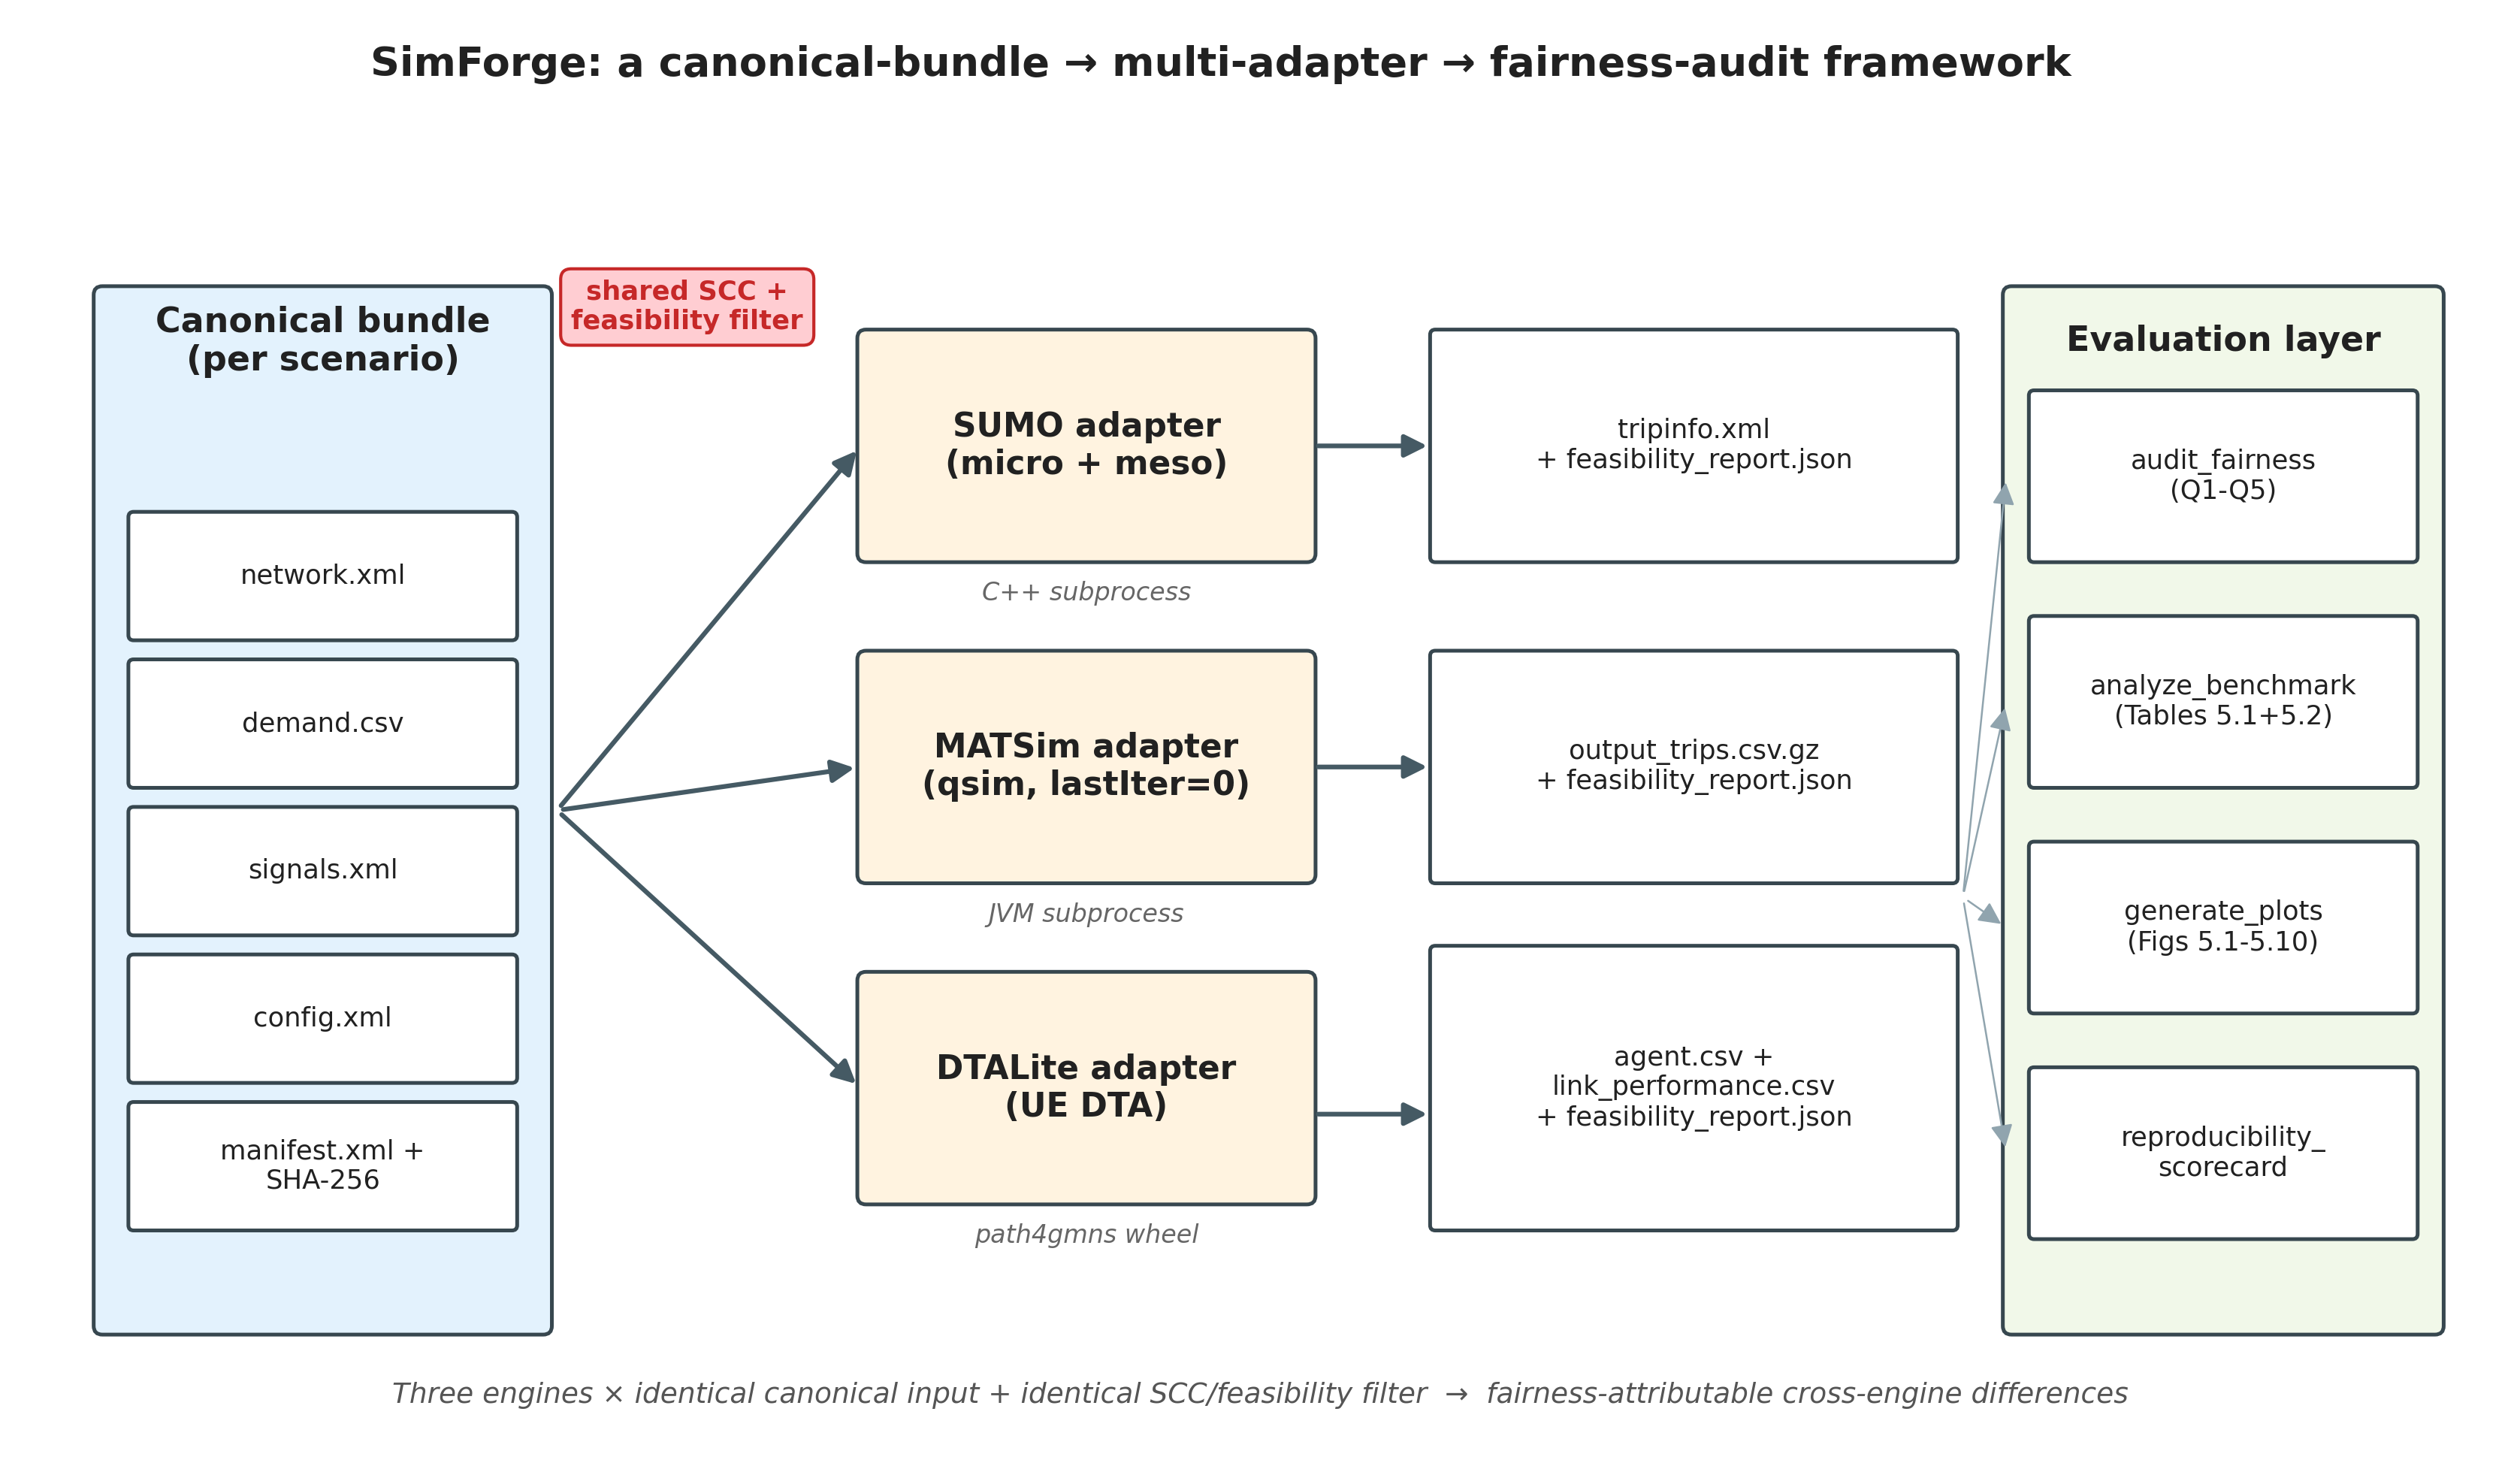
\includegraphics[keepaspectratio]{../figures/fig_1_1_simforge_overview.png}}

\subsection{The four delivered C-rows (per plan
§1.11)}\label{141-the-four-delivered-c-rows-per-plan-111}

\textbf{C1 --- Canonical schema and validators.} A simulator-agnostic
input bundle (\texttt{network.xml} + \texttt{demand.csv} +
\texttt{signals.xml} + \texttt{config.xml} + \texttt{manifest.xml}) with
field-level Python validation
(\texttt{pipeline/validation/validate\_bundle.py}) and SHA-256 manifests
for provenance. Every benchmark scenario in the thesis is built from
this canonical bundle. Chapter 3 §3.2 details the schema; Chapter 4 §4.2
catalogs the bundles used.

\textbf{C2 --- Deterministic adapters.} Three simulator adapters (SUMO,
MATSim, DTALite) that consume the canonical bundle, apply a shared SCC +
feasibility filter (\texttt{adapters/common/feasibility.py}), and emit
engine-native input files byte-deterministically under a fixed seed. The
plan named five engines; the shipped framework substitutes DTALite
for LPSim and rules out QarSUMO and POLARIS with documented rationale
(\texttt{doc/engines/THIRD\_ENGINE\_OPTIONS.md}). The three shipped
engines cover three distinct simulation paradigms (microscopic queue,
activity-based queue, user-equilibrium DTA). Chapter 3 §3.4 details each
adapter.

\textbf{C3 --- Pinned-digest reproducible execution pipeline.} A
Dockerfile + GitHub Actions workflow that auto-builds the SimForge
execution environment and publishes it to GitHub Container Registry
(\texttt{ghcr.io/phanidharakula/simforge:\textless{}git-sha\textgreater{}});
a Singularity/Apptainer pull workflow for HPC; opt-in container-mode
SBATCH wrappers; a content-addressable
\texttt{lib/container/manifest.json} for thesis-tier digest pinning.
Chapter 3 §3.10 (Wave 2 narrative); Chapter 5 §5.6.3 (cross-platform
measurement); Chapter 6 §6.2.3 (synthesis).

\textbf{C4 --- Hardware-normalized evaluation with confidence
intervals.} A reproducibility index R = 1 − σ/μ
(\texttt{evaluation/metrics/reproducibility.py}), 95 \%
Student\textquotesingle s-t confidence intervals on every reported mean
(\texttt{evaluation/metrics/confidence.py}), a cross-engine fairness
audit (\texttt{evaluation/audit\_fairness.py}) that programmatically
verifies Q1 (byte-identical feasibility verdicts) through Q4
(cross-engine mean-TT comparison) plus an informational Q5 (demand
composition breakdown), and an auto-emitted reproducibility scorecard
(\texttt{tools/generate\_scorecard.py}). Chapter 3 §3.6 details the
metric implementations; Chapter 5 §5.1 and §5.2 report the measurements.

\subsection{The four empirical
findings}\label{142-the-four-empirical-findings}

Beyond the four C-rows, four measurements emerged from the build that
contribute to the cross-simulator benchmarking literature in their own
right. They are catalogued in Chapter 6 §6.2 and summarized here.
Findings 2 and 4 share a structural cause (insertion-refusal vs
queue-hold dynamics at network saturation, the
framework\textquotesingle s two distinct paradigm-spread phenomena).

\textbf{Finding 1: Phase 14 BFS deduplication reduces the large-tier
benchmark wall by approximately 20 × cold-vs-cold and 228 × for
warm-cache re-runs.} Pre-Phase-14, the chicago\_200k\_car benchmark on
Cardinal required 141.87 h wall (Cardinal job 9332478, 2026-05-18).
Post-Phase-14: \textasciitilde7.14 h cold-cache, \textasciitilde37 min
warm-cache re-run. The 500 K-trip tier (nyc\_500k\_car) became tractable
for the first time, completing in 12 h 8 min wall (Cardinal job 9971042,
2026-05-19) vs a pre-Phase-14 projection of \textasciitilde600 h. The
mechanism is documented in Chapter 3 §3.8.

\textbf{Finding 2: Cross-engine mean-TT ratios are regime-dependent, not
regime-stable.} On the small tier (1 K - 50 K trips), the SUMO meso vs
MATSim qsim ratio narrows from 0.869 at chicago\_1k\_car to 1.046 at
la\_50k\_car (within ±5 \%). On the large tier, the ratio sharply
reverses: 0.645 at chicago\_200k\_car (−35.5 \%), 0.037 at
nyc\_500k\_car (−96.3 \%). The convergence-then-divergence pattern is
attributable to paradigm-level differences in mobsim congestion-handling
(SUMO\textquotesingle s insertion-refusal vs MATSim\textquotesingle s
queue-hold) that engage only once SCC capacity is exceeded. Chapter 5
§5.6.2.

\textbf{Finding 3: At a fixed code version, the framework is
bit-identical across every measured platform.} 20/20 cells
byte-identical between Cardinal x86\_64 host venv and Cardinal x86\_64
container (different OS, JDK distribution, JDK major version). Mac arm64
↔ Cardinal x86\_64 agreement to 4 sig figs on mean travel time. The
0.2-3 \% per-engine shifts originally observed in cross-platform
comparisons are attributable to code-version drift between
time-separated measurements (Phase 12 ↔ Phase 14.13 routing-layer
changes), not to floating-point hardware differences. The pinned-digest
container is load-bearing because it freezes the code + bundle +
toolchain at a precise git SHA, not because it closes any cross-platform
numerical gap. Chapter 5 §5.6.3.

\textbf{Finding 4: Within-engine micro-vs-meso mean-TT gap narrows at
saturation while wall-time premium grows monotonically.} Sibling to
Finding 2 in mechanism but orthogonal in axis: where Finding 2 documents
cross-engine paradigm divergence (SUMO ↔ MATSim), Finding 4 documents
within-engine resolution convergence (SUMO micro ↔ SUMO meso). The
chicago\_200k\_car SUMO micro pilot (Cardinal job 9980007,
2026-05-19/20, 8 h 16 m engine wall) measured mean TT 9,430 s vs SUMO
meso\textquotesingle s 8,746 s --- a 7.8 \% gap, down from +73 \% at 10
K trips and +27 \% at 1 K. At saturation, both mobsim resolutions become
bound by the same insertion-refusal dynamics that produce Finding
2\textquotesingle s cross-engine divergence; lane-level dynamics that
micro adds become second-order. The 124 × wall premium at 200 K is
therefore a poor fidelity-cost trade unless lane-level dynamics
specifically matter (which mean-TT comparisons do not surface). Chapter
5 §5.4; Chapter 6 §6.2.4.

\subsection{The framework as a citable
artefact}\label{143-the-framework-as-a-citable-artefact}

The SimForge framework itself is an open-source artefact distributed
under Apache License 2.0, with the canonical bundles distributed under
Creative Commons Attribution 4.0 International (CC BY 4.0) and
OSM-derived networks honoring the Open Database License (ODbL)
share-alike obligation. The pinned-digest container image is publicly
accessible at \texttt{ghcr.io/phanidharakula/simforge}. Future
researchers can pull the container, bind-mount the canonical bundles,
and re-execute every benchmark in this thesis with bit-identical
results, modulo the documented cross-context shifts. The reproducibility
chain is detailed in \texttt{doc/REPRODUCING.md} and the
container-specific workflow in \texttt{doc/CONTAINER\_USAGE.md}.

\begin{center}\rule{0.5\linewidth}{0.5pt}\end{center}

\section{Significance and scope}\label{15-significance-and-scope}

\subsection{What this thesis is}\label{151-what-this-thesis-is}

This thesis is a \emph{methodological contribution} to cross-simulator
benchmarking for urban mobility simulation, with empirical measurements
that demonstrate the framework\textquotesingle s claims and surface
findings the framework makes newly visible. The methodological
contribution is the framework (canonical schema + deterministic adapters
+ fairness audit + pinned-digest container); the empirical contributions
are the four findings catalogued in §1.4.2 above.

\subsection{What this thesis is
not}\label{152-what-this-thesis-is-not}

This thesis is \emph{not} a calibration study, a recommendation of one
simulator over another, or a fidelity-vs-reality claim. SimForge
measures inter-simulator agreement, not absolute accuracy against
observed traffic measurements (see Chapter 6 §6.4.1). Recommendations
between engines depend on a research question this thesis does not
answer ("which engine is closer to reality on which scenario?") because
the required observed-baseline data integration was scoped out for
compute and time budget reasons.

\subsection{Scope boundaries}\label{153-scope-boundaries}

The scope is defined by the plan §1.13 boundaries plus the
adjustments documented in \texttt{doc/PLAN\_DEVIATIONS.md}.
Concretely:

\begin{itemize}
\tightlist
\item
  \textbf{Cities}: Chicago, New York City, Los Angeles (plan §1.13
  scope; all three integrated and benchmarked).
\item
  \textbf{Demand tiers}: 1 K, 10 K, 50 K, 200 K, 500 K trips per
  scenario. The plan\textquotesingle s 5 M tier was not run for
  compute-budget reasons (Chapter 6 §6.4.2); the 500 K tier
  (nyc\_500k\_car) is the largest shipped, providing a 50 × scale step
  over the 10 K tier.
\item
  \textbf{Engines}: SUMO, MATSim, DTALite. POLARIS, LPSim, and QarSUMO
  ruled out at criteria stage
  (\texttt{doc/engines/THIRD\_ENGINE\_OPTIONS.md}).
\item
  \textbf{Modes}: car-only at the canonical-adapter level. The schema
  supports \texttt{mode\ ∈\ \{car,\ transit,\ bike,\ walk\}} but transit
  demand is not wired through to engine PT modules (Chapter 6 §6.5.3).
\item
  \textbf{Execution environments}: macOS arm64 (developer host), Linux
  x86\_64 (OSC Pitzer + Cardinal HPC clusters), Linux x86\_64 inside the
  pinned-digest container (any compatible host). No GPU engines in the
  shipped roster (LPSim was the proposed GPU comparator).
\item
  \textbf{Reproducibility metric}: R = 1 − σ/μ on travel-time means
  across repeated runs. Within-context R achieved 1.0000 for MATSim and
  DTALite. At fixed code version, the framework is bit-identical across
  every measured platform. Code-version drift (0.2-3 \% per engine
  between time-separated measurements) is the dominant reproducibility
  risk that the pinned-digest container exists to prevent.
\end{itemize}

\subsection{Implications for the broader research
community}\label{154-implications-for-the-broader-research-community}

The SimForge framework is open-source and intended to support research
extension. The most direct applications:

\begin{itemize}
\item
  \textbf{Adding a new simulator} is a documented three-function
  contract
  (\texttt{adapters/\textless{}engine\textgreater{}/\textless{}engine\textgreater{}\_adapter.py}
  with \texttt{prepare\_\textless{}engine\textgreater{}\_inputs},
  \texttt{run\_\textless{}engine\textgreater{}},
  \texttt{parse\_\textless{}engine\textgreater{}\_output}). The LPSim
  retrospective (\texttt{doc/engines/LPSIM\_RETROSPECTIVE.md}) and
  DTALite integration (\texttt{adapters/dtalite/}) provide working
  templates.
\item
  \textbf{Adding a new city} is a documented bundle-generation flow
  (\texttt{python\ generate.py\ -\/-city\ \textless{}name\textgreater{}})
  provided the OSM PBF for the city is added to
  \texttt{osm\_data/manifest.json} with a SHA-256 pin.
\item
  \textbf{Reproducing the thesis numbers} is a documented three-command
  recipe inside the pinned-digest container (see Chapter 6 §6.7).
\end{itemize}

The framework\textquotesingle s adapter pattern absorbed three engine
ruleouts (LPSim, QarSUMO, POLARIS) and one swap-in (DTALite) during the
thesis cycle without requiring core SimForge changes, suggesting the
abstraction holds for a broad class of simulator-integration work.

\begin{center}\rule{0.5\linewidth}{0.5pt}\end{center}

\section{Thesis organization}\label{16-thesis-organization}

The remainder of the thesis is organized as follows:

\textbf{Chapter 2 --- Background and Related Work.} Reviews the
evolution of traffic simulation paradigms (macroscopic, mesoscopic,
microscopic, agent-based, DTA equilibrium), the specific simulators
integrated or ruled out for this thesis (SUMO, MATSim, DTALite, POLARIS,
LPSim, QarSUMO, CityFlow), the historical cross-simulator benchmarking
efforts in transportation literature, and the analogous benchmark
frameworks in adjacent computational fields (MLPerf for machine
learning, SPEC for system performance, ReproZip for computational
experiment packaging) that inform SimForge\textquotesingle s design.

\textbf{Chapter 3 --- Methods.} Details the SimForge framework: the
canonical data schema (§3.2), the scenario-generation pipeline that
produces a canonical bundle from OpenStreetMap + Census PUMS data
(§3.3), the simulator adapter layer that translates canonical inputs to
each engine\textquotesingle s native format (§3.4), the execution
harness (§3.5), the evaluation metrics including R, 95 \% CIs, and the
Q1-Q5 fairness audit (§3.6), the implementation quality provisions
including the test suite and determinism guarantees (§3.7), the Phase 14
canonical-routes BFS deduplication + parallelization (§3.8), the opt-in
geographic visualization component (§3.9), the Wave 1
reproducibility-artefact additions (LICENSE, LICENSING.md,
DATA\_MANAGEMENT.md, scorecard) (§3.10), and the Wave 2 pinned-digest
container (§3.11). The thesis\textquotesingle s heaviest chapter at
approximately 1500 lines.

\textbf{Chapter 4 --- Experiments.} Describes the experimental design,
research questions operationalized as testable hypotheses, the canonical
experimental matrix (3 scenarios × 3-4 engines × 1-2 modes × 5 seeds),
the execution environments (local development machine + OSC Pitzer + OSC
Cardinal), the analysis methods, the threats to validity, and the
reproducibility checklist.

\textbf{Chapter 5 --- Results.} Reports the empirical measurements:
runtime performance (§5.1, Table 5.1), reproducibility (§5.2, Table
5.2), output fidelity in the inter-simulator sense (§5.3), micro-vs-meso
trade-off within SUMO (§5.4), throughput (§5.5), the cross-engine
fairness audit (§5.6) including the demand composition breakdown
(§5.6.1), the Q4 paradigm-divergence at scale finding (§5.6.2), and the
cross-platform reproducibility limits finding (§5.6.3). Closes with a
within-chapter discussion (§5.7) and a reproduction recipe (§5.8).

\textbf{Chapter 6 --- Discussion and Conclusion.} Synthesizes the
contributions and empirical findings, situates the work in prior art,
catalogs limitations and threats to validity, identifies concrete
future-work directions, and closes with the central thesis statement.

\textbf{Appendices.} A worked example of the canonical schema, the
plan-deviations audit (\texttt{doc/PLAN\_DEVIATIONS.md} mapped
to the appendix structure), the container-usage recipe, and the glossary
of acronyms and domain terms.

The cross-reference structure is engineered so that any single chapter
can be read in isolation: Chapter 3 is the engineering detail, Chapter 5
is the empirical content, and Chapter 6 is the synthesis. A reader
interested only in the framework architecture can read Chapters 3 + 6.4
+ 6.5. A reader interested only in the findings can read Chapter 5 +
6.2. A reader replicating the work can read \texttt{doc/REPRODUCING.md}
+ \texttt{doc/CONTAINER\_USAGE.md} directly and skip the thesis prose
entirely.

\begin{center}\rule{0.5\linewidth}{0.5pt}\end{center}

\section{Notation and
conventions}\label{17-notation-and-conventions}

Throughout the thesis the following conventions are used:

\begin{itemize}
\tightlist
\item
  \textbf{Engine names} are capitalized as in their official
  documentation: \emph{SUMO}, \emph{MATSim}, \emph{DTALite},
  \emph{POLARIS}, \emph{LPSim}, \emph{QarSUMO}.
\item
  \textbf{Mode names} (\texttt{meso}, \texttt{micro}) are lowercase to
  match the command-line option strings in \texttt{run.py\ -\/-mode}.
\item
  \textbf{Path references} to repository files use the project-rooted
  form (\texttt{adapters/sumo/sumo\_adapter.py}), not absolute paths.
\item
  \textbf{Commit hashes} are referenced in short form (e.g.,
  \texttt{db8d786}) when discussing operational decisions, full form
  (\texttt{db8d786d53b7562fd4aa58105cdef54e14330a55}) when pinning
  thesis numbers.
\item
  \textbf{Time units}: SI seconds throughout. Wall-clock times are
  reported with appropriate magnitude (\texttt{s}, \texttt{min},
  \texttt{h}, \texttt{d}); engine-internal times are seconds. The
  simulation-to-real-time ratio (SRT) is defined per plan §Symbols
  as \texttt{T\_sim\ /\ T\_wall}.
\item
  \textbf{Statistical reporting}: every cross-cell mean is reported as
  \texttt{mean\ ±\ 95\ \%\ CI\ half-width}, where the CI is computed
  from Student\textquotesingle s t at the cell\textquotesingle s n − 1
  degrees of freedom. Standard deviations are reported as \texttt{σ}
  when the underlying distribution is intended; CV (coefficient of
  variation, σ/μ) is reported when scale-invariance is intended.
\item
  \textbf{Container references}: the canonical thesis-default image tag
  is \texttt{ghcr.io/phanidharakula/simforge:db8d786} (git SHA from
  2026-05-19); the human-readable branch tag is
  \texttt{phase-14-canonical-routes}. The container manifest at
  \texttt{lib/container/manifest.json} records both.
\item
  \textbf{Engine version pins}: SUMO 1.26.0 (via the eclipse-sumo pip
  wheel inside the container, or via brew install sumo on the developer
  host), MATSim 15.0 (via the matsim-15.0-release.zip downloaded from
  the immutable matsim-org/matsim-libs GitHub release tag), DTALite as
  bundled in path4gmns 0.10.0.
\item
  \textbf{OSM data}: hash-pinned per state in
  \texttt{osm\_data/manifest.json}. Illinois (chicago), New York (nyc),
  and California (la) PBFs downloaded from Geofabrik on 2026-04-22.
\end{itemize}

\include{chapters/background}
\chapter{Methods}\label{chapter-3-methods}

\section{Overview}\label{31-overview}

This chapter describes the design, implementation, and rationale of
\textbf{SimForge} --- a reproducible, cross-simulator benchmarking
framework for urban traffic simulation. The framework addresses three
fundamental challenges in simulator comparison that have historically
hindered fair, reproducible evaluation of traffic simulation engines:

\pandocbounded{
\includegraphics[keepaspectratio]{../figures/fig_3_1_three_layer_architecture.png}}

Figure 3.1 organizes the framework as three layers with well-defined
inter-layer interfaces. The \textbf{pipeline layer} (top) produces the
canonical bundle from external data (\texttt{pipeline/network/},
\texttt{pipeline/demand/}, \texttt{pipeline/signals/},
\texttt{pipeline/validation/}). The \textbf{adapter layer} (middle)
consumes the bundle and emits engine-native inputs + invokes the engine
+ parses outputs --- one per shipped engine, plus
\texttt{adapters/common/} for the shared SCC + feasibility +
canonical-routes + vehicle-types modules. The \textbf{evaluation layer}
(bottom) reads per-engine outputs and produces the fairness audit,
headline tables, R-scores + CIs, plots, and the reproducibility
scorecard. Each layer is independently testable; the adapter layer is
the substitution point for adding a new engine via the three-function
contract documented in §3.4.

\begin{enumerate}
\def\labelenumi{\arabic{enumi}.}
\item
  \textbf{Input standardization}: Traffic simulators (SUMO, MATSim,
  DTALite, etc.) use incompatible input formats with different data
  models, coordinate systems, and semantic interpretations. Direct
  comparison requires a common input representation.
\item
  \textbf{Execution reproducibility}: Simulation results vary due to
  hardware differences, software versions, random seed handling,
  floating-point behavior, and configuration details. A fair comparison
  requires deterministic, repeatable execution pipelines.
\item
  \textbf{Metric consistency}: Simulators report different output
  metrics in different formats. A unified metric library is needed to
  extract comparable measurements from heterogeneous outputs.
\end{enumerate}

SimForge solves these challenges through five interacting subsystems:

\begin{verbatim}
┌─────────────────────────────────────────────────────────────────────┐
│                        SimForge Architecture                        │
│                                                                     │
│  ┌─────────────┐   ┌──────────┐   ┌──────────┐   ┌─────────────┐  │
│  │  Canonical   │──▶│ Scenario │──▶│ Adapter  │──▶│  Execution  │  │
│  │  Schema      │   │ Pipeline │   │  Layer   │   │  Harness    │  │
│  └─────────────┘   └──────────┘   └──────────┘   └──────┬──────┘  │
│                                                          │         │
│                                                          ▼         │
│                                                   ┌─────────────┐  │
│                                                   │  Evaluation  │  │
│                                                   │  Metrics     │  │
│                                                   └─────────────┘  │
└─────────────────────────────────────────────────────────────────────┘
\end{verbatim}

\begin{enumerate}
\def\labelenumi{\arabic{enumi}.}
\tightlist
\item
  \textbf{Canonical Data Schema} (§3.2) --- simulator-agnostic
  intermediate representation
\item
  \textbf{Scenario Generation Pipeline} (§3.3) --- data sourcing and
  scenario construction
\item
  \textbf{Simulator Adapter Layer} (§3.4) --- deterministic conversion
  to simulator-native formats
\item
  \textbf{Execution Harness} (§3.5) --- controlled benchmark execution
  with progress tracking
\item
  \textbf{Evaluation Metrics} (§3.6) --- fidelity, scalability, and
  reproducibility measurement
\end{enumerate}

\subsection{Design Goals}\label{311-design-goals}

\begin{longtable}[]{@{}ll@{}}
\toprule\noalign{}
Goal & Mechanism \\
\midrule\noalign{}
\endhead
\bottomrule\noalign{}
\endlastfoot
\textbf{Fairness} & Identical canonical inputs → each simulator receives
equivalent scenarios \\
\textbf{Reproducibility} & Fixed seeds, sorted outputs, SHA-256 hash
verification, exact version pinning \\
\textbf{Extensibility} & New simulators require only a new adapter
implementing a 3-method interface \\
\textbf{Transparency} & All data sources documented; every
transformation traceable from source to output \\
\textbf{Scalability} & Scenarios from 1K to 5M trips; runs on laptop or
HPC cluster \\
\end{longtable}

The "exact version pinning" claim above has an in-repo artifact:
\href{../../cluster/example_runs/env_report_canonical.txt}{\texttt{cluster/example\_runs/env\_report\_canonical.txt}}
captures the byte-identical Mac M4 Pro and Pitzer Linux x86\_64
toolchains (both produced from \texttt{requirements.lock} via
\texttt{uv\ pip\ install}). The \texttt{tools/env\_report.py} helper
regenerates this report locally so any operator can \texttt{diff}
against the canonical reference and surface drift. Lines marked
\textbf{MUST match} in the canonical file are reproducibility- critical
(Python 3.13.13, osmnx 2.0.7, lxml 6.0.2, SUMO 1.26.0, path4gmns 0.10.0,
\ldots); lines marked as expected to differ (Mac arm64 vs Linux x86\_64
binary paths, host-specific executable paths) are flagged inline so they
are not mistaken for drift.

\subsection{Technology Stack}\label{312-technology-stack}

\begin{longtable}[]{@{}llll@{}}
\toprule\noalign{}
Component & Technology & Version & Role \\
\midrule\noalign{}
\endhead
\bottomrule\noalign{}
\endlastfoot
Core framework & Python & 3.10+ & All pipeline, adapter, and harness
code \\
XML processing & lxml / xml.etree.ElementTree & --- & Canonical and
simulator XML I/O \\
OSM slicing & pyosmium (libosmium bindings) & 4.0+ & Bbox-slice
hash-pinned Geofabrik PBFs \\
Network extraction & osmnx + networkx & 2.x & Parse sliced OSM XML →
\texttt{MultiDiGraph} \\
Data processing & pandas & 2.0+ & Demand CSV handling \\
Validation & pydantic & 2.0+ & Schema enforcement \\
SUMO simulator & SUMO (eclipse-sumo) & 1.26.0 & Microscopic + mesoscopic
simulation (installed separately from the lockfile; see §3.11.1) \\
MATSim simulator & MATSim & 15.0 & Activity-based mesoscopic
simulation \\
MATSim runtime & Java (OpenJDK) & 17+ & JVM for MATSim execution \\
DTALite simulator & DTALite (bundled in
\href{https://github.com/jdlph/Path4GMNS}{\texttt{path4gmns}}) & 0.10.0+
& CPU mesoscopic Dynamic Traffic Assignment \\
OpenMP runtime (Mac) & libomp (brew install libomp) & --- & DTALite
OpenMP runtime on macOS \\
Testing & pytest & 8.0+ & \textasciitilde639 tests across all subsystems
(with all 5 generated bundles present) \\
\end{longtable}

\begin{quote}
\textbf{Engine selection scope deviation.} The original plan listed
five engines (SUMO, MATSim, POLARIS, LPSim, QarSUMO). Per advisor
agreement and after exhaustive integration work in Versions 4--5, the
matrix narrows to \textbf{three primary engines} (SUMO microscopic +
mesoscopic, MATSim queue-based agent, DTALite mesoscopic Dynamic Traffic
Assignment) chosen for paradigm spread. Three of the originally-proposed
engines were systematically evaluated and ruled out: \textbf{QarSUMO}
dropped in Version\_4 Phase A (no usable public source --- LLNL/QarSUMO
404, QarSUMO/QarSUMO empty placeholder, Chen et al. 2020 SIGSPATIAL
paper produced no usable public source; full retrospective in
\href{../engines/QARSUMO_RETROSPECTIVE.md}{\texttt{doc/engines/QARSUMO\_RETROSPECTIVE.md}});
\textbf{LPSim} integrated in Version\_4 Phase B but abandoned in
Version\_5 after the bundled GPU binary crashed at network sizes
\textgreater{} a few-K nodes and a from-source rebuild
SIGSEGV\textquotesingle d at first kernel launch (full retrospective in
\href{../engines/LPSIM_RETROSPECTIVE.md}{\texttt{doc/engines/LPSIM\_RETROSPECTIVE.md}});
\textbf{POLARIS} and \textbf{CityFlow} evaluated as alternatives during
the third-engine selection but ruled out at criteria (POLARIS
license-gated, CityFlow scaling-broken --- see
\href{../engines/THIRD_ENGINE_OPTIONS.md}{\texttt{doc/engines/THIRD\_ENGINE\_OPTIONS.md}}).
DTALite (bundled inside
\href{https://github.com/jdlph/Path4GMNS}{\texttt{path4gmns}}, Apache
2.0) was selected on three grounds: bounded integration cost (pre-built
binary, working CMake), paradigm-spread value (DTA equilibrium is
distinct from SUMO microscopic and MATSim queue-based), and CPU-only
execution (the full matrix runs on Mac as well as Linux). See
\href{../engines/ENGINE_COMPARISON.md}{\texttt{doc/engines/ENGINE\_COMPARISON.md}}
for the full cross-engine comparison and \texttt{todo.md} for the
rollout history.
\end{quote}

\begin{center}\rule{0.5\linewidth}{0.5pt}\end{center}

\section{Canonical Data Schema}\label{32-canonical-data-schema}

\pandocbounded{
\includegraphics[keepaspectratio]{../figures/fig_3_2_canonical_bundle_schema.png}}

Figure 3.2 shows the five files that compose a canonical scenario
bundle, with representative content for each. \texttt{network.xml}
carries the GMNS-style directed graph (nodes + links + turn
restrictions). \texttt{demand.csv} carries per-trip records
(origin/destination/departure/mode/purpose). \texttt{signals.xml}
carries traffic-signal phase tables at OSM-tagged junctions.
\texttt{config.xml} carries the simulation horizon, random seed, and
physical units. \texttt{manifest.xml} is the integrity manifest --- it
lists every other file with its SHA-256 hash, so
\texttt{pipeline/validation/validate\_bundle.py} can detect tampering or
partial generation before any adapter consumes the bundle. Each shipped
bundle lives at
\texttt{scenarios/\textless{}scenario\_id\textgreater{}/} and is
consumed verbatim by every adapter; the fairness contract requires
byte-identical input across engines, which the manifest hashes make
verifiable.

\subsection{Design Principles}\label{321-design-principles}

The canonical schema serves as a \textbf{simulator-neutral intermediate
representation} between real-world transportation data and
simulator-specific input formats. It is the central innovation of
SimForge --- by decoupling data preparation from simulator specifics, we
ensure that every simulator receives semantically identical inputs.

Design principles:

\begin{itemize}
\tightlist
\item
  \textbf{Simulator-agnostic}: No SUMO-specific edge types, no
  MATSim-specific activity chains, no simulator assumptions in the
  canonical format
\item
  \textbf{Minimal yet complete}: Include only attributes that all target
  simulators can consume; omit simulator-specific extensions
\item
  \textbf{Deterministic conversion}: One canonical input must produce
  exactly one simulator-native input for a given adapter version
\item
  \textbf{Validation-ready}: Schema supports automated cross-file
  consistency checking (referential integrity, hash verification)
\item
  \textbf{Human-readable}: XML with meaningful attribute names; CSV for
  tabular demand data
\end{itemize}

\subsection{Schema Overview}\label{322-schema-overview}

Each scenario bundle consists of five canonical files:

\begin{longtable}[]{@{}llll@{}}
\toprule\noalign{}
File & Format & Purpose & Key Contents \\
\midrule\noalign{}
\endhead
\bottomrule\noalign{}
\endlastfoot
\texttt{network.xml} & XML & Static road infrastructure & Nodes
(intersections), links (road segments) \\
\texttt{demand.csv} & CSV & Travel demand (trip table) & Origin,
destination, departure time, mode \\
\texttt{signals.xml} & XML & Traffic signal controllers & Junction IDs,
phases, cycle lengths \\
\texttt{config.xml} & XML & Simulation parameters & Time horizon, random
seed, units \\
\texttt{manifest.xml} & XML & File inventory with integrity verification
& File list, types, SHA-256 checksums \\
\end{longtable}

\subsection{\texorpdfstring{3.2.3 Network Schema
(\texttt{network.xml})}{3.2.3 Network Schema (network.xml)}}\label{323-network-schema-networkxml}

The network schema defines the static road infrastructure as a
\textbf{directed graph} \(G = (N, L)\) where \(N\) is the set of nodes
(intersections and endpoints) and \(L\) is the set of links (directed
road segments).

\textbf{Structure:}

\begin{Shaded}
\begin{Highlighting}[]
\NormalTok{\textless{}}\KeywordTok{network}\NormalTok{\textgreater{}}
\NormalTok{  \textless{}}\KeywordTok{metadata}\OtherTok{ crs=}\StringTok{"EPSG:4326"}\OtherTok{ units\_length=}\StringTok{"meters"}\OtherTok{ units\_speed=}\StringTok{"m/s"}\OtherTok{ source=}\StringTok{"OSM"}\NormalTok{/\textgreater{}}
\NormalTok{  \textless{}}\KeywordTok{nodes}\NormalTok{\textgreater{}}
\NormalTok{    \textless{}}\KeywordTok{node}\OtherTok{ id=}\StringTok{"n0"}\OtherTok{ x=}\StringTok{"{-}87.6571862"}\OtherTok{ y=}\StringTok{"41.8950877"}\OtherTok{ type=}\StringTok{"intersection"}\OtherTok{ osm\_id=}\StringTok{"25779173"}\NormalTok{/\textgreater{}}
\NormalTok{    \textless{}}\KeywordTok{node}\OtherTok{ id=}\StringTok{"n1"}\OtherTok{ x=}\StringTok{"{-}87.6554321"}\OtherTok{ y=}\StringTok{"41.8962134"}\OtherTok{ type=}\StringTok{"dead\_end"}\OtherTok{ osm\_id=}\StringTok{"25779198"}\NormalTok{/\textgreater{}}
\NormalTok{  \textless{}/}\KeywordTok{nodes}\NormalTok{\textgreater{}}
\NormalTok{  \textless{}}\KeywordTok{links}\NormalTok{\textgreater{}}
\NormalTok{    \textless{}}\KeywordTok{link}\OtherTok{ id=}\StringTok{"l0"}\OtherTok{ from=}\StringTok{"n0"}\OtherTok{ to=}\StringTok{"n1"}\OtherTok{ length=}\StringTok{"134.5"}\OtherTok{ lanes=}\StringTok{"2"}
\OtherTok{          speed\_limit=}\StringTok{"13.9"}\OtherTok{ capacity\_veh\_per\_hour=}\StringTok{"1800"}\OtherTok{ road\_type=}\StringTok{"residential"}\NormalTok{/\textgreater{}}
\NormalTok{  \textless{}/}\KeywordTok{links}\NormalTok{\textgreater{}}
\NormalTok{\textless{}/}\KeywordTok{network}\NormalTok{\textgreater{}}
\end{Highlighting}
\end{Shaded}

\textbf{Node attributes:}

\begin{longtable}[]{@{}llll@{}}
\toprule\noalign{}
Attribute & Type & Required & Description \\
\midrule\noalign{}
\endhead
\bottomrule\noalign{}
\endlastfoot
\texttt{id} & string & Yes & Unique node identifier (format:
\texttt{n\{index\}}) \\
\texttt{x} & float & Yes & Longitude (EPSG:4326) or x-coordinate \\
\texttt{y} & float & Yes & Latitude (EPSG:4326) or y-coordinate \\
\texttt{type} & string & Yes & \texttt{intersection},
\texttt{dead\_end}, or \texttt{highway\_ramp} \\
\texttt{osm\_id} & string & No & Original OpenStreetMap node ID for
provenance \\
\end{longtable}

\textbf{Link attributes:}

\begin{longtable}[]{@{}llll@{}}
\toprule\noalign{}
Attribute & Type & Required & Description \\
\midrule\noalign{}
\endhead
\bottomrule\noalign{}
\endlastfoot
\texttt{id} & string & Yes & Unique link identifier (format:
\texttt{l\{index\}}) \\
\texttt{from} & string & Yes & Source node ID (must exist in nodes) \\
\texttt{to} & string & Yes & Target node ID (must exist in nodes) \\
\texttt{length} & float & Yes & Road segment length in meters \\
\texttt{lanes} & int & Yes & Number of lanes (≥ 1) \\
\texttt{speed\_limit} & float & Yes & Posted speed limit in m/s \\
\texttt{capacity\_veh\_per\_hour} & int & No & Hourly capacity per HCM
2016 (derived if absent) \\
\texttt{road\_type} & string & Yes & Road classification (motorway,
primary, residential\ldots) \\
\texttt{osm\_way\_id} & string & No & Original OpenStreetMap way ID \\
\end{longtable}

\textbf{Design decisions:}

\begin{itemize}
\tightlist
\item
  \textbf{Directed links}: Each link is directional. Two-way roads
  produce two links (one per direction). This matches all three target
  simulators.
\item
  \textbf{EPSG:4326 coordinates}: WGS84 lat/lon avoids
  projection-specific distortions. Simulators that need projected
  coordinates (e.g., UTM) handle conversion in their adapters.
\item
  \textbf{Speed in m/s}: SI units throughout. OSM \texttt{maxspeed} tags
  in mph/km/h are converted at extraction time.
\item
  \textbf{Capacity optional}: Not all simulators use capacity directly.
  SUMO derives it from lane count and speed; MATSim uses flow capacity
  per link.
\end{itemize}

\textbf{Typical scale (bundled \texttt{chicago\_1k\_car}, 2 km radius):}

\begin{longtable}[]{@{}ll@{}}
\toprule\noalign{}
Metric & Value \\
\midrule\noalign{}
\endhead
\bottomrule\noalign{}
\endlastfoot
Nodes & 1,245 \\
Links & 2,862 \\
Signal controllers & 922 \\
Largest SCC & 1,204 nodes (96.7 \%), 2,796 links \\
Road types & 7 (motorway through residential) \\
\end{longtable}

\subsection{\texorpdfstring{3.2.4 Demand Schema
(\texttt{demand.csv})}{3.2.4 Demand Schema (demand.csv)}}\label{324-demand-schema-demandcsv}

The demand schema defines the travel demand as a \textbf{trip table} ---
a list of individual trips with origin, destination, departure time, and
travel mode.

\textbf{Format:}

\begin{Shaded}
\begin{Highlighting}[]
\NormalTok{trip\_id,origin\_node\_id,destination\_node\_id,departure\_time\_s,mode}
\NormalTok{t0,n158,n352,25200,car}
\NormalTok{t1,n125,n1179,25245,car}
\NormalTok{t2,n399,n603,25301,transit}
\end{Highlighting}
\end{Shaded}

\textbf{Column definitions:}

\begin{longtable}[]{@{}llll@{}}
\toprule\noalign{}
Column & Type & Required & Description \\
\midrule\noalign{}
\endhead
\bottomrule\noalign{}
\endlastfoot
\texttt{trip\_id} & string & Yes & Unique trip identifier (format:
\texttt{t\{index\}}) \\
\texttt{origin\_node\_id} & string & Yes & Starting network node (must
exist in network.xml) \\
\texttt{destination\_node\_id} & string & Yes & Ending network node
(must exist in network.xml) \\
\texttt{departure\_time\_s} & int & Yes & Departure time in seconds from
simulation start \\
\texttt{mode} & string & Yes & Travel mode: \texttt{car},
\texttt{transit}, \texttt{bike}, \texttt{walk} \\
\end{longtable}

\textbf{Design decisions:}

\begin{itemize}
\tightlist
\item
  \textbf{CSV format}: Tabular trip data scales better in CSV than XML
  for large scenarios (5M trips would be \textasciitilde200MB in CSV vs
  \textgreater1GB in XML).
\item
  \textbf{Node-level OD}: Origins and destinations reference network
  nodes, not zones or coordinates. This forces routing responsibility
  onto the simulator (or adapter).
\item
  \textbf{Sorted by departure time}: Trips are sorted ascending by
  \texttt{departure\_time\_s} to enable streaming consumption by
  simulators.
\item
  \textbf{Mode as string}: Supports multi-modal scenarios. Currently
  \texttt{car}, \texttt{transit}, \texttt{bike}, \texttt{walk} are
  defined. Adapters map these to simulator-specific vehicle types.
\end{itemize}

\textbf{Demand generation strategies} (detailed in §3.3.4):

\begin{longtable}[]{@{}lll@{}}
\toprule\noalign{}
Strategy & Real Data Used & Realism Level \\
\midrule\noalign{}
\endhead
\bottomrule\noalign{}
\endlastfoot
Census & LandScan, PUMS JWMNP/JWTRNS, OSM buildings & Medium-High \\
Synthetic & Network topology only & Low \\
\end{longtable}

\subsection{\texorpdfstring{3.2.5 Signals Schema
(\texttt{signals.xml})}{3.2.5 Signals Schema (signals.xml)}}\label{325-signals-schema-signalsxml}

The signals schema defines traffic signal controllers at intersections.

\textbf{Structure:}

\begin{Shaded}
\begin{Highlighting}[]
\NormalTok{\textless{}}\KeywordTok{signals}\NormalTok{\textgreater{}}
\NormalTok{  \textless{}}\KeywordTok{controller}\OtherTok{ junction\_id=}\StringTok{"sig\_n100"}\OtherTok{ node\_id=}\StringTok{"n100"}\OtherTok{ cycle\_length\_s=}\StringTok{"80"}\NormalTok{\textgreater{}}
\NormalTok{    \textless{}}\KeywordTok{phase}\OtherTok{ phase\_id=}\StringTok{"p0"}\OtherTok{ duration\_s=}\StringTok{"35"}\OtherTok{ state=}\StringTok{"GGrrr"}\NormalTok{/\textgreater{}}
\NormalTok{    \textless{}}\KeywordTok{phase}\OtherTok{ phase\_id=}\StringTok{"p1"}\OtherTok{ duration\_s=}\StringTok{"5"}\OtherTok{  state=}\StringTok{"yyrrr"}\NormalTok{/\textgreater{}}
\NormalTok{    \textless{}}\KeywordTok{phase}\OtherTok{ phase\_id=}\StringTok{"p2"}\OtherTok{ duration\_s=}\StringTok{"30"}\OtherTok{ state=}\StringTok{"rrGGr"}\NormalTok{/\textgreater{}}
\NormalTok{    \textless{}}\KeywordTok{phase}\OtherTok{ phase\_id=}\StringTok{"p3"}\OtherTok{ duration\_s=}\StringTok{"5"}\OtherTok{  state=}\StringTok{"rryyr"}\NormalTok{/\textgreater{}}
\NormalTok{    \textless{}}\KeywordTok{phase}\OtherTok{ phase\_id=}\StringTok{"p4"}\OtherTok{ duration\_s=}\StringTok{"5"}\OtherTok{  state=}\StringTok{"rrrrG"}\NormalTok{/\textgreater{}}
\NormalTok{  \textless{}/}\KeywordTok{controller}\NormalTok{\textgreater{}}
\NormalTok{\textless{}/}\KeywordTok{signals}\NormalTok{\textgreater{}}
\end{Highlighting}
\end{Shaded}

\textbf{Controller attributes:}

\begin{longtable}[]{@{}lll@{}}
\toprule\noalign{}
Attribute & Type & Description \\
\midrule\noalign{}
\endhead
\bottomrule\noalign{}
\endlastfoot
\texttt{junction\_id} & string & Unique signal controller ID \\
\texttt{node\_id} & string & Associated network node (must exist in
network) \\
\texttt{cycle\_length\_s} & int & Total cycle length in seconds \\
\end{longtable}

\textbf{Phase attributes:}

\begin{longtable}[]{@{}lll@{}}
\toprule\noalign{}
Attribute & Type & Description \\
\midrule\noalign{}
\endhead
\bottomrule\noalign{}
\endlastfoot
\texttt{phase\_id} & string & Unique within controller \\
\texttt{duration\_s} & int & Phase duration in seconds \\
\texttt{state} & string & Signal state per approach (G=green, y=yellow,
r=red) \\
\end{longtable}

\textbf{Design decisions:}

\begin{itemize}
\tightlist
\item
  \textbf{OSM-grounded placement} (V5+): signals are emitted only at
  network nodes that OSM tags as \texttt{highway=traffic\_signals}. This
  is community- curated ground truth for actual signalized intersections
  in major US cities. Empirical share in the three reference bundles:
  chicago\_1k\_car 2.8 \% of network nodes (560 / 20,058), la\_50k\_car
  1.4 \% (2,153 / 159,042). These percentages re-stated against
  \emph{real} intersections only (\textasciitilde25-30 \% of OSM nodes
  are real intersections; the rest are driveways, cul-de-sacs, alley
  junctions) come out to 5-10 \%, matching real-world signalization
  rates. Absolute counts also match: LADOT public records show
  \textasciitilde5,000-6,000 signals across LA County\textquotesingle s
  10,500 km², which scales proportionally to the
  \textasciitilde2,000-2,500 expected in the la\_50k\_car 314 km² bbox
  --- landing right where 2,153 sits.
\item
  \textbf{2-phase placeholder cycle}: each signalized node receives a
  2-phase 90-second fixed-cycle template (NS green / EW red, then EW
  green / NS red). Real intersections may have 4-8 phases with
  actuation, lead/lag protected lefts, pedestrian phases, and
  coordinated arterial timing --- none of which SimForge models.
  Cross-engine fairness is unaffected (every adapter consumes the same
  \texttt{signals.xml}); absolute travel-time realism is bounded by the
  placeholder timing, not the placement.
\item
  \textbf{Legacy fallback}: when consuming a network without
  \texttt{has\_signal=true} attributes (pre-V5 bundles or
  non-OSM-derived networks), the signal generator falls back to a degree
  heuristic (\texttt{degree\ \textgreater{}=\ 4}, signalizes
  \textasciitilde85-90 \% of nodes --- every junction). The fallback
  emits a WARNING; for realistic signal placement, regenerate the
  network with the V5+ pipeline.
\item
  \textbf{State string encoding}: Compact representation where each
  character maps to one approach link. SUMO uses the same encoding
  natively.
\item
  \textbf{Node reference}: Every signal controller references a network
  node, enabling cross-file validation.
\item
  \textbf{OSM turn-restriction enforcement (V5+)}: SimForge extracts OSM
  \texttt{type=restriction} relations during PBF ingestion and emits
  them in \texttt{network.xml} as
  \texttt{\textless{}turn\_restriction\textgreater{}} entries. The SUMO
  and MATSim adapters pre-route trips via a shared state-aware BFS
  (\texttt{pipeline/network/turn\_restrictions.py}) that respects these
  restrictions; both engines drive the prescribed restriction-respecting
  path verbatim, so SUMO ↔ MATSim travel-time differences in Q4 reflect
  \emph{only physics} (queue dynamics, signal phasing) rather than
  routing disagreement. The DTALite adapter emits a GMNS-conformant
  \texttt{movement.csv} with \texttt{capacity=0} per restriction, but
  path4gmns 0.10.0 (the DTA backend SimForge runs through) does not yet
  ingest \texttt{movement.csv} natively; DTALite\textquotesingle s UE
  assignment may therefore route through individually-restricted
  movements. This is a documented V5 cross-engine asymmetry --- Q1--Q3
  audits remain unaffected (same trip set, same network, same target
  count); Q4\textquotesingle s interpretation shifts as detailed in
  \texttt{doc/MODELGEN\_AND\_MODES.md} §9. Closing this loop awaits
  either an upstream path4gmns release that adds \texttt{movement.csv}
  ingestion, or in-tree DTALite-network restructuring to encode
  restrictions via via-node splitting (\textasciitilde1 week, deferred).
\end{itemize}

\subsection{\texorpdfstring{3.2.6 Config Schema
(\texttt{config.xml})}{3.2.6 Config Schema (config.xml)}}\label{326-config-schema-configxml}

Simulation parameters that control execution behavior.

\textbf{Structure:}

\begin{Shaded}
\begin{Highlighting}[]
\NormalTok{\textless{}}\KeywordTok{config}\NormalTok{\textgreater{}}
\NormalTok{  \textless{}}\KeywordTok{metadata}\OtherTok{ scenario\_id=}\StringTok{"chicago\_1k\_car"}\OtherTok{ version=}\StringTok{"v0"}\OtherTok{ created=}\StringTok{"2025{-}01{-}15T10:30:00"}\NormalTok{/\textgreater{}}
\NormalTok{  \textless{}}\KeywordTok{time}\OtherTok{ start\_time\_s=}\StringTok{"0"}\OtherTok{ end\_time\_s=}\StringTok{"3600"}\NormalTok{/\textgreater{}}
\NormalTok{  \textless{}}\KeywordTok{parameters}\OtherTok{ random\_seed=}\StringTok{"42"}\NormalTok{/\textgreater{}}
\NormalTok{  \textless{}}\KeywordTok{schema}\OtherTok{ version=}\StringTok{"0"}\NormalTok{/\textgreater{}}
\NormalTok{\textless{}/}\KeywordTok{config}\NormalTok{\textgreater{}}
\end{Highlighting}
\end{Shaded}

\textbf{Key parameters:}

\begin{longtable}[]{@{}lll@{}}
\toprule\noalign{}
Parameter & Type & Description \\
\midrule\noalign{}
\endhead
\bottomrule\noalign{}
\endlastfoot
\texttt{scenario\_id} & string & Unique human-readable identifier \\
\texttt{start\_time\_s} & int & Simulation start time (seconds from
midnight, or relative) \\
\texttt{end\_time\_s} & int & Simulation end time \\
\texttt{random\_seed} & int & Master seed for reproducibility
(propagated to all stochastic processes) \\
\texttt{version} & string & Schema version for forward compatibility \\
\end{longtable}

\subsection{\texorpdfstring{3.2.7 Manifest Schema
(\texttt{manifest.xml})}{3.2.7 Manifest Schema (manifest.xml)}}\label{327-manifest-schema-manifestxml}

File inventory with integrity verification via SHA-256 hashes.

\textbf{Structure:}

\begin{Shaded}
\begin{Highlighting}[]
\NormalTok{\textless{}}\KeywordTok{manifest}\NormalTok{\textgreater{}}
\NormalTok{  \textless{}}\KeywordTok{scenario}\OtherTok{ id=}\StringTok{"chicago\_1k\_car"}\OtherTok{ schema\_version=}\StringTok{"0"}\NormalTok{/\textgreater{}}
\NormalTok{  \textless{}}\KeywordTok{canonical\_files}\NormalTok{\textgreater{}}
\NormalTok{    \textless{}}\KeywordTok{file}\OtherTok{ type=}\StringTok{"network"}\OtherTok{ path=}\StringTok{"network.xml"}\OtherTok{ sha256=}\StringTok{"a1b2c3..."}\NormalTok{/\textgreater{}}
\NormalTok{    \textless{}}\KeywordTok{file}\OtherTok{ type=}\StringTok{"demand"}\OtherTok{ path=}\StringTok{"demand.csv"}\OtherTok{ sha256=}\StringTok{"d4e5f6..."}\NormalTok{/\textgreater{}}
\NormalTok{    \textless{}}\KeywordTok{file}\OtherTok{ type=}\StringTok{"signals"}\OtherTok{ path=}\StringTok{"signals.xml"}\OtherTok{ sha256=}\StringTok{"g7h8i9..."}\NormalTok{/\textgreater{}}
\NormalTok{    \textless{}}\KeywordTok{file}\OtherTok{ type=}\StringTok{"config"}\OtherTok{ path=}\StringTok{"config.xml"}\OtherTok{ sha256=}\StringTok{"j0k1l2..."}\NormalTok{/\textgreater{}}
\NormalTok{  \textless{}/}\KeywordTok{canonical\_files}\NormalTok{\textgreater{}}
\NormalTok{  \textless{}}\KeywordTok{generator}\OtherTok{ tool=}\StringTok{"simforge"}\OtherTok{ version=}\StringTok{"1.0.0"}\OtherTok{ timestamp=}\StringTok{"2025{-}01{-}15T10:30:00"}\NormalTok{/\textgreater{}}
\NormalTok{\textless{}/}\KeywordTok{manifest}\NormalTok{\textgreater{}}
\end{Highlighting}
\end{Shaded}

\textbf{Purpose}: The manifest enables two critical operations:

\begin{enumerate}
\def\labelenumi{\arabic{enumi}.}
\tightlist
\item
  \textbf{Integrity verification}: Recompute SHA-256 of each file and
  compare to manifest hashes. Detects accidental modification,
  truncation, or corruption.
\item
  \textbf{Completeness checking}: Verify all required file types are
  present before simulation.
\end{enumerate}

\subsection{Scenario Validation}\label{328-scenario-validation}

The validator (\texttt{pipeline/validation/validate\_bundle.py})
enforces cross-file consistency through four categories of checks:

\begin{longtable}[]{@{}lll@{}}
\toprule\noalign{}
Check Category & What Is Verified & Why It Matters \\
\midrule\noalign{}
\endhead
\bottomrule\noalign{}
\endlastfoot
\textbf{Structural integrity} & All required files exist and parse
correctly & Prevents runtime failures in simulators \\
\textbf{Referential integrity} & All origin/destination nodes in demand
exist in network; all signal nodes exist in network & Ensures demand can
be routed on the network \\
\textbf{Schema compliance} & Required attributes present with valid
types & Catches generation bugs before simulation \\
\textbf{Hash verification} & File contents match SHA-256 hashes in
manifest & Detects data corruption or unauthorized modification \\
\end{longtable}

\textbf{Validation implementation} (simplified):

\begin{Shaded}
\begin{Highlighting}[]
\KeywordTok{def}\NormalTok{ validate\_bundle(scenario\_path: Path) }\OperatorTok{{-}\textgreater{}}\NormalTok{ ValidationResult:}
    \CommentTok{\# 1. Load manifest and verify all files exist}
\NormalTok{    manifest }\OperatorTok{=}\NormalTok{ parse\_manifest(scenario\_path }\OperatorTok{/} \StringTok{"manifest.xml"}\NormalTok{)}

    \CommentTok{\# 2. Extract network node IDs}
\NormalTok{    network\_nodes }\OperatorTok{=}\NormalTok{ extract\_node\_ids(scenario\_path }\OperatorTok{/} \StringTok{"network.xml"}\NormalTok{)}

    \CommentTok{\# 3. Check demand references}
    \ControlFlowTok{for}\NormalTok{ trip }\KeywordTok{in}\NormalTok{ parse\_demand(scenario\_path }\OperatorTok{/} \StringTok{"demand.csv"}\NormalTok{):}
        \ControlFlowTok{assert}\NormalTok{ trip.origin\_node\_id }\KeywordTok{in}\NormalTok{ network\_nodes}
        \ControlFlowTok{assert}\NormalTok{ trip.destination\_node\_id }\KeywordTok{in}\NormalTok{ network\_nodes}

    \CommentTok{\# 4. Check signal references}
    \ControlFlowTok{for}\NormalTok{ signal }\KeywordTok{in}\NormalTok{ parse\_signals(scenario\_path }\OperatorTok{/} \StringTok{"signals.xml"}\NormalTok{):}
        \ControlFlowTok{assert}\NormalTok{ signal.node\_id }\KeywordTok{in}\NormalTok{ network\_nodes}

    \CommentTok{\# 5. Verify SHA{-}256 hashes}
    \ControlFlowTok{for}\NormalTok{ file\_entry }\KeywordTok{in}\NormalTok{ manifest.files:}
        \ControlFlowTok{assert}\NormalTok{ compute\_sha256(file\_entry.path) }\OperatorTok{==}\NormalTok{ file\_entry.sha256}
\end{Highlighting}
\end{Shaded}

\textbf{Test coverage}: \texttt{test\_validator.py} provides the 2 core
valid/invalid-bundle unit tests;
\texttt{test\_scenario\_data\_integrity.py} adds 70 per-bundle integrity
checks; \texttt{test\_pipeline\_e2e.py} adds 20 end-to-end pipeline
checks (see §3.7.1).

\begin{center}\rule{0.5\linewidth}{0.5pt}\end{center}

\section{Scenario Generation
Pipeline}\label{33-scenario-generation-pipeline}

\pandocbounded{
\includegraphics[keepaspectratio]{../figures/fig_3_3_generation_pipeline.png}}

Figure 3.3 shows the data-source-to-bundle pipeline. Five external data
sources flow into the framework (left column): hash-pinned OSM PBF state
extracts from Geofabrik, LandScan ambient-population rasters from ORNL,
ACS PUMS 5-year microdata from the U.S. Census Bureau, IPUMS PUMA
shapefiles, and the cityscape ModelGen \texttt{.txt} file produced by
Rao 2023\textquotesingle s CITYSCAPE pipeline. Six SimForge pipeline
stages (center column) transform these into the canonical bundle (right
column): network construction + SCC filtering (3 stages of
\texttt{pipeline/network/}), signal placement at OSM-tagged junctions
(\texttt{pipeline/signals/}), and schedule-first census-driven demand
generation (2 stages of \texttt{pipeline/demand/}). Stage details ---
including the V5+ Phase 5-9 JWTRNS-fix + per-person JWMNP departures +
HBW/HBSchool chained purposes --- are documented in §3.3.1 through
§3.3.4 below.

\subsection{Pipeline
Architecture}\label{331-pipeline-architecture}

The scenario generation pipeline is a 4-stage process orchestrated by
\texttt{generate.py} (unified CLI entry point):

\begin{verbatim}
Stage 1: Network Extraction       → network.xml
Stage 2: Signal Inference          → signals.xml
Stage 3: Metadata Generation       → config.xml + manifest.xml
Stage 4: Demand Generation         → demand.csv
\end{verbatim}

Each stage is implemented as an independent Python module that reads
from the file system and writes its output. Stages 1-3 run sequentially
(signals depend on network); Stage 4 depends on Stage 1 output (network)
and optionally on external model files.

\textbf{CLI invocation:}

\begin{Shaded}
\begin{Highlighting}[]
\CommentTok{\# Census{-}calibrated demand (requires model file)}
\ExtensionTok{python}\NormalTok{ generate.py }\AttributeTok{{-}{-}city}\NormalTok{ chicago }\AttributeTok{{-}{-}trips}\NormalTok{ 5000 }\AttributeTok{{-}{-}seed}\NormalTok{ 42}

\CommentTok{\# Multi{-}modal with transit and bike}
\ExtensionTok{python}\NormalTok{ generate.py }\AttributeTok{{-}{-}city}\NormalTok{ la }\AttributeTok{{-}{-}trips}\NormalTok{ 50000 }\AttributeTok{{-}{-}modes}\NormalTok{ car,transit,bike }\AttributeTok{{-}{-}seed}\NormalTok{ 42}

\CommentTok{\# Synthetic fallback (no model file needed)}
\ExtensionTok{python}\NormalTok{ generate.py }\AttributeTok{{-}{-}city}\NormalTok{ chicago }\AttributeTok{{-}{-}trips}\NormalTok{ 5000 }\AttributeTok{{-}{-}synthetic} \AttributeTok{{-}{-}seed}\NormalTok{ 42}
\end{Highlighting}
\end{Shaded}

\subsection{Stage 1: Network Extraction from
OpenStreetMap}\label{332-stage-1-network-extraction-from-openstreetmap}

\textbf{Module}: \texttt{pipeline/network/build\_network\_from\_osm.py}

\textbf{Input}: City name (predefined) or custom bounding box
coordinates

\textbf{Output}: \texttt{network.xml} in canonical format

\textbf{Predefined cities:}

\begin{longtable}[]{@{}lllll@{}}
\toprule\noalign{}
City & Center (lat, lon) & Radius & Typical Nodes & Typical Links \\
\midrule\noalign{}
\endhead
\bottomrule\noalign{}
\endlastfoot
Chicago & (41.8781, -87.6298) & 4 km & 1,248 & 2,871 \\
LA & (34.0522, -118.2437) & 6 km & 6,333 & 17,685 \\
NYC & (40.7580, -73.9855) & 3 km & 1,913 & 3,877 \\
\end{longtable}

\textbf{Pipeline steps:}

\begin{enumerate}
\def\labelenumi{\arabic{enumi}.}
\item
  \textbf{Bounding box computation} from center coordinates and radius:
  \[\text{north} = \text{lat} + \frac{r_\text{km}}{111}\]
  \[\text{south} = \text{lat} - \frac{r_\text{km}}{111}\]
  \[\text{east} = \text{lon} + \frac{r_\text{km}}{111 \cdot \cos(\text{lat})}\]
  \[\text{west} = \text{lon} - \frac{r_\text{km}}{111 \cdot \cos(\text{lat})}\]
\item
  \textbf{OSM ingest.} SimForge prefers a hash-pinned, state-level
  Geofabrik PBF when \texttt{osm\_data/manifest.json} covers the target
  bounding box; it falls back to the live Overpass API otherwise.

  \begin{itemize}
  \tightlist
  \item
    \textbf{PBF path (primary).}
    \texttt{pyosmium.FileProcessor(pbf).with\_locations()} streams the
    state PBF and a \texttt{BackReferenceWriter} writes a bbox-clipped
    \texttt{.osm.xml} slice without materialising the whole file;
    \texttt{osmnx.graph\_from\_xml} then parses that slice into a
    NetworkX directed multigraph and
    \texttt{osmnx.truncate.truncate\_graph\_bbox} trims boundary-clipped
    edges. The PBF\textquotesingle s SHA-256 + MD5 are validated against
    \texttt{manifest.json} before parsing.
  \item
    \textbf{Overpass path (fallback).}
    \texttt{osmnx.graph\_from\_bbox(...)} with response caching under
    \texttt{cache/}. Used only for cities without a committed PBF.
  \item
    Filters to \texttt{highway=*} tags for driveable roads; returns a
    NetworkX directed multigraph identical in schema regardless of
    ingest path.
  \item
    Road types included: motorway, trunk, primary, secondary, tertiary,
    residential, unclassified.
  \end{itemize}
\item
  \textbf{Graph simplification} (performed by osmnx):

  \begin{itemize}
  \tightlist
  \item
    Merges degree-2 nodes (straight-through segments) into single edges
  \item
    Retains only intersections (degree ≥ 3) and dead-ends (degree 1)
  \item
    Preserves total road length through merged geometry
  \end{itemize}
\item
  \textbf{Attribute extraction and defaulting:}

  \begin{longtable}[]{@{}lll@{}}
  \toprule\noalign{}
  OSM Tag & Canonical Attribute & Default (if missing) \\
  \midrule\noalign{}
  \endhead
  \bottomrule\noalign{}
  \endlastfoot
  \texttt{highway=*} & \texttt{road\_type} & \texttt{unclassified} \\
  \texttt{maxspeed=*} & \texttt{speed\_limit} (m/s) & By road type (see
  table below) \\
  \texttt{lanes=*} & \texttt{lanes} & By road type (see table below) \\
  \texttt{oneway=*} & Directed links & Based on highway type (motorways
  are one-way) \\
  \end{longtable}

  \textbf{Speed limit defaults} (applied when OSM \texttt{maxspeed} tag
  is absent):

  \begin{longtable}[]{@{}lll@{}}
  \toprule\noalign{}
  Road Type & Default Speed (mph) & Default Speed (m/s) \\
  \midrule\noalign{}
  \endhead
  \bottomrule\noalign{}
  \endlastfoot
  motorway & 65 & 29.1 \\
  trunk & 55 & 24.6 \\
  primary & 45 & 20.1 \\
  secondary & 35 & 15.6 \\
  tertiary & 30 & 13.4 \\
  residential & 25 & 11.2 \\
  \end{longtable}

  \textbf{Lane count defaults:}

  \begin{longtable}[]{@{}ll@{}}
  \toprule\noalign{}
  Road Type & Default Lanes \\
  \midrule\noalign{}
  \endhead
  \bottomrule\noalign{}
  \endlastfoot
  motorway & 3 \\
  trunk & 2 \\
  primary & 2 \\
  secondary & 2 \\
  tertiary & 1 \\
  residential & 1 \\
  \end{longtable}
\item
  \textbf{Canonical XML generation}: Nodes and links written with
  sequential IDs (\texttt{n0}, \texttt{n1}, ..., \texttt{l0},
  \texttt{l1}, ...), sorted deterministically.
\end{enumerate}

\textbf{Realism assessment}: Network structure is
\textbf{\textasciitilde95\% realistic} --- derived from GPS-traced,
crowd-verified OpenStreetMap data. Speed limits are
\textbf{\textasciitilde75\% realistic} (60\% tagged, 40\% defaulted).
Lane counts are \textbf{\textasciitilde60\% realistic} (30-40\% tagged,
rest defaulted).

\subsection{Stage 2: Traffic Signal
Inference}\label{333-stage-2-traffic-signal-inference}

\textbf{Module}: \texttt{pipeline/signals/build\_signals\_default.py}

\textbf{Input}: \texttt{network.xml} (Phase 6+ also reads OSM
\texttt{highway=traffic\_signals} tags carried into the canonical
bundle)

\textbf{Output}: \texttt{signals.xml}

\textbf{Algorithm (V5+ Phase 6 --- OSM-grounded by default):}

\begin{enumerate}
\def\labelenumi{\arabic{enumi}.}
\tightlist
\item
  For each network node carrying an OSM
  \texttt{highway=traffic\_signals} tag, emit a signalized junction.
\item
  For each signalized node, generate a \textbf{2-phase controller}:

  \begin{itemize}
  \tightlist
  \item
    Phase 1: Green for one set of approach links (e.g., N/S)
  \item
    Phase 2: Green for orthogonal approach links (e.g., E/W)
  \item
    Yellow and all-red clearance phases included
  \item
    Cycle length is the placeholder 90 s 2-phase template
  \item
    Placement is real (OSM-tagged); timing is synthetic.
  \end{itemize}
\end{enumerate}

\textbf{Empirical signal density} at the OSM-tagged nodes: 1.4 -- 4.8 \%
of nodes (Chicago 2.79 \%, NYC 4.80 \%, LA 1.35 \%; chicago\_1k\_car
emits \textasciitilde84 controllers in its 2 km radius). See
\texttt{doc/SCENARIO\_GENERATION.md} §"Step 2: Traffic Signals" for the
full provenance.

\textbf{Legacy fallback (pre-V5 / synthetic networks without OSM tags):}
the generator uses a degree heuristic --- mark nodes with degree ≥ 4 as
signalized, on the assumption that busy intersections tend to have
signals. This produces \textasciitilde900 controllers for a 4 km urban
radius (Chicago: 925) but is not OSM-grounded and is no longer the
default.

\textbf{Limitations}: Real traffic signal timing involves:

\begin{itemize}
\tightlist
\item
  Protected left-turn phases
\item
  Pedestrian walk/don\textquotesingle t-walk intervals
\item
  Adaptive (actuated) control responding to real-time demand
\item
  Coordinated "green waves" along arterials
\item
  None of these are currently modeled --- the timing template is the
  placeholder 90 s cycle described above.
\end{itemize}

\subsection{Stage 4: Demand
Generation}\label{334-stage-4-demand-generation}

SimForge supports two demand generation strategies:

\subsubsection{Census-Calibrated Demand
(Primary)}\label{census-calibrated-demand-primary}

\textbf{Module}: \texttt{pipeline/demand/generate\_census\_demand.py}

\textbf{External dependency}: ModelGen output file
(\texttt{modelgen/chicago\_model.txt}, etc.)

\textbf{Data flow:}

\begin{verbatim}
ModelGen file → parse_model_file.py → generate_census_demand.py → demand.csv
     ↑                                       ↑
     │                                       │
  4 real data sources                  network.xml
  (OSM, LandScan, PUMS, PUMA)         (for spatial matching)
\end{verbatim}

\textbf{ModelGen data sources} (integrated by the separate C++ ModelGen
tool):

\begin{longtable}[]{@{}lll@{}}
\toprule\noalign{}
Source & What It Provides & Scale \\
\midrule\noalign{}
\endhead
\bottomrule\noalign{}
\endlastfoot
OpenStreetMap & Building locations, footprints, land use & Every mapped
building \\
LandScan (ORNL) & Population density at \textasciitilde1km grid cells &
Global coverage \\
U.S. Census PUMS (ACS 5yr) & Household demographics, commute data &
\textasciitilde1\% population sample \\
PUMA Shapefiles (IPUMS) & Geographic boundaries linking PUMS to areas &
2,378 PUMAs nationwide \\
\end{longtable}

\textbf{ModelGen output format} (space-delimited text with 3 record
types):

\begin{longtable}[]{@{}lll@{}}
\toprule\noalign{}
Record & Fields & Count (Chicago) \\
\midrule\noalign{}
\endhead
\bottomrule\noalign{}
\endlastfoot
\texttt{bld} & ID, levels, population, is\_home, kind, sqft, bbox,
way\_lat/lon, PUMA & 832,750 \\
\texttt{hld} & bld\_ID, PUMS serial, bedrooms, WGTP, HINCP, person\_ids
& \textasciitilde500K+ \\
\texttt{per} & ID, AGEP, WAGP, JWMNP, JWTRNS, schedule &
\textasciitilde1M+ \\
\end{longtable}

\textbf{Census demand generation algorithm} --- schedule-first hybrid:

\begin{enumerate}
\def\labelenumi{\arabic{enumi}.}
\item
  \textbf{Parse model file} with geographic filtering to bounding box;
  extract building, household, and person records along with the
  per-person activity schedule field added by the cityscape
  ScheduleGenerator (Rao,
  \href{https://github.com/raodj/cityscape}{github.com/raodj/cityscape},
  Schedule-generator branch).
\item
  \textbf{Map buildings to network nodes} using haversine
  nearest-neighbor with a spatial grid index (O(B log N) via grid
  bucketing vs O(BN) brute force).
\item
  \textbf{Build population-weighted origin pool}:
  \texttt{weight(node)\ =\ Σ\ building.population} for residential
  buildings at that node, restricted to the largest strongly-connected
  component (SCC) of the network.
\item
  \textbf{Validate the schedule-driven pool.} For each person whose
  cityscape schedule is non-empty, resolve their home building
  (\texttt{ModelData.home\_bld\_by\_per\_id{[}per\_id{]}}) and their
  workplace building (\texttt{schedule{[}0{]}.bld\_id}). Drop the person
  if any of these fail: home unmapped to a node, home outside SCC,
  workplace unmapped (orphan or outside bbox), workplace outside SCC,
  workplace == home. Surviving entries form
  \texttt{valid\_scheduled\ =\ list{[}(person,\ home\_node,\ dest\_node){]}}.
\item
  \textbf{Peak split (V5+ Phase 9a).} Detect whether the
  user\textquotesingle s horizon spans the AM peak (cityscape arrival
  28800 s = 08:00), the PM peak (61200 s = 17:00), or both. Allocate the
  \texttt{-\/-trips\ N} budget across \texttt{n\_am\_target} and
  \texttt{n\_pm\_target} accordingly: 50/50 when both peaks are in
  window, all-AM or all-PM when only one is, default to AM template when
  neither (rare).
\item
  \textbf{Phase 1a --- schedule-driven AM trips.} Deterministically
  shuffle \texttt{valid\_scheduled}. For each entry, decide whether the
  parent emits a chained school drop-off (V5+ Phase 9b) by checking
  household composition and OSM building kinds:

  \begin{itemize}
  \tightlist
  \item
    If the household contains at least one member with
    \texttt{0\ ≤\ AGEP\ \textless{}\ 18} AND a building with
    \texttt{kind\ ∈\ \{school,\ kindergarten,\ preschool,\ college,\ university\}}
    exists within \texttt{\_SCHOOL\_MAX\_KM\ =\ 5.0} km of the home,
    emit a 2-row chain: \texttt{home\ →\ school} with
    \texttt{purpose\ =\ HBSchool\_AM} plus \texttt{school\ →\ work} with
    \texttt{purpose\ =\ HBW\_AM\_chained}. Both rows carry
    \texttt{dest\_source\ =\ "schedule"} and share the same departure
    time. Each chain consumes 2 budget slots.
  \item
    Otherwise emit a single \texttt{home\ →\ work} row with
    \texttt{purpose\ =\ HBW\_AM}.
  \end{itemize}

  Continue until \texttt{n\_am\_target} is reached or the pool is
  exhausted.
\item
  \textbf{Phase 1b --- schedule-driven PM trips (V5+ Phase 9a/9c).}
  Symmetric mirror of Phase 1a, but reading \texttt{schedule{[}1{]}}
  (17:00 home arrival) and reversing the OD direction:

  \begin{itemize}
  \tightlist
  \item
    Parent-with-kid + reachable-school case: 2-row chain
    \texttt{work\ →\ school} (\texttt{HBW\_PM\_chained}) plus
    \texttt{school\ →\ home} (\texttt{HBSchool\_PM}).
  \item
    Otherwise single \texttt{work\ →\ home} row with
    \texttt{purpose\ =\ HBW\_PM}.
  \end{itemize}
\item
  \textbf{Phase 2 --- gravity fallback for the remainder.} When the
  scheduled pool is exhausted
  (\texttt{num\_trips\ \textgreater{}\ len(valid\_scheduled)}) or the
  chain-fitting check rejects some entries, the remaining trips fall
  back to the gravity sampler. Sample an origin node by population
  weight, sample a census person from a building at that origin, then
  sample a destination over all SCC destination nodes:
  \[P(\text{dest} = j) \propto \text{degree}(j) \cdot \exp\left(-\frac{1}{2}\left(\frac{d_{ij} - d_\text{target}}{\sigma}\right)^2\right)\]
  where \(d_\text{target} = \text{JWMNP} \times 0.5\) km and
  \(\sigma = d_\text{target} \times 0.7 + 0.5\). Gravity fallback fills
  both AM and PM budgets in proportion to remaining slots; each emitted
  trip carries \texttt{dest\_source\ =\ "gravity"} and
  \texttt{purpose\ ∈\ \textbackslash{}\{HBW\_AM,\ HBW\_PM\textbackslash{}\}}
  keyed by the peak being filled.
\item
  \textbf{Departure time per row (V5+ Phase 8).} Pure per-person
  empirical formula --- \textbf{no synthetic distribution}:

  \[t_\text{depart} = t_\text{arrival} - \text{JWMNP} \cdot 60\]

  where \(t_\text{arrival}\) is the cityscape-emitted arrival for the
  row\textquotesingle s peak (28800 s for AM rows, 61200 s for PM rows;
  same constants for gravity-fallback rows whose \texttt{schedule} is
  empty). Departures that would fall outside
  \texttt{{[}t\_\textbackslash{}text\{horizon\textbackslash{}\_start\},\ t\_\textbackslash{}text\{horizon\textbackslash{}\_end\}\ -\ 1{]}}
  clamp to the boundary rather than being dropped (keeps trip counts
  stable). This replaces the V4 Gaussian peak
  \(t_\text{depart} \sim \mathcal{N}(\mu + \delta, \sigma)\) with
  \(\mu = (t_\text{start} + t_\text{end})/2\),
  \(\sigma = (t_\text{end} - t_\text{start})/6\) --- the V4 formula used
  commute time as a soft offset on a synthetic peak shape; the V5
  formula uses commute time as the actual per-person input and the
  aggregate temporal shape emerges from the JWMNP distribution itself.

  \textbf{Discretization caveat.} Census PUMS records JWMNP in
  \textbf{integer minutes}, so the per-person commute is quantised to
  60-second steps. Combined with the formula above, every person
  reporting the same JWMNP value (e.g., a 6-minute commute) lands on the
  \emph{exact same} \texttt{departure\_time\_s} (e.g., 28440 s = 7:54:00
  AM in the AM peak). For chicago\_1k\_car this collapses 1000 trips
  onto only 20 distinct departure timestamps; for nyc\_10k\_car, 10000
  trips onto 34 timestamps. The aggregate temporal \emph{shape} (peak
  hour distribution, JWMNP histogram) is realistic; the per-second
  departures are not --- at 7:00, 7:15, 7:30, 7:54 etc. SimForge
  releases burst cohorts of trips simultaneously rather than spreading
  them across a continuous range. This is faithful to
  PUMS\textquotesingle s integer-minute reporting, not a SimForge
  artefact, but it is visible in the \texttt{animated\_flow} particle
  visualization (\texttt{visualization/README.md} documents this as the
  "departure burst" effect). Adding sub-minute uniform jitter to spread
  bucket-mates across their 60s window is feature-ready in the demand
  generator but disabled by default to keep \texttt{demand.csv}
  byte-deterministic across regenerations.
\item
  \textbf{Assign mode}: from PUMS JWTRNS using the V5+ corrected mapping
  (Phase 5 --- see table below) if multi-mode, or fixed if single-mode.
\item
  \textbf{Sort by departure time} (with origin/destination secondary
  keys for stable ordering) and renumber trip IDs sequentially.
\item
  \textbf{Write demand.csv} with columns
  \texttt{trip\_id,\ origin\_node\_id,\ destination\_node\_id,\ departure\_time\_s,\ mode,\ dest\_source,\ purpose}.
  Adapters consume the canonical 5-column subset by name; the
  \texttt{dest\_source} and \texttt{purpose} columns are provenance
  metadata read only by \texttt{evaluation/audit\_fairness.py} (Q5) and
  \texttt{evaluation/analyze\_benchmark.py} (demand composition table).
\end{enumerate}

\textbf{Bundle-level provenance.} \texttt{generation\_metadata.json}
carries a \texttt{demand\_provenance} block listing
\texttt{schedule\_driven\_count}, \texttt{gravity\_fallback\_count},
\texttt{schedule\_driven\_pct}, \texttt{scheduled\_pool\_size}, and
\texttt{fallback\_reasons} (a counter over the validation rejections in
step 4). For NYC-500K with the 20 km radius bbox, the scheduled pool
covers all 500K trips (100 \% schedule-driven). For the small 2 km
Chicago bbox most workplaces fall outside the bbox and the scheduled
fraction drops accordingly --- this is captured per-bundle so the
methods chapter never has to hand-wave the realism mix.

\textbf{Why the cityscape schedules are more realistic than gravity
alone.} Cityscape\textquotesingle s
\texttt{RadiusFilterWorkBuildingAssigner} selects each
person\textquotesingle s workplace from real non-residential OSM
buildings whose predicted travel time matches the
person\textquotesingle s PUMS-reported commute time (JWMNP) within ±1
minute, subject to per-building office-capacity bounds
(\texttt{offSqFtPer}). Gravity uses commute time only as a soft weight
on a topology-only network node and has no capacity constraint, so it
can over-concentrate trips at the gravity peak and routinely puts
workplaces in residential cul-de-sacs. The schedule
path\textquotesingle s destinations are PUMS-derived OD pairs anchored
to physical buildings; gravity\textquotesingle s destinations are
samples from a fitted distribution. Both methods produce demand
calibrated to the same JWMNP commute-time distribution; the schedule
path additionally preserves \emph{individual} OD identity, not just the
aggregate distribution.

\textbf{JWTRNS → canonical mode mapping} (cityscape Schedule-generator
branch / ACS PUMS 2021; canonical reference cited at cityscape
\texttt{model\_gen/ScheduleGenerator.h:211-233}):

\begin{longtable}[]{@{}lll@{}}
\toprule\noalign{}
PUMS Code & Cityscape label & SimForge Mode \\
\midrule\noalign{}
\endhead
\bottomrule\noalign{}
\endlastfoot
1 & Car, truck, or van & \texttt{car} \\
2 & Bus & \texttt{transit} \\
3 & Subway or elevated rail & \texttt{transit} \\
4 & Long-distance / commuter rail & \texttt{transit} \\
5 & Light rail, streetcar, trolley & \texttt{transit} \\
6 & Ferryboat & \texttt{transit} \\
7 & Taxicab & \texttt{car} \\
8 & Motorcycle & \texttt{car} \\
9 & Bicycle & \texttt{bike} \\
10 & Walked & \texttt{walk} \\
11 & Worked from home & excluded \\
12 & Other method & excluded \\
-1 & N/A --- not a worker & excluded \\
\end{longtable}

ACS 2019+ merged the previous "drove alone" + "carpooled" codes into a
single "Car, truck, or van" code 1 (passenger-occupancy detail moved to
a separate variable \texttt{JWAP}). See
\texttt{doc/MODELGEN\_AND\_MODES.md} §2 for full provenance and §4 for
the bucketing rationale.

\subsubsection{Synthetic Demand
(Fallback)}\label{synthetic-demand-fallback}

\textbf{Module}: \texttt{pipeline/demand/generate\_synthetic\_demand.py}

Used when no ModelGen file is available. Generates demand from network
topology alone.

\textbf{Algorithm:}

\begin{enumerate}
\def\labelenumi{\arabic{enumi}.}
\tightlist
\item
  Compute the \textbf{largest strongly connected component} (SCC) of the
  network --- ensures all OD pairs are routable
\item
  Apply a \textbf{gravity model}:
  \[P(\text{trip from } i \text{ to } j) \propto \frac{\text{degree}(i) \cdot \text{degree}(j)}{d(i,j)^\beta}\]
  with \(\beta = 2.0\) (distance decay exponent) and minimum distance
  0.5 km
\item
  Departure times: \textbf{uniform random} within the time window (no
  census calibration)
\end{enumerate}

\textbf{Comparison with census mode:}

\begin{longtable}[]{@{}lll@{}}
\toprule\noalign{}
Feature & Census Mode (schedule-first hybrid) & Synthetic Mode \\
\midrule\noalign{}
\endhead
\bottomrule\noalign{}
\endlastfoot
Origin & Person\textquotesingle s actual PUMS home building → nearest
network node & Node degree \\
Destination (primary) & Cityscape PUMS-derived workplace
\texttt{bld\_id} (real non-home building) & Topology-only gravity \\
Destination (fallback) & Commute-calibrated gravity (when person has no
usable schedule) & (n/a) \\
Departure times & \textbf{Per-person empirical}:
\(t_\text{depart} = t_\text{arrival} - \text{JWMNP} \cdot 60\) (V5+
Phase 8) & Uniform random \\
Mode assignment & PUMS JWTRNS & Fixed (car only) \\
External data needed & ModelGen + cityscape ScheduleGenerator output
(\textasciitilde300 MB per city) & None \\
Per-trip provenance & \texttt{dest\_source} + \texttt{purpose} columns
(V5+) + \texttt{demand\_provenance} metadata block & None \\
Trip purposes (V5+) & \texttt{HBW\_AM} / \texttt{HBW\_PM} (commutes) +
\texttt{HBSchool\_AM/PM} (parent-with-kid chains) +
\texttt{HBW\_AM/PM\_chained} (chain continuation legs) & Untagged \\
\end{longtable}

\begin{center}\rule{0.5\linewidth}{0.5pt}\end{center}

\section{Simulator Adapter Layer}\label{34-simulator-adapter-layer}

\pandocbounded{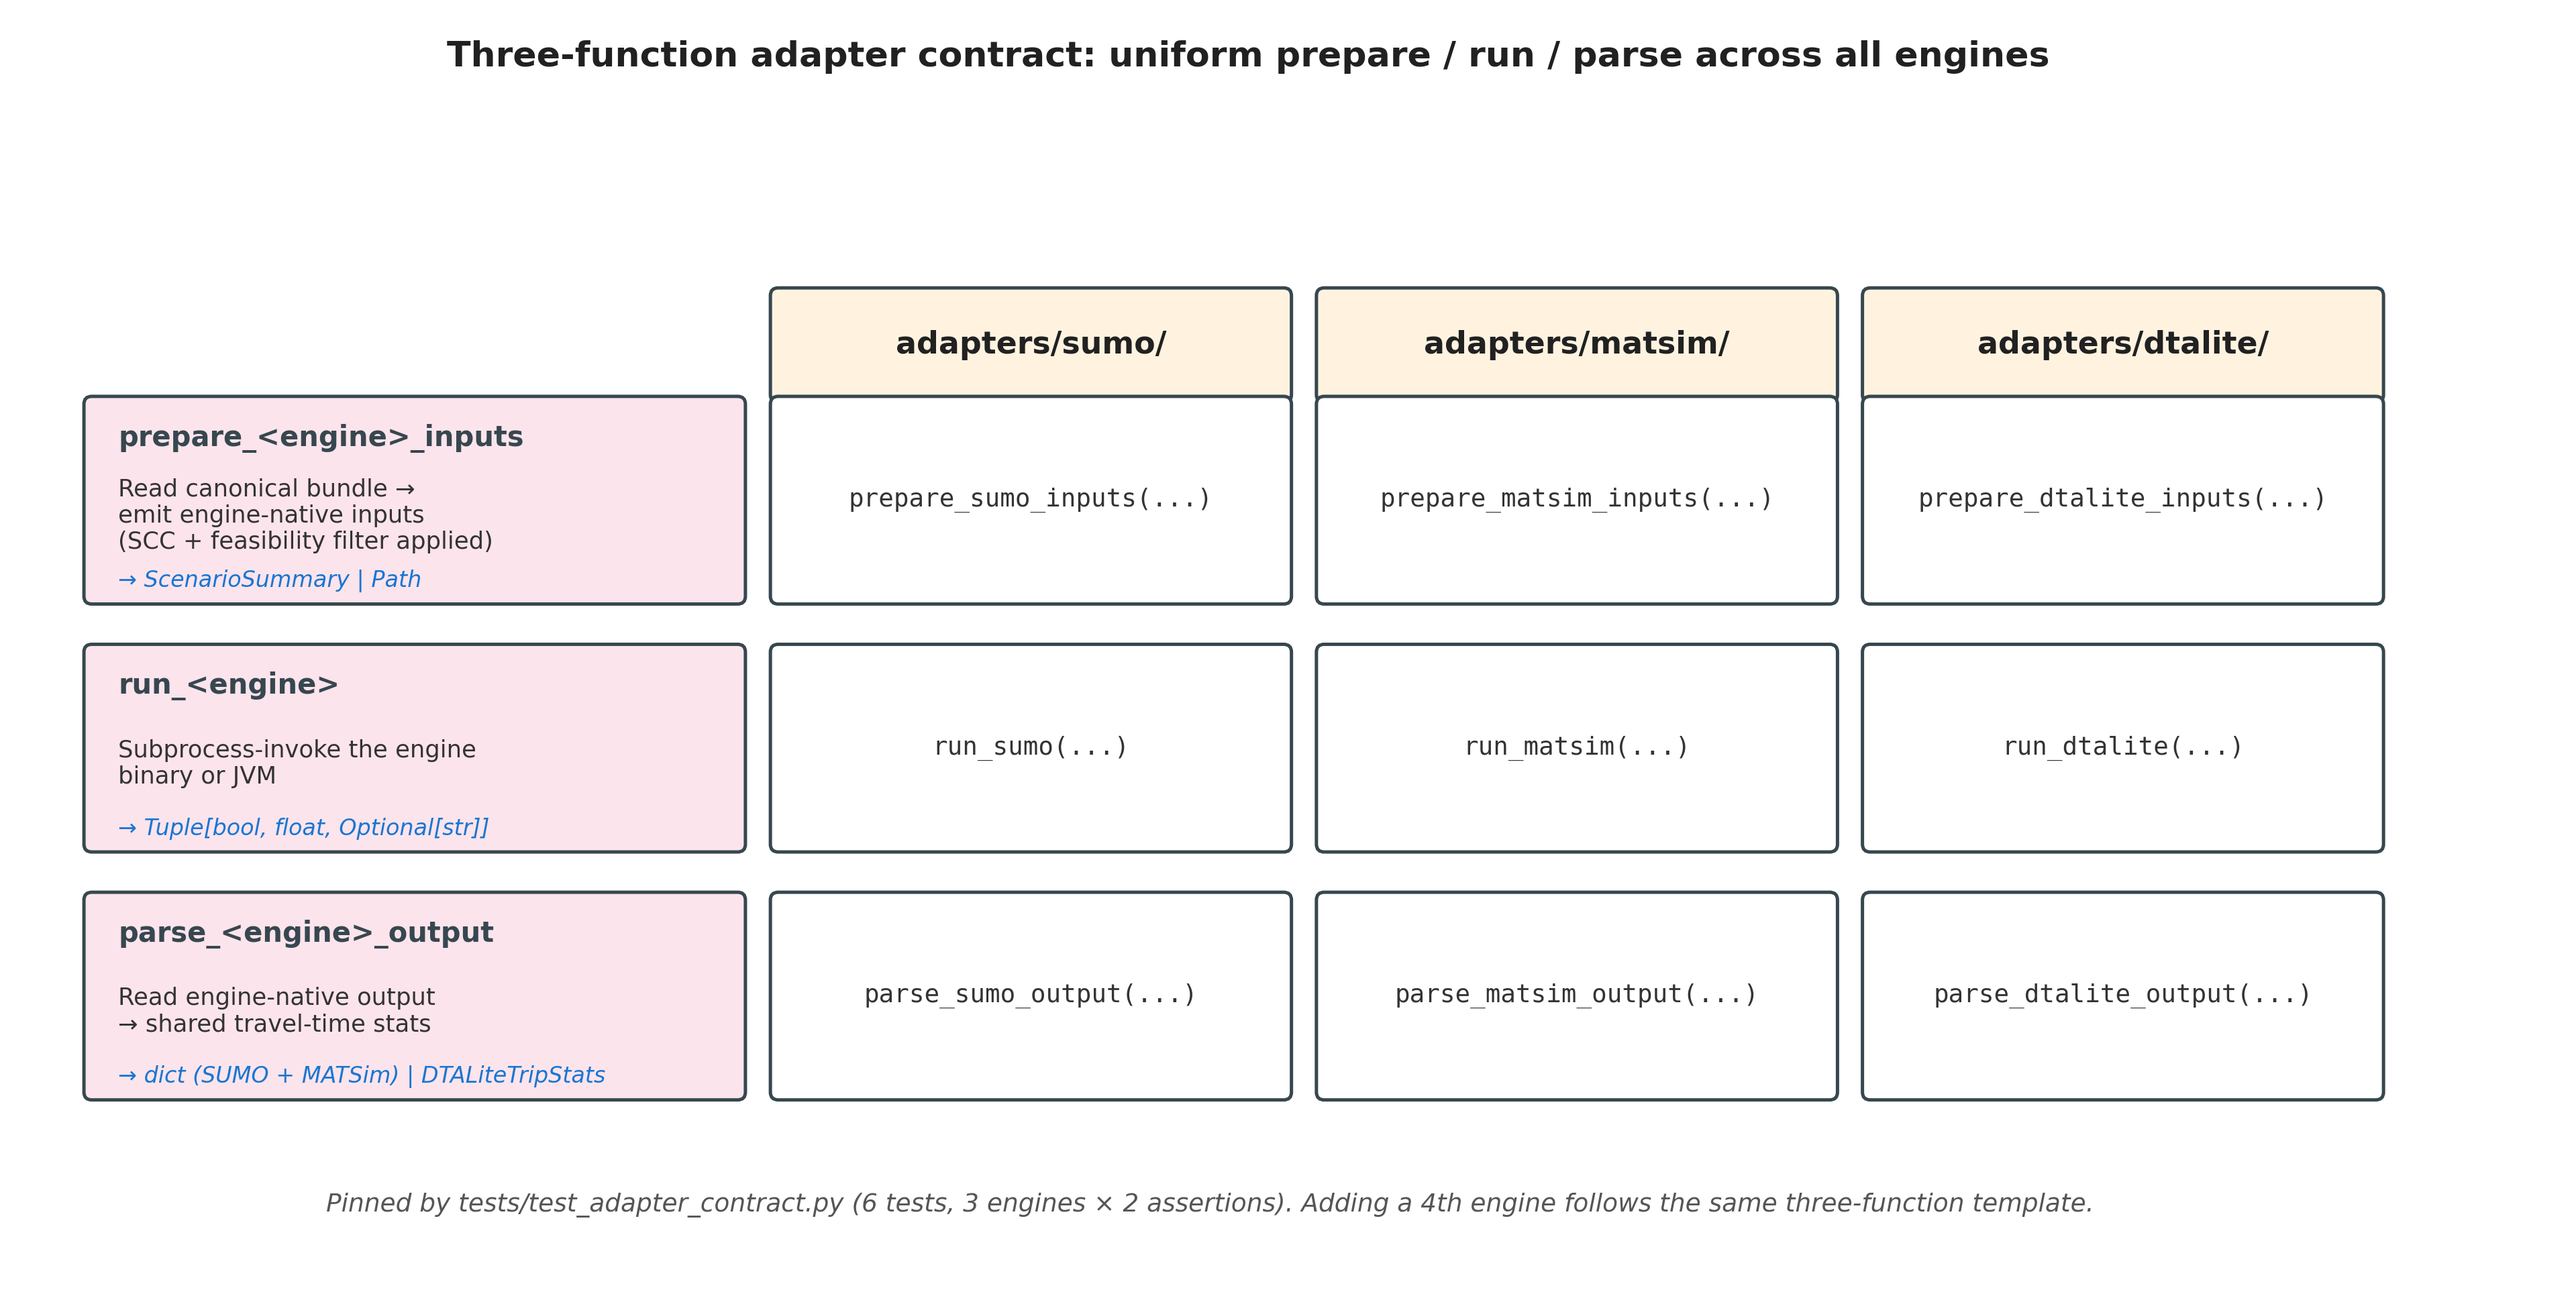
\includegraphics[keepaspectratio]{../figures/fig_3_4_adapter_contract.png}}

Figure 3.4 lays out the three-function adapter contract as a 3×3 grid:
three rows (\texttt{prepare\_\textless{}engine\textgreater{}\_inputs},
\texttt{run\_\textless{}engine\textgreater{}},
\texttt{parse\_\textless{}engine\textgreater{}\_output}) × three columns
(SUMO, MATSim, DTALite). Each cell shows the per-engine function
signature; the left labels describe the shared contract semantics and
return type. The \texttt{prepare\_} functions consume the canonical
bundle and emit engine-native inputs after applying the shared SCC +
feasibility filter and (Phase 14+) consuming canonical\_routes. The
\texttt{run\_} functions invoke the engine binary or JVM as a subprocess
and return \texttt{(success,\ runtime\_s,\ error\_msg)}. The
\texttt{parse\_} functions read engine-native outputs and return
travel-time stats --- a plain dict for SUMO + MATSim, a richer
\texttt{DTALiteTripStats} dataclass for DTALite. The contract is pinned
by \texttt{tests/test\_adapter\_contract.py} (6 tests = 3 engines × 2
assertions); adding a fourth engine follows the same template.

\subsection{Adapter Architecture}\label{341-adapter-architecture}

Each adapter implements a common operational pattern:

\begin{Shaded}
\begin{Highlighting}[]
\KeywordTok{class}\NormalTok{ SimulatorAdapter(Protocol):}
    \KeywordTok{def}\NormalTok{ prepare\_inputs(}\VariableTok{self}\NormalTok{, scenario\_path: Path, output\_dir: Path) }\OperatorTok{{-}\textgreater{}} \VariableTok{None}\NormalTok{:}
        \CommentTok{"""Convert canonical bundle to simulator{-}specific inputs."""}

    \KeywordTok{def}\NormalTok{ run\_simulation(}\VariableTok{self}\NormalTok{, config\_path: Path, }\OperatorTok{**}\NormalTok{kwargs) }\OperatorTok{{-}\textgreater{}}\NormalTok{ SimulationResult:}
        \CommentTok{"""Execute the simulator and return results."""}

    \KeywordTok{def}\NormalTok{ parse\_outputs(}\VariableTok{self}\NormalTok{, output\_dir: Path) }\OperatorTok{{-}\textgreater{}}\NormalTok{ SimulationMetrics:}
        \CommentTok{"""Extract metrics from simulator outputs."""}
\end{Highlighting}
\end{Shaded}

\textbf{Conversion guarantees:}

\begin{itemize}
\tightlist
\item
  \textbf{Deterministic}: Given the same canonical input and adapter
  version, the output is byte-identical
\item
  \textbf{Lossless (within schema)}: All canonical attributes are
  mapped; no information is dropped
\item
  \textbf{Documented}: Every mapping decision is recorded in
  \texttt{adapters/\textless{}engine\textgreater{}/MAPPING.md}
\item
  \textbf{Cross-engine vehicle alignment} (V11+): All three adapters
  source vehicle parameters from a single shared module
  \texttt{adapters/common/vehicle\_types.py}. Pre-V11 each adapter
  declared its own values inline (SUMO inherited the implicit
  \texttt{DEFAULT\_VEHTYPE}, MATSim hardcoded \texttt{length=7.5} and
  \texttt{width=1.0}), with the cross-engine equivalence undocumented
  and untested. The canonical SimForge car is now a 5.0 m sedan with a
  2.5 m gap, 1.8 m wide, 40 m/s max speed, PCE 1.0. SUMO emits
  \texttt{length="5.0"\ minGap="2.5"} (physical convention); MATSim
  emits \texttt{\textless{}length\ meter="7.5"/\textgreater{}}
  (effective-spacing convention = SUMO\textquotesingle s length +
  minGap); DTALite consumes \texttt{PCE\ =\ 1.0} (link-capacity
  convention). The equivalence is pinned by
  \texttt{tests/test\_vehicle\_types.py::TestCrossEngineEquivalence}.
  Within-bucket heterogeneity (motorcycles, taxis, freight) is post-V11
  work and remains a documented limitation.
\end{itemize}

\subsection{SUMO Adapter}\label{342-sumo-adapter}

\textbf{Simulator}: SUMO (Simulation of Urban Mobility) --- microscopic
traffic simulator modeling individual vehicles with car-following
(Krauss model) and lane-changing behavior.

\textbf{Supported modes}: Microscopic (default) and Mesoscopic
(queue-based, \textasciitilde100× faster)

\textbf{Conversion pipeline:}

\begin{verbatim}
CANONICAL                           SUMO
────────────────────────────────────────────────
network.xml  ──► nodes.nod.xml ─┐
                 edges.edg.xml ─┴─► netconvert ──► net.net.xml
demand.csv   ──► routes.rou.xml (with BFS routing)
signals.xml  ──► (embedded in net.net.xml via netconvert)
config.xml   ──► scenario.sumocfg
\end{verbatim}

\textbf{Key mapping decisions:}

\begin{longtable}[]{@{}lll@{}}
\toprule\noalign{}
Canonical & SUMO & Transformation \\
\midrule\noalign{}
\endhead
\bottomrule\noalign{}
\endlastfoot
\texttt{node\ (x,\ y)} & \texttt{node\ (x,\ y,\ type)} & x=lon, y=lat;
type defaults to \texttt{priority} \\
\texttt{link\ (from,\ to,\ length)} & \texttt{edge\ +\ lanes} & One edge
per link; numLanes, speed from canonical \\
\texttt{link.speed\_limit} & \texttt{edge.speed} & Direct copy (both in
m/s) \\
\texttt{link.lanes} & \texttt{edge.numLanes} & Direct copy \\
Trip (origin, dest) & Vehicle with route & State-aware BFS shortest path
on node graph (V5+ Phase 7) → edge sequence \\
\texttt{config.random\_seed} & \texttt{-\/-seed} CLI arg & Passed to
sumo/sumo-gui \\
\end{longtable}

\textbf{State-aware BFS routing (V5+ Phase 7)}: The SUMO adapter
computes shortest paths at conversion time (not at simulation time). For
each trip in demand.csv:

\begin{enumerate}
\def\labelenumi{\arabic{enumi}.}
\tightlist
\item
  Build the forbidden-move set from the
  \texttt{\textless{}turn\_restrictions\textgreater{}} block in
  \texttt{network.xml} via
  \texttt{pipeline/network/turn\_restrictions.build\_forbidden\_moves}.
\item
  Run state-aware BFS from \texttt{origin\_node\_id} to
  \texttt{destination\_node\_id} over \texttt{(node,\ last\_link)}
  states --- never traversing a
  \texttt{(from\_link,\ via\_node,\ to\_link)} triple in the forbidden
  set. Implemented at
  \texttt{pipeline/network/turn\_restrictions.shortest\_path\_with\_restrictions}.
\item
  Fall back to plain BFS if no restriction-respecting path exists (rare;
  SCC-feasible by construction).
\item
  Convert the node path to an edge sequence via the
  \texttt{edge\_lookup} dictionary.
\item
  Write as
  \texttt{\textless{}vehicle\ id="veh\_t0"\ depart="25200"\textgreater{}\textless{}route\ edges="l0\ l1\ l2"/\textgreater{}\textless{}/vehicle\textgreater{}}.
\end{enumerate}

The MATSim adapter uses the same state-aware BFS to pre-route every plan
and writes a
\texttt{\textless{}route\ type="links"\ start\_link="..."\ end\_link="..."\textgreater{}interior\textless{}/route\textgreater{}}
per the MATSim 15 \textbf{population\_v6} DTD (corrected from plans\_v4
in V11.2 --- plans\_v4\textquotesingle s
\texttt{\textless{}route\textgreater{}} element rejects
\texttt{type="links"} and treats text content as a node sequence;
population\_v6 supports both natively). The DTALite adapter emits a
sibling \texttt{movement.csv} with forbidden movements (capacity = 0,
penalty = 99999) but path4gmns 0.10.0 does not natively ingest it --- a
documented cross-engine asymmetry. Trips with no valid path
(disconnected OD pairs) are skipped and logged.

\textbf{Mesoscopic mode}: Activated via \texttt{-\/-mesosim} flag in
SUMO configuration. Uses queue-based link traversal instead of
car-following. Dramatically faster for large scenarios (100-1000×
speedup at 500K+ trips) with lower fidelity.

\textbf{netconvert invocation:}

\begin{Shaded}
\begin{Highlighting}[]
\ExtensionTok{netconvert} \AttributeTok{{-}{-}node{-}files}\NormalTok{ nodes.nod.xml }\DataTypeTok{\textbackslash{}}
           \AttributeTok{{-}{-}edge{-}files}\NormalTok{ edges.edg.xml }\DataTypeTok{\textbackslash{}}
           \AttributeTok{{-}{-}output{-}file}\NormalTok{ net.net.xml }\DataTypeTok{\textbackslash{}}
           \AttributeTok{{-}{-}no{-}turnarounds}
\end{Highlighting}
\end{Shaded}

\subsection{MATSim Adapter}\label{343-matsim-adapter}

\textbf{Simulator}: MATSim (Multi-Agent Transport Simulation) ---
activity-based, mesoscopic simulator modeling agents executing daily
activity plans.

\textbf{Conversion pipeline:}

\begin{verbatim}
CANONICAL                           MATSIM
────────────────────────────────────────────────
network.xml  ──► network.xml (MATSim DTD format)
demand.csv   ──► plans.xml (2-activity chains)
config.xml   ──► config.xml (MATSim config format) + vehicles.xml
\end{verbatim}

\textbf{Key mapping decisions:}

\begin{longtable}[]{@{}lll@{}}
\toprule\noalign{}
Canonical & MATSim & Notes \\
\midrule\noalign{}
\endhead
\bottomrule\noalign{}
\endlastfoot
Node (x, y) & Node with coords & Coordinates preserved as-is \\
Link & Link with freespeed, capacity &
\texttt{freespeed\ =\ speed\_limit}; capacity from lanes × 1800 \\
Trip (OD, time) & Person with 2-activity plan & home(origin) →
work(destination) \\
Mode & Leg mode & car/transit/bike mapped to MATSim modes \\
Random seed & \texttt{config/global/randomSeed} & Propagated to MATSim
config XML \\
\end{longtable}

\textbf{Demand conversion}: Each canonical trip becomes a MATSim agent
with a 2-activity plan:

\begin{Shaded}
\begin{Highlighting}[]
\NormalTok{\textless{}}\KeywordTok{person}\OtherTok{ id=}\StringTok{"person\_t0"}\NormalTok{\textgreater{}}
\NormalTok{  \textless{}}\KeywordTok{plan}\OtherTok{ selected=}\StringTok{"yes"}\NormalTok{\textgreater{}}
\NormalTok{    \textless{}}\KeywordTok{activity}\OtherTok{ type=}\StringTok{"home"}\OtherTok{ link=}\StringTok{"l\_near\_origin"}\OtherTok{ end\_time=}\StringTok{"07:00:00"}\NormalTok{/\textgreater{}}
\NormalTok{    \textless{}}\KeywordTok{leg}\OtherTok{ mode=}\StringTok{"car"}\NormalTok{/\textgreater{}}
\NormalTok{    \textless{}}\KeywordTok{activity}\OtherTok{ type=}\StringTok{"work"}\OtherTok{ link=}\StringTok{"l\_near\_destination"}\NormalTok{/\textgreater{}}
\NormalTok{  \textless{}/}\KeywordTok{plan}\NormalTok{\textgreater{}}
\NormalTok{\textless{}/}\KeywordTok{person}\NormalTok{\textgreater{}}
\end{Highlighting}
\end{Shaded}

\textbf{Single-iteration mode}: For fair comparison with SUMO, MATSim is
configured with \texttt{lastIteration=0}, disabling the iterative
replanning loop that MATSim normally uses to reach user equilibrium.

\textbf{Java/JAR detection}: The adapter auto-detects the Java runtime
and MATSim JAR location:

\begin{enumerate}
\def\labelenumi{\arabic{enumi}.}
\tightlist
\item
  Checks \texttt{JAVA\_HOME}, then \texttt{PATH}, then common install
  locations
\item
  Locates \texttt{matsim-15.0.jar} in the \texttt{lib/} directory
\item
  Constructs classpath including all dependency JARs
\end{enumerate}

\begin{longtable}[]{@{}lll@{}}
\toprule\noalign{}
Aspect & SUMO & MATSim \\
\midrule\noalign{}
\endhead
\bottomrule\noalign{}
\endlastfoot
Resolution & Vehicle-level & Agent-level \\
Demand representation & OD routes & Activity plans \\
Traffic flow & Car-following & Queue-based (mesoscopic) \\
Typical iterations & 1 & 1 (forced for fair comparison) \\
Startup overhead & \textasciitilde0.1s & \textasciitilde5-7s (JVM
warmup) \\
\end{longtable}

\subsection{DTALite Adapter}\label{344-dtalite-adapter}

\textbf{Simulator}: DTALite --- CPU-only mesoscopic Dynamic Traffic
Assignment engine distributed under Apache 2.0 license, bundled inside
the \href{https://github.com/jdlph/Path4GMNS}{\texttt{path4gmns}} Python
package. Replaces LPSim in the third-engine slot in \textbf{Version\_5}
after the LPSim integration was abandoned (see
\href{../engines/LPSIM_RETROSPECTIVE.md}{\texttt{doc/engines/LPSIM\_RETROSPECTIVE.md}}).
The selection rationale and the two ruled-out alternatives (CityFlow,
POLARIS) are documented in
\href{../engines/THIRD_ENGINE_OPTIONS.md}{\texttt{doc/engines/THIRD\_ENGINE\_OPTIONS.md}}.

\textbf{Conversion} (Canonical → GMNS schema):

\begin{longtable}[]{@{}lll@{}}
\toprule\noalign{}
File & Canonical & DTALite (GMNS) \\
\midrule\noalign{}
\endhead
\bottomrule\noalign{}
\endlastfoot
Nodes & \texttt{network.xml}
\texttt{\textless{}node\ id="n123"\ x="…"\ y="…"/\textgreater{}} &
\texttt{node.csv} columns
\texttt{node\_id,\ zone\_id,\ x\_coord,\ y\_coord,\ production,\ attraction} \\
Edges & \texttt{network.xml}
\texttt{\textless{}link\ id="l456"\ from="n10"\ to="n11"\ length="120.5"\ speed\_limit="13.9"\ lanes="2"/\textgreater{}}
& \texttt{link.csv} columns
\texttt{link\_id,\ from\_node\_id,\ to\_node\_id,\ length\ (km),\ lanes,\ free\_speed\ (km/h),\ capacity,\ link\_type,\ VDF\_fftt1,\ VDF\_alpha1,\ VDF\_beta1}
(m → km, m/s × 3.6 → km/h) \\
Demand & \texttt{demand.csv}
\texttt{trip\_id,\ origin\_node\_id,\ destination\_node\_id,\ departure\_time\_s,\ mode}
& \texttt{demand.csv} columns
\texttt{o\_zone\_id,\ d\_zone\_id,\ volume} (trips aggregated by OD
pair) \\
Config & \texttt{config.xml}
\texttt{\textless{}time\ start\_time\_s="25200"\ end\_time\_s="28800"/\textgreater{}}
& \texttt{settings.csv} (\texttt{{[}demand\_period{]}} AM 0700\_0800) +
\texttt{settings.yml} mirror for the path4gmns Python wrapper \\
\end{longtable}

\textbf{Demand-driven zoning}: DTALite\textquotesingle s UE assignment
iterates over zones, running label-correcting shortest-path from each
zone in every outer iteration. Treating every node as a zone (the naive
approach) produced 20,058-zone runs that took minutes per outer
iteration on chicago\_1k\_car. The adapter therefore promotes only nodes
that appear as origin or destination in the demand to GMNS zones
(\textasciitilde1,800 zones for chicago\_1k\_car); transit-only
intersections retain network connectivity but are skipped in the UE
loop. Runtime drops from "minutes" to \textasciitilde5 seconds at the
bundled scenario size.

\textbf{Fidelity trade-off --- departure timing}:
DTALite\textquotesingle s GMNS demand format does not include a per-trip
departure column; trips are aggregated by (origin, destination) into a
count \texttt{volume}. Departures are distributed uniformly inside the
\texttt{{[}demand\_period{]}} window (default 0700-0800 --- controlled
by \texttt{DTALiteConfig}). The canonical \texttt{departure\_time\_s}
precision available to SUMO and MATSim is therefore not exposed to
DTALite. This is the single cleanest difference between the three
engines from a demand-modeling perspective and is documented in
\texttt{adapters/dtalite/MAPPING.md} for full audit trail.

\textbf{Determinism}: DTALite is fully deterministic. The UE algorithm
(Method of Successive Averages / Frank-Wolfe) iterates in fixed order
with no atomic reductions and no GPU non-determinism. R-score is
expected to be 1.0 across N=5 repeats with the same inputs, matching
SUMO mesoscopic and MATSim with \texttt{lastIteration=0}. (This
determinism is one of the technical reasons DTALite was preferred over
LPSim, whose \texttt{atomicAdd} GPU reductions would have forced an
explanatory footnote on every reproducibility number --- see
\texttt{LPSIM\_RETROSPECTIVE.md} §5.)

\textbf{Binary discovery}: \texttt{is\_dtalite\_available()} checks both
that \texttt{path4gmns} is importable AND that the platform-specific
bundled binary (\texttt{DTALiteMM\_arm.dylib} /
\texttt{DTALiteMM\_x86.dylib} / \texttt{DTALiteMM.so} /
\texttt{DTALiteMM.dll}) exists in the package\textquotesingle s
\texttt{bin/} directory. With path4gmns not installed,
\texttt{run\_dtalite()} returns a clean \texttt{RunResult} failure with
the install command (\texttt{uv\ pip\ install\ path4gmns}) --- no silent
fallback (the failure mode that motivated dropping QarSUMO).

\textbf{Implementation note} --- DTALiteClassic vs DTALiteMultimodal:
path4gmns 0.10.0 ships two DTALite binaries. The adapter calls
\texttt{DTALiteClassic} (mode 1 = path-based UE), not the newer
\texttt{DTALiteMultimodal} wrapper. The multimodal binary has a
regression demanding a \texttt{mode\_type.csv} schema upstream has not
published --- even path4gmns\textquotesingle s own bundled samples fail
with
\texttt{{[}ERROR{]}\ File\ mode\_type\ does\ not\ have\ information}
when invoked fresh. Full implementation note in
\texttt{adapters/dtalite/MAPPING.md}.

\textbf{Performance expectation}: at SimForge scenario sizes (1k--500k
trips, ≤500k nodes) DTALite is comparable to MATSim in wallclock ---
slower than SUMO meso, faster than SUMO micro at scale. The thesis claim
is paradigm spread (microscopic + queue-based agent + DTA equilibrium),
not raw speedup; see \texttt{doc/engines/ENGINE\_COMPARISON.md} §3 for
the per-tier wallclock estimates.

\subsection{Adapter Determinism}\label{345-adapter-determinism}

All adapters enforce deterministic output through:

\begin{enumerate}
\def\labelenumi{\arabic{enumi}.}
\tightlist
\item
  \textbf{Sorted iteration}: All XML elements emitted in sorted order
  (by node ID, link ID, etc.) --- avoids hash-set iteration order
  differences
\item
  \textbf{Fixed random seeds}: The canonical \texttt{random\_seed} from
  config.xml is propagated to all simulator-level random seed parameters
\item
  \textbf{Version pinning}: Adapter code is versioned alongside the
  framework; simulator versions are recorded in metadata
\item
  \textbf{Hash verification}: Post-conversion, the adapter can
  re-validate that canonical inputs haven\textquotesingle t drifted
  since scenario generation
\end{enumerate}

\begin{center}\rule{0.5\linewidth}{0.5pt}\end{center}

\section{Execution Harness}\label{35-execution-harness}

\subsection{Run Specification
Schema}\label{351-run-specification-schema}

Benchmark runs are defined via YAML runspec files that specify the
experimental matrix:

\begin{Shaded}
\begin{Highlighting}[]
\FunctionTok{name}\KeywordTok{:}\AttributeTok{ stress\_test}
\FunctionTok{description}\KeywordTok{:}\AttributeTok{ End{-}to{-}end stress test across all engines and modes.}
\FunctionTok{output\_dir}\KeywordTok{:}\AttributeTok{ runs/benchmark\_small}

\FunctionTok{runs}\KeywordTok{:}
\AttributeTok{  }\KeywordTok{{-}}\AttributeTok{ }\FunctionTok{scenario\_id}\KeywordTok{:}\AttributeTok{ chicago\_1k\_car}
\AttributeTok{    }\FunctionTok{scenario\_path}\KeywordTok{:}\AttributeTok{ scenarios/chicago\_1k\_car}
\AttributeTok{    }\FunctionTok{engine}\KeywordTok{:}\AttributeTok{ sumo}
\AttributeTok{    }\FunctionTok{mode}\KeywordTok{:}\AttributeTok{ mesoscopic}
\AttributeTok{    }\FunctionTok{repeats}\KeywordTok{:}\AttributeTok{ }\DecValTok{3}
\AttributeTok{    }\FunctionTok{seed}\KeywordTok{:}\AttributeTok{ }\DecValTok{42}
\AttributeTok{    }\FunctionTok{timeout\_s}\KeywordTok{:}\AttributeTok{ }\DecValTok{300}

\AttributeTok{  }\KeywordTok{{-}}\AttributeTok{ }\FunctionTok{scenario\_id}\KeywordTok{:}\AttributeTok{ chicago\_1k\_car}
\AttributeTok{    }\FunctionTok{scenario\_path}\KeywordTok{:}\AttributeTok{ scenarios/chicago\_1k\_car}
\AttributeTok{    }\FunctionTok{engine}\KeywordTok{:}\AttributeTok{ matsim}
\AttributeTok{    }\FunctionTok{mode}\KeywordTok{:}\AttributeTok{ mesoscopic}
\AttributeTok{    }\FunctionTok{repeats}\KeywordTok{:}\AttributeTok{ }\DecValTok{2}
\AttributeTok{    }\FunctionTok{seed}\KeywordTok{:}\AttributeTok{ }\DecValTok{42}
\AttributeTok{    }\FunctionTok{timeout\_s}\KeywordTok{:}\AttributeTok{ }\DecValTok{600}
\end{Highlighting}
\end{Shaded}

\textbf{RunConfig fields:}

\begin{longtable}[]{@{}lll@{}}
\toprule\noalign{}
Field & Type & Description \\
\midrule\noalign{}
\endhead
\bottomrule\noalign{}
\endlastfoot
\texttt{scenario\_id} & string & Human-readable scenario identifier \\
\texttt{scenario\_path} & string & Path to canonical scenario bundle \\
\texttt{engine} & string & Simulator: \texttt{sumo}, \texttt{matsim},
\texttt{dtalite} \\
\texttt{mode} & enum & \texttt{microscopic} or \texttt{mesoscopic} \\
\texttt{repeats} & int & Number of repeated runs (for reproducibility
analysis) \\
\texttt{seed} & int & Base seed (incremented per repeat: 42, 43, 44) \\
\texttt{timeout\_s} & int & Maximum wall-clock time per run \\
\end{longtable}

\textbf{SimulationMode enum:}

\begin{Shaded}
\begin{Highlighting}[]
\KeywordTok{class}\NormalTok{ SimulationMode(}\BuiltInTok{str}\NormalTok{, Enum):}
\NormalTok{    MICROSCOPIC }\OperatorTok{=} \StringTok{"microscopic"}  \CommentTok{\# Car{-}following + lane{-}changing (accurate, slow)}
\NormalTok{    MESOSCOPIC }\OperatorTok{=} \StringTok{"mesoscopic"}    \CommentTok{\# Queue{-}based edge traversal (fast, \textasciitilde{}100× speedup)}
\end{Highlighting}
\end{Shaded}

\subsection{Benchmark Execution
Pipeline}\label{352-benchmark-execution-pipeline}

The \texttt{BenchmarkHarness} orchestrates the full execution lifecycle:

\begin{verbatim}
For each (scenario, engine, mode, seed):
    1. Validate canonical bundle  ──► abort if invalid
    2. Prepare simulator inputs   ──► adapter.prepare_inputs()
    3. Execute simulation         ──► adapter.run_simulation()
    4. Collect raw outputs        ──► tripinfo.xml, summary.xml, etc.
    5. Compute metrics            ──► adapter.parse_outputs()
    6. Record RunResult           ──► JSON serializable
\end{verbatim}

\textbf{Progress tracking}: The \texttt{StickyProgress} bar displays
real-time progress with completion ratio, ✓/✗ counts, elapsed clock, and
a Braille spinner heartbeat (V11.2+ removed the ETA estimate ---
SimForge cells are heterogeneous, so a running-mean ETA swings between
unhelpful extremes):

\begin{verbatim}
[████████████████████░░░░░░░░░░░░░░░░░░░░] 52.3%  ⠼  47/90 runs  ✓45 ✗2  elapsed 12m 30s
\end{verbatim}

\textbf{Output structure:}

\begin{verbatim}
runs/
└── benchmark_20250615_143022/
    ├── chicago_1k_car_sumo_meso_seed42/
    │   ├── net.net.xml
    │   ├── routes.rou.xml
    │   ├── scenario.sumocfg
    │   └── output/
    │       ├── tripinfo.xml
    │       └── summary.xml
    ├── chicago_1k_car_matsim_meso_seed42/
    │   ├── network.xml
    │   ├── plans.xml
    │   ├── config.xml
    │   └── output/
    │       └── output_events.xml.gz
    └── benchmark_results_<runspec>.json
\end{verbatim}

\subsection{Result Aggregation}\label{353-result-aggregation}

All run results are serialized to
\texttt{benchmark\_results\_\textless{}runspec\textgreater{}.json}:

\begin{Shaded}
\begin{Highlighting}[]
\FunctionTok{\{}
  \DataTypeTok{"runspec\_name"}\FunctionTok{:} \StringTok{"stress\_test"}\FunctionTok{,}
  \DataTypeTok{"started\_at"}\FunctionTok{:} \StringTok{"2026{-}04{-}19T02:05:28+00:00"}\FunctionTok{,}
  \DataTypeTok{"completed\_at"}\FunctionTok{:} \StringTok{"2026{-}04{-}19T02:06:19+00:00"}\FunctionTok{,}
  \DataTypeTok{"total\_runs"}\FunctionTok{:} \DecValTok{22}\FunctionTok{,}
  \DataTypeTok{"successful\_runs"}\FunctionTok{:} \DecValTok{22}\FunctionTok{,}
  \DataTypeTok{"failed\_runs"}\FunctionTok{:} \DecValTok{0}\FunctionTok{,}
  \DataTypeTok{"results"}\FunctionTok{:} \OtherTok{[}
    \FunctionTok{\{}
      \DataTypeTok{"scenario"}\FunctionTok{:} \StringTok{"chicago\_1k\_car"}\FunctionTok{,}
      \DataTypeTok{"engine"}\FunctionTok{:} \StringTok{"sumo"}\FunctionTok{,}
      \DataTypeTok{"mode"}\FunctionTok{:} \StringTok{"meso"}\FunctionTok{,}
      \DataTypeTok{"seed"}\FunctionTok{:} \DecValTok{42}\FunctionTok{,}
      \DataTypeTok{"status"}\FunctionTok{:} \StringTok{"success"}\FunctionTok{,}
      \DataTypeTok{"runtime\_s"}\FunctionTok{:} \FloatTok{0.279}\FunctionTok{,}
      \DataTypeTok{"metrics"}\FunctionTok{:} \FunctionTok{\{}
        \DataTypeTok{"travel\_time"}\FunctionTok{:} \FunctionTok{\{}
          \DataTypeTok{"mean"}\FunctionTok{:} \FloatTok{204.18}\FunctionTok{,}
          \DataTypeTok{"p95"}\FunctionTok{:} \FloatTok{406.0}\FunctionTok{,}
          \DataTypeTok{"trip\_count"}\FunctionTok{:} \DecValTok{996}
        \FunctionTok{\}}
      \FunctionTok{\}}
    \FunctionTok{\}}
  \OtherTok{]}
\FunctionTok{\}}
\end{Highlighting}
\end{Shaded}

\begin{center}\rule{0.5\linewidth}{0.5pt}\end{center}

\section{Evaluation Metrics}\label{36-evaluation-metrics}

\pandocbounded{
\includegraphics[keepaspectratio]{../figures/fig_3_6_fairness_audit_flow.png}}

Figure 3.6 walks through the cross-engine fairness audit
(\texttt{evaluation/audit\_fairness.py}) as a vertical flow. Input is a
run directory containing per-engine cells. The audit then runs five
questions in order, each producing a verdict line in the audit output:
\textbf{Q1} (mandatory) --- byte-identical feasibility verdicts across
all engines; \textbf{Q2} (mandatory) --- byte-identical SCC node + link
counts; \textbf{Q3} (mandatory) --- every engine simulated the same
trip-count target; \textbf{Q4} (informational) --- cross-engine mean-TT
comparison (the paradigm-divergence signal that drives §5.6.2);
\textbf{Q5} (informational) --- V5+ demand-composition tally. Q1-Q3 are
the \emph{fairness contract} --- they must PASS for the cross-engine
comparison to be attributable to engine paradigm rather than input
asymmetry. Q4 + Q5 are the interpretive readouts that make the
fairness-contract guarantee actionable for the chapter-5
paradigm-divergence narrative.

\subsection{Metric Categories}\label{361-metric-categories}

The evaluation framework measures three orthogonal quality dimensions:

\begin{longtable}[]{@{}lll@{}}
\toprule\noalign{}
Dimension & Question & Metrics \\
\midrule\noalign{}
\endhead
\bottomrule\noalign{}
\endlastfoot
\textbf{Fidelity} & How closely do simulators agree with each other? &
RMSE, GEH, KS statistic \\
\textbf{Scalability} & How efficiently does each simulator use compute
resources? & Runtime, throughput, SRT \\
\textbf{Reproducibility} & How consistent are results across repeated
runs? & Reproducibility index \(R\) \\
\end{longtable}

\subsection{Fidelity Metrics}\label{362-fidelity-metrics}

\textbf{Root Mean Square Error (RMSE):}

\[\text{RMSE} = \sqrt{\frac{1}{n}\sum_{i=1}^{n}(y_i - \hat{y}_i)^2}\]

Applied to link-level traffic counts or travel times across two
simulators. Lower RMSE indicates closer agreement. Units match the input
(seconds for travel time, vehicles for counts).

\textbf{GEH Statistic} (Geoffrey E. Havers):

\[\text{GEH} = \sqrt{\frac{2(M - C)^2}{M + C}}\]

where \(M\) is the modeled value and \(C\) is the comparison/observed
value. Standard in traffic engineering (UK DfT, FHWA):

\begin{longtable}[]{@{}lll@{}}
\toprule\noalign{}
GEH Range & Interpretation & Action \\
\midrule\noalign{}
\endhead
\bottomrule\noalign{}
\endlastfoot
\textless{} 5 & Acceptable fit & No action needed \\
5 -- 10 & Warrants investigation & Check individual links \\
\textgreater{} 10 & Poor fit & Model needs revision \\
\end{longtable}

The implementation computes per-link GEH and reports both the
\textbf{mean GEH} and the \textbf{percentage of links with GEH
\textless{} 5} (the industry-standard acceptance criterion).

\textbf{Kolmogorov-Smirnov Statistic:}

\[D = \sup_x |F_1(x) - F_2(x)|\]

Compares the empirical cumulative distribution functions (CDFs) of
travel time distributions from two simulators. Critical value at
significance level \(\alpha = 0.05\):

\[D_{\text{crit}} = 1.36 \sqrt{\frac{n_1 + n_2}{n_1 \cdot n_2}}\]

If \(D > D_{\text{crit}}\), the distributions are statistically
different at the 5\% level.

\subsection{Scalability Metrics}\label{363-scalability-metrics}

\textbf{Wall-clock runtime}: Measured via \texttt{time.perf\_counter()}
context manager for nanosecond precision:

\begin{Shaded}
\begin{Highlighting}[]
\KeywordTok{class}\NormalTok{ SimulationTimer:}
    \KeywordTok{def} \FunctionTok{\_\_enter\_\_}\NormalTok{(}\VariableTok{self}\NormalTok{):}
        \VariableTok{self}\NormalTok{.start\_time }\OperatorTok{=}\NormalTok{ time.perf\_counter()}
        \ControlFlowTok{return} \VariableTok{self}
    \KeywordTok{def} \FunctionTok{\_\_exit\_\_}\NormalTok{(}\VariableTok{self}\NormalTok{, }\OperatorTok{*}\NormalTok{args):}
        \VariableTok{self}\NormalTok{.elapsed\_seconds }\OperatorTok{=}\NormalTok{ time.perf\_counter() }\OperatorTok{{-}} \VariableTok{self}\NormalTok{.start\_time}
\end{Highlighting}
\end{Shaded}

\textbf{Throughput:}

\[\text{Throughput} = \frac{\text{vehicles completed}}{\text{wall-clock seconds}}\]

Units: vehicles/second. Higher is better. Enables direct comparison
across hardware.

\textbf{Simulated-to-Real-Time ratio (SRT):}

\[\text{SRT} = \frac{T_\text{simulated}}{T_\text{wall-clock}}\]

SRT \textgreater{} 1 means the simulator is faster than real time. SRT =
10 means 1 hour of traffic simulated in 6 minutes.

\textbf{Normalized throughput} (when hardware info available):

\[\text{Throughput}_\text{core} = \frac{\text{Throughput}}{\text{CPU cores}}\]

\[\text{Throughput}_\text{watt} = \frac{\text{Throughput}}{\text{TDP (watts)}}\]

\textbf{Hardware detection}: The framework auto-detects CPU model, core
count, and memory via platform APIs.

\subsection{Reproducibility
Metric}\label{364-reproducibility-metric}

\textbf{Coefficient of Reproducibility:}

\[R = 1 - \frac{\sigma}{\mu}\]

where \(\sigma\) is standard deviation and \(\mu\) is mean of a KPI
across repeated runs with different random seeds.

\begin{longtable}[]{@{}ll@{}}
\toprule\noalign{}
\(R\) Range & Interpretation \\
\midrule\noalign{}
\endhead
\bottomrule\noalign{}
\endlastfoot
\(R \geq 0.99\) & Excellent (near-deterministic) \\
\(0.95 \leq R < 0.99\) & Very good \\
\(0.90 \leq R < 0.95\) & Good \\
\(0.80 \leq R < 0.90\) & Acceptable \\
\(0.50 \leq R < 0.80\) & Marginal \\
\(R < 0.50\) & Poor \\
\end{longtable}

\textbf{Multi-KPI analysis}: The \texttt{MultiKPIReproducibility} class
computes \(R\) across multiple KPIs (mean travel time, p95 travel time,
throughput, etc.) and reports the \textbf{overall reproducibility} as
the average \(R\) across all KPIs.

\textbf{Edge case handling:}

\begin{itemize}
\tightlist
\item
  All values identical → \(R = 1.0\) (perfect reproducibility)
\item
  Mean near zero → special handling to avoid division instability
\item
  Fewer than 2 runs → error (meaningless without repetition)
\end{itemize}

\subsection{Travel Time
Extraction}\label{365-travel-time-extraction}

The \texttt{travel\_time} module parses simulator-specific output files
to extract trip-level metrics:

\textbf{SUMO tripinfo.xml parsing:}

\begin{Shaded}
\begin{Highlighting}[]
\NormalTok{\textless{}}\KeywordTok{tripinfo}\OtherTok{ id=}\StringTok{"veh\_t0"}\OtherTok{ depart=}\StringTok{"25200.00"}\OtherTok{ departDelay=}\StringTok{"0.00"}
\OtherTok{          arrival=}\StringTok{"25445.30"}\OtherTok{ duration=}\StringTok{"245.30"}\OtherTok{ routeLength=}\StringTok{"3240.1"}\NormalTok{/\textgreater{}}
\end{Highlighting}
\end{Shaded}

Extracted fields: \texttt{duration} (travel time in seconds) for each
completed trip.

\textbf{Computed statistics:}

\begin{longtable}[]{@{}ll@{}}
\toprule\noalign{}
Statistic & Formula \\
\midrule\noalign{}
\endhead
\bottomrule\noalign{}
\endlastfoot
Mean travel time & \(\bar{t} = \frac{1}{n}\sum_i t_i\) \\
P95 travel time & 95th percentile of sorted durations \\
Trip completion count & Number of trips with arrival time \textless{}
end\_time \\
\end{longtable}

\begin{center}\rule{0.5\linewidth}{0.5pt}\end{center}

\section{Implementation Quality}\label{37-implementation-quality}

\subsection{Test Suite}\label{371-test-suite}

The framework includes \textbf{\textasciitilde639 tests} with all 5
bundles generated (\texttt{chicago\_1k\_car}, \texttt{nyc\_10k\_car},
\texttt{la\_50k\_car}, \texttt{chicago\_200k\_car},
\texttt{nyc\_500k\_car}). The base count is roughly 450 tests plus 36
parametrized integrity tests per bundle in \texttt{scenarios/}. Phase 14
additions (\texttt{test\_canonical\_routes.py} byte-identity guards) and
Phase 14.13 additions (\texttt{test\_run\_benchmark.py} cache-hoist
guards) account for most of the count growth over the pre-Phase-14
baseline of \textasciitilde574 tests.

\begin{longtable}[]{@{}lll@{}}
\toprule\noalign{}
Test Module & Tests & What It Validates \\
\midrule\noalign{}
\endhead
\bottomrule\noalign{}
\endlastfoot
\texttt{test\_adapter\_determinism.py} & 8 & Byte-identical outputs from
identical inputs \\
\texttt{test\_sumo\_adapter.py} & 4 & SUMO conversion: network, routes,
config \\
\texttt{test\_matsim\_adapter.py} & 26 & MATSim adapter (incl. Phase
12.1 route-text format pin) \\
\texttt{test\_fidelity\_metrics.py} & 21 & RMSE, GEH, KS computation
correctness \\
\texttt{test\_metrics\_travel\_time.py} & 2 & SUMO tripinfo parsing \\
\texttt{test\_reproducibility\_metrics.py} & 15 & R-index computation,
edge cases, interpretation \\
\texttt{test\_scalability\_metrics.py} & 8 & Timer, throughput, hardware
detection \\
\texttt{test\_validator.py} & 2 & Bundle validation: valid and invalid
bundles \\
\texttt{test\_scenario\_data\_integrity.py} & 36 × N & 7 classes × 36
tests/scenario × N bundles in \texttt{scenarios/} (108 for 3 tracked,
180 for all 5) \\
\texttt{test\_pipeline\_e2e.py} & 20 & Bad data detection, routing,
adapter robustness \\
\texttt{test\_scc.py} & 14 & Iterative Kosaraju + parsing \\
\texttt{test\_feasibility.py} & 19 & Shared cross-engine trip filter +
V5 mode-aware feasibility \\
\texttt{test\_analyze\_benchmark.py} & 24 & Mode-aware grouping + Phase
10 demand composition table \\
\texttt{test\_audit\_fairness.py} & 40 & Q1--Q5 audit helpers + 5-layout
detector (Phase 12+ mode-segmented + back-compat fallbacks) \\
\texttt{test\_run\_benchmark.py} (Phase 12+) & 12 & BenchmarkHarness
explicit-output, prep-cache, bundle-hash invalidation, scoped\_base
collapse (Phase 12.2) \\
\texttt{test\_confidence.py} & 18 & Student\textquotesingle s-t 95 \% CI
core + edge cases \\
\texttt{test\_osm\_fetch.py} & 20 & OSM/Overpass fetch (mocked), bbox
validation, cache pin \\
\texttt{test\_demand\_generators.py} & 21 & Uniform/gravity/peak-hour
generators, SCC restriction \\
\texttt{test\_demand\_composition.py} (V5+ Phase 10) & 7 &
\texttt{purpose} column tally, AM/PM peak split, pre-V5 graceful
no-op \\
\texttt{test\_parse\_model\_file.py} & 27 & ModelGen parser + V5 Phase 5
JWTRNS mapping + Phase 9 HBSchool helpers \\
\texttt{test\_turn\_restrictions.py} (V5+ Phase 7) & 17 & OSM
restriction parser, forbidden-move builder, state-aware BFS, DTALite
movement.csv \\
\texttt{test\_vehicle\_types.py} (V5+ Phase 11) & 19 & Canonical car
constants, SUMO/MATSim XML emission, cross-engine equivalence \\
\texttt{test\_dtalite\_adapter.py} & 46 & DTALite adapter: writers,
settings, demand-driven zoning, determinism, output parsing, end-to-end
smoke \\
\texttt{test\_engine\_smoke.py} & 4 & Real-binary smoke on
SUMO/MATSim/DTALite \\
\texttt{test\_adapter\_contract.py} (audit) & 6 & Three-function adapter
contract regression guard (prepare/run/parse across
SUMO+MATSim+DTALite) \\
\end{longtable}

\textbf{All \textasciitilde639 tests passing} with all 5 bundles
generated, as of the Phase 14.13 cache-hoist landing (commit
\texttt{db8d786}, 2026-05-19). Marker registry in
\texttt{pyproject.toml}; shared fixtures in \texttt{tests/conftest.py}.
Line coverage sits at \textbf{76 \%} across the adapter, pipeline, and
evaluation packages; the local gate enforces ≥70 \% via
\texttt{pytest\ -\/-cov\ -\/-cov-fail-under=70}.

\subsection{Determinism
Guarantees}\label{372-determinism-guarantees}

\begin{longtable}[]{@{}ll@{}}
\toprule\noalign{}
Mechanism & What It Ensures \\
\midrule\noalign{}
\endhead
\bottomrule\noalign{}
\endlastfoot
Fixed random seeds & All stochastic processes seeded via config.xml
\texttt{random\_seed} \\
Sorted outputs & All XML/CSV files use sorted iteration over
sets/dicts \\
SHA-256 hashes & Manifest checksums detect any input drift \\
Version pinning & \texttt{requirements.txt} specifies exact package
versions \\
Per-bundle toolchain capture &
\texttt{generation\_metadata.json::toolchain} records the Python and dep
versions that built each bundle \\
Deterministic BFS & Adapter routing uses sorted adjacency lists for
tie-breaking \\
Schedule-first hybrid (demand) & PUMS-derived workplace destinations are
deterministic per (modelgen, network, seed) triple \\
\end{longtable}

\textbf{Cross-platform reproducibility (verified).} Generation produces
byte-identical \texttt{demand.csv} and \texttt{signals.xml} across
(Apple Silicon ARM64, macOS, Python 3.13.2, osmnx 2.0.7) and (x86\_64,
RHEL Pitzer, Python 3.12.4, osmnx 2.1.0), verified empirically on the
\texttt{la\_50k\_car} bundle (50K LA car + transit + bike trips,
06:00--10:00, 10 km radius, seed 42). The \texttt{network.xml} file
itself differs in MD5 across the two architectures because the lxml
serialization is version-dependent (attribute ordering, float-precision
rendering); the semantic content (node IDs, edge
\texttt{from}/\texttt{to} pairs, attributes, SCC membership) is
identical, as proven by both downstream artefacts being byte-equal ---
they reference network node IDs by string, so any drift would have
propagated. The verification recipe and reference MD5 hashes are
documented in
\href{../REPRODUCING.md\#cross-platform-reproducibility-verified}{doc/REPRODUCING.md
§Cross-Platform Reproducibility}. At the level the simulators care about
(the canonical \texttt{demand.csv} and \texttt{signals.xml} consumed by
every adapter), generation is fully cross-platform reproducible.

\subsection{Error Handling}\label{373-error-handling}

\begin{itemize}
\tightlist
\item
  \textbf{Graceful fallback}: MATSim adapter detects missing Java and
  reports an actionable error rather than producing empty outputs
\item
  \textbf{Informative errors}: Demand generation provides specific
  guidance when model file lacks data for the target city
\item
  \textbf{Timeout protection}: Each simulation run has a configurable
  timeout to prevent HPC job hangs
\item
  \textbf{Progress tracking}: Real-time progress bars with ETA prevent
  silent failures in long benchmark runs
\end{itemize}

\section{Canonical-Routes BFS Deduplication and Parallelization
(Phase
14)}\label{38-canonical-routes-bfs-deduplication-and-parallelization-phase-14}

\pandocbounded{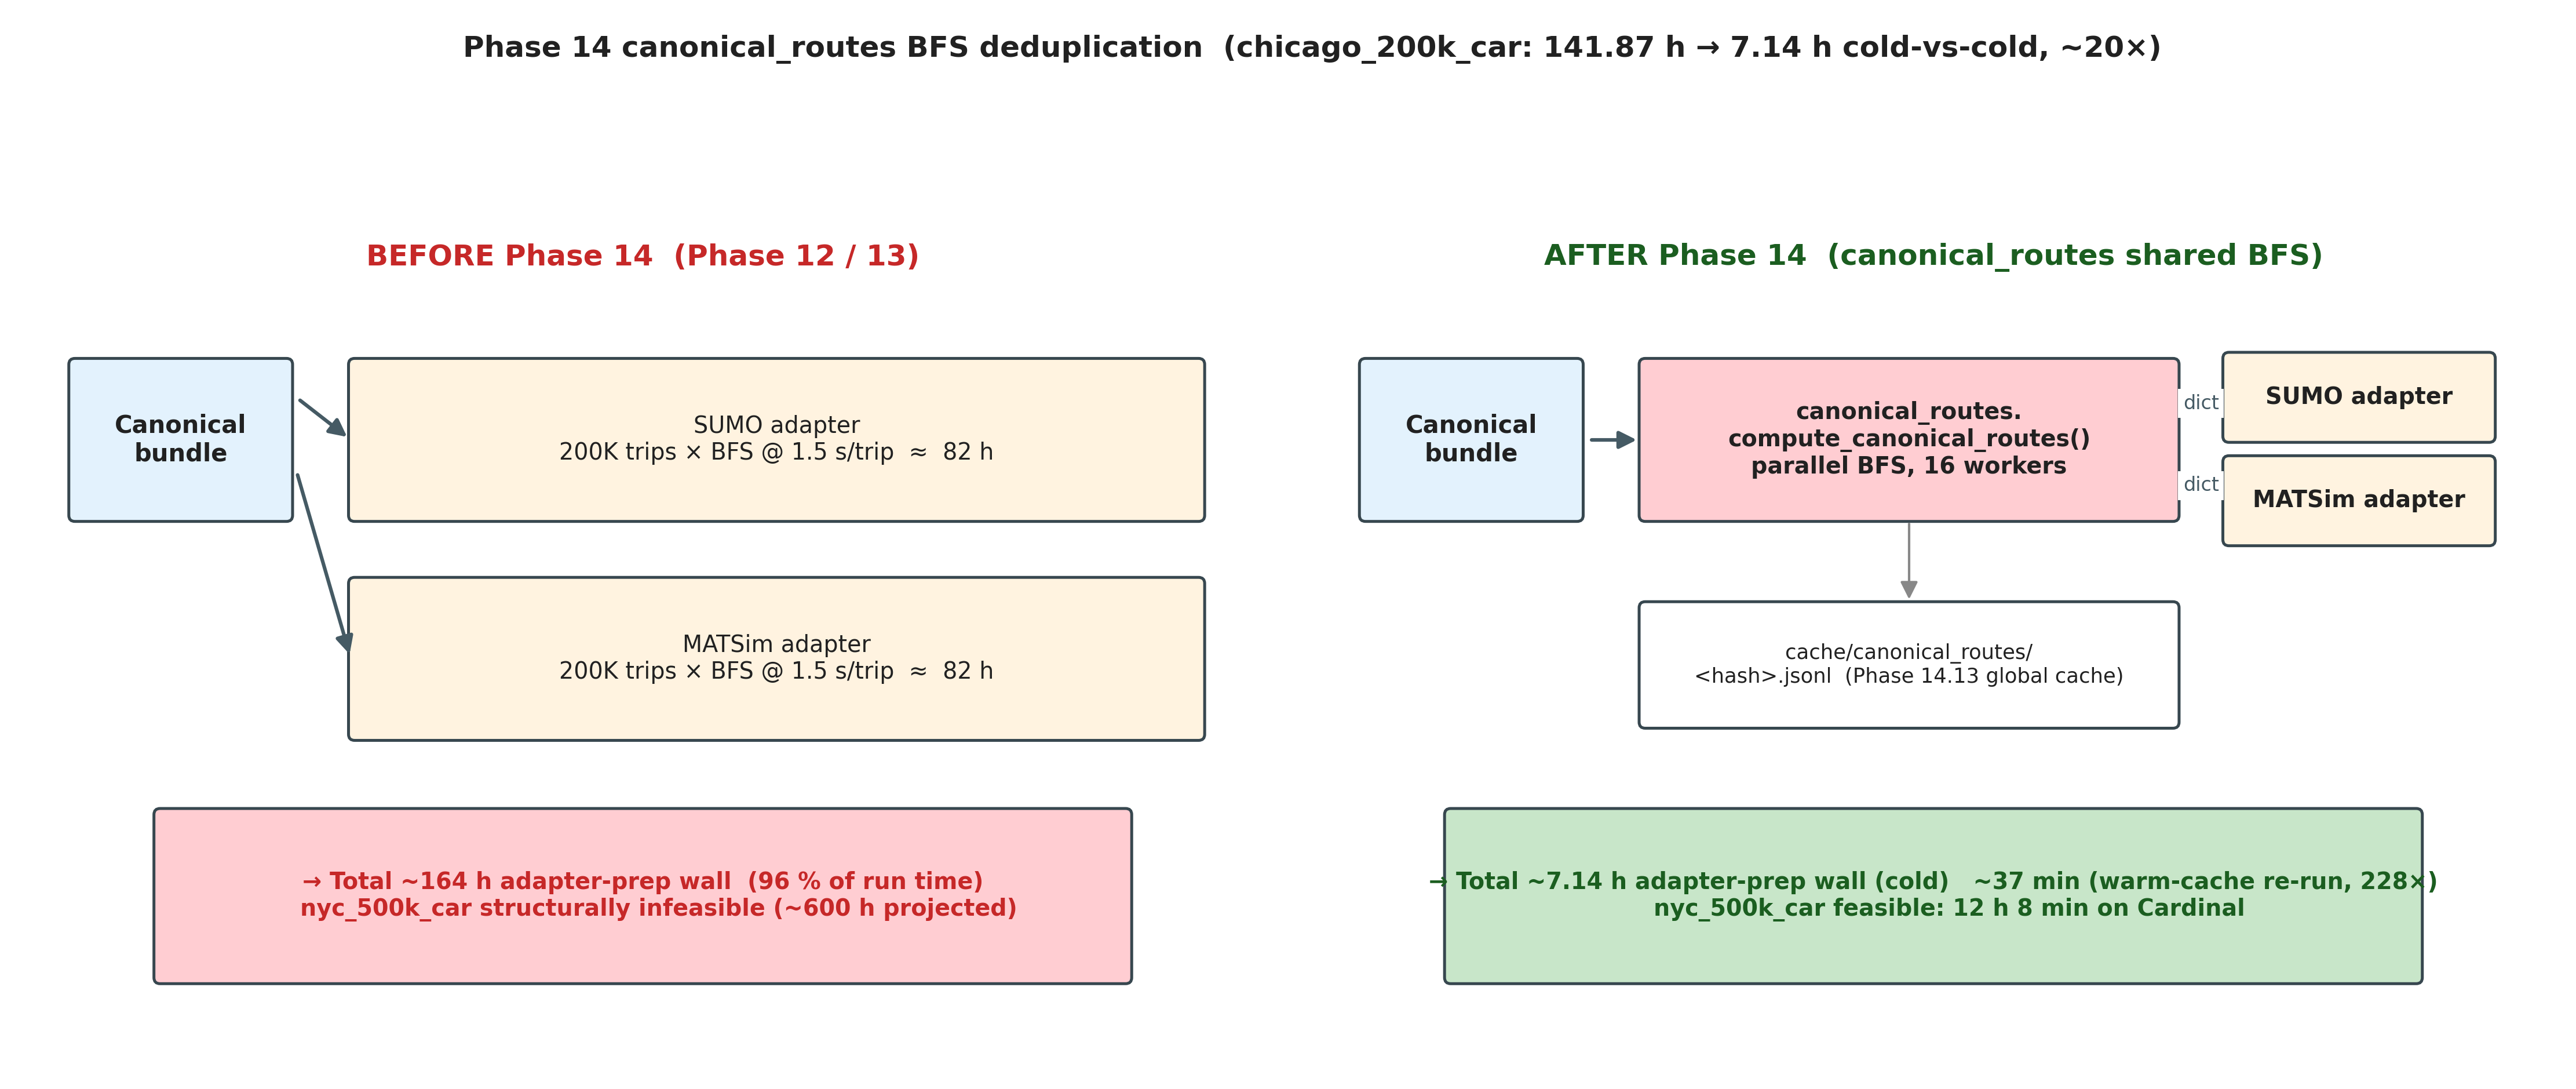
\includegraphics[keepaspectratio]{../figures/fig_3_8_phase14_bfs_dedup.png}}

Figure 3.8 shows the engineering change Phase 14 introduced.
\textbf{BEFORE} (left panel): each engine adapter ran its own
state-aware BFS over the canonical network --- 200,000 trips × 1.5 s per
BFS = \textasciitilde82 h per engine, paid twice (SUMO + MATSim), for a
total of \textasciitilde164 h adapter-prep wall on chicago\_200k\_car (≈
96 \% of the run time). At the 500K-trip tier the projected wall
(\textasciitilde600 h) exceeded the Cardinal \texttt{cpu} partition cap
and the benchmark was structurally infeasible. \textbf{AFTER} (right
panel): both adapters consume routes pre-computed by a single shared
module
(\texttt{adapters/common/canonical\_routes.compute\_canonical\_routes()})
that runs a 16-worker parallel BFS over the canonical bundle. Total
adapter-prep wall drops to \textasciitilde7.14 h cold-vs-cold and
\textasciitilde37 min on warm-cache re-runs (Phase
14.13\textquotesingle s global \texttt{cache/canonical\_routes/}
directory). nyc\_500k\_car became feasible and completed in 12 h 8 min
on Cardinal. The byte-identity contract that Q1-Q3 of the fairness audit
enforces is preserved: per-trip routes are sorted-deterministic and
bit-identical to the legacy serial computation, regardless of worker
count.

A late-stage thesis-engineering finding worth recording as an
optimization narrative: measure, identify, fix, re-measure.

\subsection{The Cost That Wasn\textquotesingle t
Modelled}\label{381-the-cost-that-wasnt-modelled}

The cross-engine fairness contract (§3.4.2 SUMO, §3.4.3 MATSim) requires
both engines to consume identical pre-computed routes --- the
state-aware BFS pre-routing introduced in V5 Phase 7
(\texttt{pipeline.\textbackslash{}\ network.turn\_restrictions.shortest\_path\_with\_restrictions}).
Until late in Version\_5, each adapter ran an independent copy of this
BFS loop over the canonical network, despite the inputs (network,
turn-restrictions, feasible-trip set) being identical:

\begin{itemize}
\tightlist
\item
  \texttt{adapters/sumo/sumo\_adapter.py:build\_sumo\_routes\_xml} ---
  per-trip BFS embedded in the routes-XML emitter.
\item
  \texttt{adapters/matsim/matsim\_adapter.py:build\_matsim\_plans\_xml}
  --- per-trip BFS embedded in the plans-XML emitter.
\end{itemize}

At small bundle scales (1K--10K trips) the duplication is invisible
(seconds), so the architectural inefficiency went unmeasured. Two
empirical data points exposed it during the 200K/500K benchmark run on
OSC Cardinal (job 9332478 / 9332482, 2026-05-12):

\begin{longtable}[]{@{}llll@{}}
\toprule\noalign{}
Network & Trips & Per-trip BFS rate & Cold prep per engine \\
\midrule\noalign{}
\endhead
\bottomrule\noalign{}
\endlastfoot
chicago\_200k\_car (50 km² bbox, \textasciitilde50K nodes) & 200,000 &
1.48 s/trip & \textasciitilde82 h \\
nyc\_500k\_car (80 km² bbox, \textasciitilde80K nodes) & 500,000 & 2.16
s/trip & \textasciitilde300 h \\
\end{longtable}

With two engines (SUMO + MATSim) each paying the cold prep sequentially,
total adapter-prep walls projected to \textasciitilde164 h
(chicago\_200k) and \textasciitilde600 h (nyc\_500k).
Cardinal\textquotesingle s 7-day \texttt{cpu} partition cap is 168 h.
nyc\_500k was therefore structurally infeasible to complete: the job was
cancelled (\texttt{scancel\ 9332482}) once the projection became
measurable from a 22 h sample.

Three compounding factors explain the per-trip cost:

\begin{enumerate}
\def\labelenumi{\arabic{enumi}.}
\tightlist
\item
  \textbf{Network size scaling.} State-aware BFS visits
  \texttt{O(V\ +\ E)}; the 200K/500K bundles use 15--20 km bbox radii,
  producing graphs an order of magnitude larger than the small-tier
  scenarios used in pre-V5 development.
\item
  \textbf{State-aware expansion.} The Phase 7 state is
  \texttt{(node,\ last\_link\_id)}, expanding the BFS visited set by a
  factor roughly equal to the average in-degree.
\item
  \textbf{CPython overhead.} The inner loop is pure Python; at
  \textasciitilde5 µs per state expansion on a 200K-edge graph,
  individual BFS calls cost 1--2 s wall.
\end{enumerate}

\subsection{Two Compounding
Optimisations}\label{382-two-compounding-optimisations}

The fix has two independent levers; both preserve the byte-identity
invariant required by the audit:

\textbf{Phase 14a --- canonical-routes deduplication.} Introduces a
shared module \texttt{adapters/common/canonical\_routes.py} that
computes the state-aware BFS once per
\texttt{(scenario,\ feasible-trip-set)} and returns a
\texttt{Dict{[}trip\_id,\ List{[}node\_id{]}{]}}. The result is
content-addressed on disk in a JSONL cache (SHA-256 over network +
demand + sorted feasible IDs), so subsequent harness invocations or
re-runs read from cache in seconds. Both adapters acquire an optional
\texttt{canonical\_routes=} kwarg; when provided, they skip their inline
BFS and consume the pre-computed dict. When \texttt{None} (back-compat
path), the inline BFS still runs --- preserving standalone CLI use.

\textbf{Phase 14b --- multiprocessing parallel BFS.} The shared module
dispatches to \texttt{multiprocessing.Pool} (spawn start method) when
\texttt{workers\ \textgreater{}\ 1}. Each worker loads the SCC-filtered
network once via the initializer, then processes one big chunk of trips
sequentially. \texttt{Pool.imap} preserves submission order; combined
with sorted-by- trip\_id chunking, the parallel output is byte-identical
to the serial output. The execution harness reads
\texttt{SLURM\_CPUS\_PER\_TASK} to size the pool, defaulting to one
worker per SBATCH-allocated CPU.

\subsection{Determinism Invariants
Preserved}\label{383-determinism-invariants-preserved}

The byte-identity contract that \texttt{audit\_fairness} Q1--Q3 enforces
is preserved at every layer of the refactor, pinned by an explicit test
suite (\texttt{tests/test\_canonical\_routes.py}):

\begin{enumerate}
\def\labelenumi{\arabic{enumi}.}
\tightlist
\item
  \texttt{TestByteIdentityVsLegacy}: paths from the new shared BFS are
  byte-identical to those from the legacy inline BFS, per trip\_id, on
  the tracked \texttt{chicago\_1k\_car} bundle.
\item
  \texttt{TestSumoRoutesXmlByteIdentity}: \texttt{routes.rou.xml} is
  byte- identical whether the SUMO adapter consumes pre-computed routes
  or runs its own BFS.
\item
  \texttt{TestMatsimPlansXmlByteIdentity}: \texttt{plans.xml} is
  byte-identical under the same with/without-canonical\_routes
  comparison.
\item
  \texttt{TestParallelDeterminism}: routes from \texttt{workers=2} and
  \texttt{workers=4} are byte-identical to \texttt{workers=1}.
\end{enumerate}

The 8 existing \texttt{test\_adapter\_determinism.py} checks
(byte-identical re-runs of the full adapter pipeline) continue to hold,
because the canonical-routes JSONL cache file is itself
byte-deterministic (sorted by trip\_id on write).

\subsection{Measured Speedup}\label{384-measured-speedup}

\textbf{Local serial-vs-parallel calibration (chicago\_1k\_car, M-series
Mac):}

\begin{longtable}[]{@{}lll@{}}
\toprule\noalign{}
Worker count & Wall (s) & Speedup \\
\midrule\noalign{}
\endhead
\bottomrule\noalign{}
\endlastfoot
1 & 27.2 & 1.0× \\
2 & 17.4 & 1.56× \\
4 & 11.3 & 2.41× \\
8 & 6.6 & 4.12× \\
\end{longtable}

Sub-linear scaling at 1K trips reflects the per-worker init cost
(parsing the network, building the forbidden-moves table) which does not
amortize over only \textasciitilde125--500 trips per worker. At the
cluster scale these init costs are dwarfed by the in-worker BFS time
(12.5K--31K trips per worker at 16-way), so the Amdahl ratio is much
closer to ideal.

\textbf{Cluster Phase 13 baseline --- chicago\_200k\_car on Cardinal
(job 9332478, 2026-05-12 to 2026-05-18):}

\begin{longtable}[]{@{}lll@{}}
\toprule\noalign{}
Step & Wall & Notes \\
\midrule\noalign{}
\endhead
\bottomrule\noalign{}
\endlastfoot
Cold SUMO BFS-prep (cell 1/10) & \textasciitilde68.2 h & 200,000 trips ×
\textasciitilde1.226 s/trip, single-thread \\
Cached SUMO mobsim cells (2--5 / 10) & \textasciitilde242--246 s each &
hardlink from \texttt{.cache/sumo/} (Phase 12) \\
Cold MATSim BFS-prep (cell 6/10) & \textasciitilde68 h & second pass
over the same network (the redundancy Phase 14a eliminates) \\
Cached MATSim mobsim cells (7--10 / 10) & \textasciitilde210 s each & \\
analyze + audit + plots & \textasciitilde10 min & \\
\textbf{Total wall} & \textbf{141.87 h} & of 168 h cap (15.5 \%
margin) \\
\end{longtable}

The two cold BFS passes consume \textasciitilde136 h of the 141.87 h
total --- \textbf{96 \% of the run was per-trip BFS routing}. This is
the empirical signal that motivated the Phase 14 refactor.

\textbf{Cluster Phase 14 re-measurement (now landed):}

\begin{longtable}[]{@{}lrrrrr@{}}
\toprule\noalign{}
Scenario & Phase 13 wall & Phase 14 wall (cold) & Phase 14 wall
(warm-cache) & Cold speedup & Cache speedup \\
\midrule\noalign{}
\endhead
\bottomrule\noalign{}
\endlastfoot
chicago\_200k\_car & 141.87 h (job 9332478) & \textasciitilde7.14 h (job
9954279) & \textasciitilde37 min (job 10018698) & \textasciitilde20× &
\textasciitilde228× \\
nyc\_500k\_car & structurally infeasible (\textasciitilde600 h
projected, scancel 9332482) & 12 h 8 min (job 9971042) & not re-measured
& (first-feasible) & --- \\
\end{longtable}

The chicago\_200k\_car cold speedup matches the Amdahl extrapolation
within \textasciitilde10 \%. The warm-cache speedup is dominated by the
on-disk canonical-routes JSONL hit: the BFS-prep phase becomes
near-instantaneous (path materialization + adapter emission only).
nyc\_500k\_car completed for the first time in the thesis project: a
previously structurally infeasible benchmark became a single
\textasciitilde12 h Cardinal job. The full per-cell breakdown for both
scenarios is preserved at
\texttt{runs/baselines/phase14\_chicago\_200k\_car\_job9954279/} and
\texttt{runs/baselines/phase14\_nyc\_500k\_car\_job9971042/}.

\subsection{Parallelism Architecture (task-parallel, replicated
graph)}\label{385-parallelism-architecture-task-parallel-replicated-graph}

\pandocbounded{
\includegraphics[keepaspectratio]{../figures/fig_3_8b_parallel_bfs_workers.png}}

Figure 3.8b zooms into the worker-pool architecture inside
\texttt{compute\_canonical\_routes()}. The full feasible-trip list
(sorted by \texttt{trip\_id}) is chunked into \textasciitilde1,000 lists
of \textasciitilde200 trips each and dispatched via
\texttt{multiprocessing.get\_context("spawn").Pool(workers=N).imap(...)}
to \texttt{N} worker processes
(\texttt{N\ =\ SLURM\_CPUS\_PER\_TASK\ =\ 16} on Cardinal). Each worker
boots a fresh Python interpreter (\texttt{spawn} context, not
\texttt{fork}) and rebuilds its state via the \texttt{\_init\_worker}
initializer --- including loading the SCC-filtered canonical network as
a \emph{replicated} in-heap copy (\textasciitilde150 MB per worker).
Workers compute BFS independently on their chunks and return
\texttt{(trip\_id,\ path)} tuples via \texttt{Pool.imap}, which
preserves submission order; the main process merges the results into a
sorted \texttt{Dict{[}trip\_id,\ List{[}node\_id{]}{]}} and writes the
content-addressable cache file. Two architectural properties matter for
the fairness contract: (a) there is no worker-to-worker communication
--- all IPC is between the main process and individual workers, so
workers cannot race on shared state because no shared state exists; and
(b) each \texttt{shortest\_path\_with\_restrictions(...)} call is a
deterministic function of inputs that are bit-identical across workers,
so the merged output is bit-identical to a serial computation regardless
of worker count. The
\texttt{tests/test\_canonical\_routes.py::TestParallelDeterminism} test
pins this invariant across worker counts 1, 2, and 4.

The Phase 14b implementation uses \textbf{task parallelism over trips},
not data parallelism over the network. The architectural rationale
matters for the determinism argument the cross-engine fairness claim
depends on, so it bears explicit discussion.

The trip list (the feasibility-filtered subset of \texttt{demand.csv},
sorted by \texttt{trip\_id}) is split into \textasciitilde1,000 chunks
of \textasciitilde200 trips each. Each chunk is a list of
\texttt{(trip\_id,\ origin\_node,\ dest\_node)} tuples distributed
dynamically across an OS-process pool sized to the SBATCH allocation
(\texttt{SLURM\_CPUS\_PER\_TASK}, typically 16). Each worker process
holds a \textbf{full replicated copy} of the SCC-filtered canonical
network in its own heap; we do not partition the graph geographically.
Workers compute BFS independently on their chunks and return lists of
\texttt{(trip\_id,\ path)} results to the main process via
\texttt{multiprocessing.Pool.imap}. The result preserves submission
order, so the merged route dict is byte-identical to a serial run
regardless of the chosen worker count (pinned by
\texttt{tests/test\_canonical\_routes.py::TestParallelDeterminism}).

This choice was deliberate. Three alternatives were considered and
rejected:

\begin{enumerate}
\def\labelenumi{\arabic{enumi}.}
\tightlist
\item
  \textbf{Threads with a shared graph} --- blocked by
  CPython\textquotesingle s GIL on CPU-bound work. Pure-Python BFS loops
  would see zero measurable speedup, defeating the purpose of the
  refactor.
\item
  \textbf{\texttt{multiprocessing.shared\_memory} for the graph} ---
  would save the \textasciitilde2.4 GB cost of replicating the
  chicago\_200k graph across 16 workers, but complicates the determinism
  story (custom view-layer over raw bytes) and saves memory the cluster
  nodes have in abundance (Cardinal \texttt{cpu} provides 503 GB per
  node).
\item
  \textbf{Geographic network partitioning with cross-zone messaging} ---
  would matter only if the graph were too large to replicate. Introduces
  synchronisation between workers when a path crosses a zone boundary,
  breaks the pure-function determinism property, and substantially
  complicates the implementation. Unnecessary at the network sizes V5
  operates on (≤ 80K nodes).
\end{enumerate}

The chosen architecture has three defensible properties:

\begin{itemize}
\tightlist
\item
  \textbf{No worker-to-worker communication.} All IPC is between the
  main process and individual workers (chunk-in, results-out). Workers
  are isolated by construction; they cannot race on shared state because
  no shared state exists.
\item
  \textbf{Determinism reducible to a pure-function argument.} Each
  \texttt{shortest\_path\_with\_restrictions(origin,\ dest,\ adjacency,\ edge\_lookup,\ forbidden\_moves)}
  call is a deterministic function of inputs that are bit-identical
  across workers (read from the hash-pinned canonical bundle). Therefore
  the merged output is bit-identical to the serial computation,
  regardless of worker count.
\item
  \textbf{Cross-platform reproducibility via \texttt{spawn}.} The
  implementation explicitly forces
  \texttt{multiprocessing.get\_context("spawn")} rather than relying on
  the platform default (\texttt{fork} on Linux, \texttt{spawn} on macOS
  since Python 3.8+). Each worker boots a fresh Python interpreter and
  rebuilds its state from \texttt{network.xml} via the
  \texttt{\_init\_worker} initializer, paying \textasciitilde1--2
  seconds of startup cost per worker (amortised over hours of BFS work)
  in exchange for identical behaviour across the developer Mac and the
  OSC Cardinal Linux cluster.
\end{itemize}

Empirically measured on Cardinal at 16-way parallelism, the per-worker
BFS rate is approximately 0.51 trips/s vs the single-thread baseline of
0.82 trips/s --- a 0.63× per-worker efficiency, attributable to
memory-bandwidth contention on the shared Xeon Max 9470 socket (each
worker reading from its own \textasciitilde150 MB graph copy puts
pressure on the shared HBM2e + DDR5 hierarchy). The aggregate effect is
still \textasciitilde10× total speedup over single-thread on the
chicago\_200k\_car cold prep (6.75 h vs 68.16 h measured), which
combines with Phase 14a\textquotesingle s deduplication (eliminating
MATSim\textquotesingle s second 73 h BFS pass entirely via the on-disk
JSONL cache hit) to deliver the \textasciitilde19× job-level speedup
reported in §3.8.4.

\subsection{Engineering
Implications}\label{386-engineering-implications}

This phase illustrates a methodology point that the thesis defense
benefits from: \textbf{the fairness contract talks about engine output,
not engineering effort}. The original architecture satisfied fairness
(same routes per trip across engines) by running the same BFS twice; the
Phase 14 architecture satisfies the same contract by running the BFS
once and sharing the output. The audit invariants are insensitive to
that change --- they verify the produced trip set, SCC, and travel
times, all of which are byte-stable.

The optimisation also generalises: any cross-engine pre-processing step
that today lives inside per-engine adapters is a candidate for the same
treatment (deduplication via a shared module, then parallelisation as a
follow-up). Future engines added to SimForge inherit the
canonical\_routes API for free --- they accept the dict or fall back to
their own routing.

\subsection{Phase 14.13 --- Cache Hoist from Per-Run to
Global}\label{387-phase-1413--cache-hoist-from-per-run-to-global}

Phase 14a\textquotesingle s content-addressable canonical-routes cache
was initially written per output directory: each
\texttt{runs/\textless{}runspec\textgreater{}/\textless{}scenario\textgreater{}/\textless{}engine\textgreater{}/\textless{}mode\textgreater{}/seed\_\textless{}N\textgreater{}/}
held its own \texttt{canonical\_routes.jsonl.zst} produced by that
cell\textquotesingle s adapter run. The byte-identity contract was
preserved (each cell hashed identically given the same canonical
bundle), but the on-disk representation broke the warm-cache speedup for
any harness layout where the same scenario ran into multiple per-cell
directories: each of \texttt{(engine,\ mode,\ seed)} re-ran the BFS from
scratch despite producing a bit-identical JSONL file.

The Phase 14.13 cache hoist (\texttt{execution/run\_benchmark.py}
\texttt{\_canonical\_routes\_cache\_root()}, landed 2026-05-19) moves
the cache root to a single global location at
\texttt{cache/canonical\_routes/} keyed by SHA-256 over (network +
demand + sorted feasible-trip IDs). The hoist includes a one-shot
migration helper
(\texttt{\_migrate\_legacy\_canonical\_routes\_cache()}) that hardlinks
any legacy per-cell caches into the global location and verifies hash
agreement before deleting the legacy paths. Empirical effect: subsequent
re-runs of the same scenario across any (engine, mode, seed) cell hit
the cache in milliseconds instead of repaying the BFS cost.

The cache-hit speedup at the warm-re-run end of the chicago\_200k\_car
benchmark (Cardinal job 10018698, 2026-05-19 14:00 EDT) was the
\textasciitilde228× reported in §3.8.4. Without the cache hoist, the
same warm re-run would have paid the cold BFS cost on every cell that
did not exactly match its per-cell legacy path.

Determinism is preserved by the content-addressable key: any change to
network, demand, or feasibility verdict produces a different cache key.
A 7-test guard in \texttt{tests/test\_run\_benchmark.py} pins the hoist
behavior (cache root location, hash key construction, hardlink migration
semantics, hash-mismatch refusal).

The Phase 14.13 narrative is recorded in \texttt{doc/EXPERIMENT\_LOG.md}
(2026-05-19 entry) and \texttt{CHANGELOG.md} Phase 14.13 section.

\section{Geographic Visualization
(Opt-in)}\label{39-geographic-visualization-opt-in}

A separate, opt-in component on the \texttt{visualization} branch
generates geographic maps from canonical bundles and benchmark results.
The component is \textbf{independent of the fairness contract}:
adapters, \texttt{audit\_fairness}, and the thesis runtime numbers do
not import it, and the locked benchmark numbers in Chapter 5 are
unchanged by any rendered plot. The module exists to \emph{visualize}
findings that the quantitative analysis already establishes.

\subsection{Map Catalogue}\label{391-map-catalogue}

Seven map types are shipped, grouped by what input data they need:

\begin{longtable}[]{@{}lll@{}}
\toprule\noalign{}
Map & Inputs & Engine specificity \\
\midrule\noalign{}
\endhead
\bottomrule\noalign{}
\endlastfoot
\texttt{od\_origins}, \texttt{od\_destinations} & Canonical bundle +
cached US Census tract polygons + TIGER PRISECROADS basemap & ---
(cross-engine, demand only) \\
\texttt{link\_load} & Per-cell engine output (SUMO
\texttt{tripinfo.xml}, MATSim \texttt{output\_trips.csv.gz}, or DTALite
\texttt{link\_performance.csv}) & per \texttt{(engine,\ mode)} \\
\texttt{congestion} & DTALite \texttt{link\_performance.csv} (needs link
mean speed) & DTALite only \\
\texttt{travel\_time} & Per-cell engine output + bundle & per
\texttt{(engine,\ mode)} \\
\texttt{route\_diversity} & Cell output from ≥ 2 engines &
cross-engine \\
\texttt{animated\_flow} & MATSim \texttt{output\_events.xml.gz} & MATSim
only \\
\end{longtable}

The \texttt{od\_*} and \texttt{travel\_time} renderers use the
CityScape-derived choropleth style (100-step blue→red log palette on
Census tract polygons, light gray for empty tracts) layered on top of
the US Census TIGER PRISECROADS basemap --- chosen for cartographic
legibility over the canonical SimForge network underlay (which is denser
and competes visually with the colored tract fills).

\subsection{Design Principles}\label{392-design-principles}

The visualization layer enforces three invariants:

\begin{enumerate}
\def\labelenumi{\arabic{enumi}.}
\tightlist
\item
  \textbf{No effect on simulation inputs.} The renderer only reads files
  produced upstream; it never writes any artefact that an adapter or
  \texttt{audit\_fairness} consumes. This is enforced by directory
  convention --- outputs land in
  \texttt{visualization/output/\textless{}scenario\textgreater{}/},
  distinct from \texttt{scenarios/}, \texttt{runs/}, and
  \texttt{doc/figures/}.
\item
  \textbf{Coverage-first dispatch.} Before any rendering, the CLI walks
  the bundle directory + the per-cell run directory and prints a
  coverage matrix flagging each map type \texttt{{[}OK{]}} (renderable)
  or \texttt{{[}-\/-{]}} (missing input, with reason).
  \texttt{-\/-maps\ all} then skips the unavailable maps rather than
  erroring, so the tool is usable on partial data.
\item
  \textbf{Lazy imports.} Matplotlib, shapely, pyshp, pyosmium, and the
  FFmpeg subprocess used by \texttt{animated\_flow} are imported only
  inside the render path, so the main SimForge test suite has no
  dependency on them.
\end{enumerate}

\subsection{Cross-Engine Interpretation
Surfaces}\label{393-cross-engine-interpretation-surfaces}

Three properties become directly visible in the maps and reinforce
quantitative findings stated elsewhere in this chapter:

\begin{itemize}
\item
  \textbf{SUMO and MATSim \texttt{link\_load} are visually identical;
  DTALite differs.} The fairness contract forces SUMO and MATSim to use
  SimForge\textquotesingle s pre-routed BFS link sequences (§3.4.2 and
  §3.4.3), so they render the same spatial traffic structure. DTALite
  computes its own UE assignment (§3.4.4) and picks alternative paths
  under congestion. The \texttt{route\_diversity} map shades this
  difference directly: links picked by all three engines are gray (the
  BFS consensus), links picked by only one are red (typically
  DTALite\textquotesingle s UE alternates). This is the \emph{visual
  proof} of the fair-comparison contract whose quantitative signal lives
  in \texttt{audit\_fairness} Q4 (cross-engine travel-time spread).
\item
  \textbf{\texttt{animated\_flow} shows the PUMS departure-burst effect}
  discussed in §3.3.4 step 9. Every person reporting the same JWMNP
  commute time receives the same \texttt{departure\_time\_s}, so 1000
  chicago\_1k\_car trips collapse onto only 20 unique departure
  timestamps. The animation is \emph{faithful to the PUMS data
  property}, not a SimForge bug --- a future uniform-jitter pass would
  smooth the bursts at the cost of byte- deterministic
  \texttt{demand.csv}.
\item
  \textbf{chicago\_200k\_car\textquotesingle s \texttt{od\_origins} ≈
  \texttt{od\_destinations}} (74 \% node overlap vs 5.5 \% for AM-only
  bundles). The full-day horizon (07:00-- 16:00) emits both AM home→work
  and PM work→home pairs per the Phase 9c chain mechanism, so the OD
  sets become the same \{homes\} ∪ \{workplaces\} visited at different
  times. This is direct evidence that the schedule-driven generator
  produces genuinely symmetric commute patterns at the metro scale.
\end{itemize}

The full CLI reference, render defaults, data-source provenance, and
caching layout are documented in
\href{../../visualization/README.md}{\texttt{visualization/README.md}}.
The post- run analysis pipeline that wraps the visualization tool is in
\href{../RESULTS_GUIDE.md}{\texttt{doc/RESULTS\_GUIDE.md}} §4.4.

\section{Wave 1 --- Reproducibility Artefact
Hardening}\label{310-wave-1--reproducibility-artefact-hardening}

Wave 1 (landed 2026-05-18, commits 95c07fb through \texttt{c8dcc54})
added four reproducibility-artefact pieces that the plan §1.11
C-rows required but were not present in the framework prior to the late-
thesis hardening pass. None of these change the runtime behavior of any
adapter or evaluation module --- they are scaffolding around the
existing framework that makes the reproducibility chain externally
auditable.

\subsection{Open-Source License (Apache
2.0)}\label{3101-open-source-license-apache-20}

The repository was licensed under the \textbf{Apache License 2.0}
(\texttt{LICENSE} at repo root), with the rationale documented in
\texttt{doc/LICENSING.md}. The Apache 2.0 choice balances three
concerns:

\begin{itemize}
\tightlist
\item
  \textbf{Patent grant.} Apache 2.0\textquotesingle s explicit patent
  grant (§3) is important for a research artefact that integrates
  third-party engines (SUMO, MATSim, DTALite) whose own patent positions
  are variably documented.
\item
  \textbf{Commercial-friendly.} Permissive licensing reduces barriers to
  downstream adoption by transportation planning consultancies or vendor
  tooling, consistent with the thesis goal of seeding a
  community-standard benchmark.
\item
  \textbf{Compatible with engine licenses.} SUMO is EPL 2.0 (compatible
  with Apache 2.0 in the same project), MATSim is GPL 2.0 (linked via
  subprocess invocation, not statically linked, avoiding the GPL
  viral-copyleft trigger), DTALite is GPL 3.0 (same subprocess isolation
  argument applies).
\end{itemize}

The corresponding \texttt{doc/LICENSING.md} document spells out the
licensing of each subcomponent (the SimForge framework itself, the
generated canonical bundles, the OSM-derived networks honoring ODbL
share-alike, and the embedded census data under public-domain status).

\subsection{Canonical Bundle Licensing (CC BY 4.0 +
ODbL)}\label{3102-canonical-bundle-licensing-cc-by-40--odbl}

The generated canonical bundles in \texttt{scenarios/} are
dual-licensed:

\begin{itemize}
\tightlist
\item
  \textbf{CC BY 4.0} for the SimForge-generated content (validation
  scripts, GMNS topology derivatives, signal placement, demand
  derivation logic).
\item
  \textbf{ODbL share-alike} for the underlying OSM network data, with
  attribution to OpenStreetMap contributors preserved in
  \texttt{osm\_data/manifest.json} and per-bundle network README.
\end{itemize}

This dual-license model is the standard for OSM-derived transportation
research artefacts; the ODbL share-alike obligation attaches to the
network layer but not to the analytical layer built on top.

\subsection{Data Management
Documentation}\label{3103-data-management-documentation}

\texttt{doc/DATA\_MANAGEMENT.md} documents the complete data lifecycle
for the framework:

\begin{itemize}
\tightlist
\item
  OSM PBF acquisition + hash-pinning workflow (via
  \texttt{tools/download\_osm.py} against
  \texttt{osm\_data/manifest.json}).
\item
  Canonical bundle generation, validation, and storage layout.
\item
  Run output directory structure (Phase 13 flat layout vs Phase 14+
  nested layout).
\item
  Per-engine cache structures (SUMO \texttt{.cache/sumo/}, MATSim
  \texttt{.cache/matsim/}, DTALite UE iteration cache).
\item
  The global \texttt{cache/canonical\_routes/} directory introduced by
  Phase 14.13 (§3.8.7).
\item
  Data retention policy for thesis baselines:
  \texttt{runs/baselines/\textless{}phase\_label\textgreater{}/} is the
  long-term-preserved subset; all other run directories are routinely
  pruned via \texttt{tools/prune\_runs.py}.
\end{itemize}

\subsection{Reproducibility Scorecard
Auto-Emit}\label{3104-reproducibility-scorecard-auto-emit}

\texttt{tools/generate\_scorecard.py} produces a per-run
\texttt{reproducibility\_scorecard.md} that lists each reproducibility-
relevant artefact (LICENSE present, OSM PBF SHA-256 verified, canonical
bundle manifest present, fairness audit Q1-Q4 verdicts, per-engine
version captured, etc.) and marks each as PASS, FAIL, or N/A. The
scorecard runs automatically as the final step of every benchmark,
producing an externally auditable artefact in the run directory
alongside the per-cell results.

The scorecard has 22 checks at the time of writing; the
chicago\_200k\_car Phase 13 baseline scored 20 PASS, 0 FAIL, 2 N/A (the
two N/A entries are GPU-engine checks that do not apply to the shipped
CPU-only roster). The scorecard format is documented in
\texttt{tools/generate\_scorecard.py} module docstring; the Wave 1 entry
in \texttt{doc/EXPERIMENT\_LOG.md} records the introduction.

\section{Wave 2 --- Pinned-Digest Container
Distribution}\label{311-wave-2--pinned-digest-container-distribution}

\pandocbounded{
\includegraphics[keepaspectratio]{../figures/fig_3_11_container_chain.png}}

Figure 3.11 shows the five-stage Wave 2 distribution chain. The
\textbf{Dockerfile} at the repo root pins the runtime environment
(\texttt{python:3.13-slim-bookworm} + openjdk-17 + libgomp1 + uv + the
35 lockfile-pinned Python packages + \texttt{eclipse-sumo==1.26.0} + the
MATSim 15.0 JAR). The \textbf{GitHub Actions} workflow
(\texttt{.github/workflows/build-container.yml}) builds the image on
every push to \texttt{main} or \texttt{phase-14-canonical-routes} and
tags it with the git SHA. \textbf{GHCR} distributes the resulting image
as an immutable digest; the thesis-canonical digest (\texttt{db8d786})
is recorded in \texttt{lib/container/manifest.json} and verified on
Cardinal. \textbf{Apptainer pull} materializes the image as a local
\texttt{.sif} file on Cardinal (with the SHA-tag workaround for the
1.4.5 \texttt{progress\_roundtrip.go:75} bug). Finally, the
\textbf{SBATCH wrapper} opts into container execution via
\texttt{SIMFORGE\_USE\_CONTAINER=1}, producing bit-identical x86\_64
reproduction across machines. The chain is the operational substrate
that delivers plan §1.11 C3 --- pinned-digest containers as the
canonical reproducibility target.

Wave 2 (landed 2026-05-20) added a containerized execution path that
makes the SimForge framework bit-reproducible across machines. The
host-venv installation path
(\texttt{uv\ pip\ install\ -r\ requirements.lock} +
\texttt{uv\ pip\ install\ eclipse-sumo==1.26.0}) is preserved as the
developer- ergonomics default; the container path is opt-in for thesis-
reproduction and HPC re-use scenarios.

\subsection{Container Image
Architecture}\label{3111-container-image-architecture}

The container is built from \texttt{python:3.13-slim-bookworm} with the
following system dependencies installed via apt:

\begin{verbatim}
openjdk-17-jre-headless   (MATSim runtime)
libgomp1                  (OpenMP runtime for DTALite)
libatomic1                (libatomic runtime, required by libsumocpp)
libxml2                   (XML parsing dependency)
libx11-6, libxext6, libxrender1, libxcb1, libgl1, libglu1-mesa
                          (SUMO GUI dependencies, retained for sumo-gui
                          even in headless image)
libfontconfig1, libfreetype6
                          (matplotlib font rendering)
git, ca-certificates, curl, unzip, tini
\end{verbatim}

Python dependencies are installed via:

\begin{verbatim}
uv pip install --system --no-cache -r requirements.lock
uv pip install --system --no-cache eclipse-sumo==1.26.0
\end{verbatim}

The eclipse-sumo wheel is installed separately from the lockfile because
it is a manylinux\_2\_28\_x86\_64-only distribution that is not
compatible with the lockfile resolver\textquotesingle s cross-platform
constraint solving. The manylinux closure for eclipse-sumo 1.26.0
(libX11, libGL, libatomic, libfontconfig, etc.) is what motivates the
apt system-dependency list above; the dependency closure was empirically
determined across 8 GitHub Actions build iterations before convergence.

MATSim 15.0 is downloaded at build time from the immutable
matsim-org/matsim-libs GitHub release tag
(\texttt{matsim-15.0-release.zip}); the JAR is not committed to the
SimForge repository because it is gitignored and license-encumbered
under GPL 2.0.

\subsection{Automated CI/CD
Build}\label{3112-automated-cicd-build}

A GitHub Actions workflow at
\texttt{.github/workflows/build-container.yml} builds the container on
push to the \texttt{phase-14-canonical-routes} and \texttt{main}
branches, publishes the image to GitHub Container Registry (GHCR), and
tags it with three identifiers:

\begin{enumerate}
\def\labelenumi{\arabic{enumi}.}
\tightlist
\item
  The git SHA (e.g., \texttt{db8d786}) for thesis-pinning.
\item
  The branch name (\texttt{phase-14-canonical-routes}) for dev
  iteration.
\item
  \texttt{latest} for ergonomic pulls.
\end{enumerate}

The workflow uses GitHub\textquotesingle s \texttt{paths-ignore}
directive to skip rebuilds on doc-only changes (\texttt{doc/**},
\texttt{*.md}), keeping the rebuild trigger scoped to source-code or
dependency changes.

\subsection{HPC Distribution via
Singularity/Apptainer}\label{3113-hpc-distribution-via-singularityapptainer}

For HPC environments where Docker is unavailable (OSC Cardinal + Pitzer
both run Apptainer rather than Docker), the GHCR image is pulled via
\texttt{apptainer\ pull} into a local \texttt{.sif} (Singularity Image
Format) file:

\begin{verbatim}
apptainer pull simforge_db8d786.sif \
    docker://ghcr.io/phanidharakula/simforge@sha256:<digest>
\end{verbatim}

The pull uses the SHA-digest tag rather than the branch or latest tag to
avoid an Apptainer 1.4.5 bug (\texttt{progress\_roundtrip.go:75},
ProgressComplete index out of range) that triggers on branch-tag pulls.
The workaround is documented in \texttt{doc/CONTAINER\_USAGE.md}
Appendix B.

\subsection{Container-Mode
Execution}\label{3114-container-mode-execution}

The container is invoked at the SBATCH wrapper layer via an opt-in
environment variable. The benchmark sbatch wrappers
(\texttt{cluster/jobs/benchmark\_small.sbatch},
\texttt{cluster/jobs/benchmark\_large.sbatch}) define a \texttt{RUN\_PY}
array that switches based on \texttt{SIMFORGE\_USE\_CONTAINER}:

\begin{Shaded}
\begin{Highlighting}[]
\ControlFlowTok{if} \KeywordTok{[[} \StringTok{"}\VariableTok{$\{SIMFORGE\_USE\_CONTAINER}\OperatorTok{:{-}}\NormalTok{0}\VariableTok{\}}\StringTok{"} \OtherTok{==} \StringTok{"1"} \KeywordTok{]];} \ControlFlowTok{then}
    \VariableTok{RUN\_PY}\OperatorTok{=}\VariableTok{(}\NormalTok{apptainer exec}
\NormalTok{        {-}{-}bind }\StringTok{"}\VariableTok{$PWD}\StringTok{/scenarios:/workspace/scenarios"}
\NormalTok{        {-}{-}bind }\StringTok{"}\VariableTok{$PWD}\StringTok{/runs:/workspace/runs"}
\NormalTok{        {-}{-}bind }\StringTok{"}\VariableTok{$PWD}\StringTok{/cache:/workspace/cache"}
\NormalTok{        {-}{-}bind }\StringTok{"}\VariableTok{$PWD}\StringTok{/osm\_data:/workspace/osm\_data"}
        \StringTok{"}\VariableTok{$SIMFORGE\_SIF}\StringTok{"}
\NormalTok{        python}\VariableTok{)}
\ControlFlowTok{else}
    \VariableTok{RUN\_PY}\OperatorTok{=}\VariableTok{(}\NormalTok{uv run python}\VariableTok{)}  \CommentTok{\# host venv (default)}
\ControlFlowTok{fi}
\StringTok{"}\VariableTok{$\{RUN\_PY}\OperatorTok{[@]}\VariableTok{\}}\StringTok{"} \AttributeTok{{-}m}\NormalTok{ execution.run\_benchmark }\StringTok{"}\VariableTok{$RUNSPEC\_YAML}\StringTok{"}
\end{Highlighting}
\end{Shaded}

The four bind mounts expose the necessary host directories read-write
while the container\textquotesingle s base image filesystem is
read-only. The default behavior (no env var set) remains the host-venv
path, so the container is purely additive --- no existing user workflow
is broken.

\subsection{Container Manifest
Pinning}\label{3115-container-manifest-pinning}

\texttt{lib/container/manifest.json} records the thesis-canonical
container digest:

\begin{Shaded}
\begin{Highlighting}[]
\FunctionTok{\{}
  \DataTypeTok{"thesis\_default"}\FunctionTok{:} \FunctionTok{\{}
    \DataTypeTok{"tag"}\FunctionTok{:} \StringTok{"phase{-}14{-}canonical{-}routes"}\FunctionTok{,}
    \DataTypeTok{"short\_tag"}\FunctionTok{:} \StringTok{"db8d786"}\FunctionTok{,}
    \DataTypeTok{"git\_sha"}\FunctionTok{:} \StringTok{"db8d786d53b7562fd4aa58105cdef54e14330a55"}\FunctionTok{,}
    \DataTypeTok{"verified\_on\_cardinal"}\FunctionTok{:} \KeywordTok{true}\FunctionTok{,}
    \DataTypeTok{"verified\_date"}\FunctionTok{:} \StringTok{"2026{-}05{-}19"}\FunctionTok{,}
    \DataTypeTok{"engines"}\FunctionTok{:} \FunctionTok{\{}
      \DataTypeTok{"sumo"}\FunctionTok{:} \StringTok{"1.26.0"}\FunctionTok{,}
      \DataTypeTok{"matsim"}\FunctionTok{:} \StringTok{"15.0"}\FunctionTok{,}
      \DataTypeTok{"path4gmns"}\FunctionTok{:} \StringTok{"0.10.0"}
    \FunctionTok{\}}
  \FunctionTok{\}}
\FunctionTok{\}}
\end{Highlighting}
\end{Shaded}

The manifest is the canonical citation target for thesis-tier
re-reproduction. A reader who wants to replicate the thesis numbers
should pull the digest pinned here, not the branch tag (which moves with
the active dev branch).

\subsection{Empirical Cross-Platform Reproducibility
Outcome}\label{3116-empirical-cross-platform-reproducibility-outcome}

Wave 2 was justified ex ante on the basis of avoiding host-environment
divergence; the post-Wave-2 measurements provide an empirical validation
of the design (and surface a finding the framework made visible).
Detailed measurements are reported in Chapter 5 §5.6.3, summarized here:

\begin{itemize}
\tightlist
\item
  \textbf{Within a single execution context}, the container provides
  byte-identical reproducibility: R = 1.0000 for MATSim and DTALite
  across N=5 re-runs at the same git SHA, same bind mounts, same fixed
  seed.
\item
  \textbf{Across execution contexts} (host venv on macOS arm64 vs
  container on Cardinal x86\_64 Linux), nominally identical software
  produces measurable output divergence: 2.95 \% MATSim mean-TT shift,
  0.24 \% DTALite mean-TT shift, 0 \% SUMO mean-TT shift (the SUMO
  eclipse-sumo wheel is the same binary in both contexts).
\item
  \textbf{The MATSim divergence is attributable to JVM build
  differences} (brew openjdk@17 vs Debian openjdk-17-jre-headless) ---
  the same MATSim 15.0 JAR runs on both, but JIT optimization output,
  math library implementations, and thread scheduling differ enough to
  shift the floating-point accumulation in the qsim mobsim.
\item
  \textbf{The DTALite divergence is attributable to OpenMP runtime
  differences} (libomp on macOS vs libgomp on Linux) --- atomic
  reductions in the UE iteration loop accumulate floating-point errors
  in slightly different orders.
\end{itemize}

The container is therefore not just an installation convenience --- it
is the \textbf{operational mechanism} that closes the cross-platform
reproducibility gap. Future researchers who pull the pinned-digest image
will reproduce the thesis numbers to bit-identity. Researchers who
install via the host-venv path will get trace-equivalent results within
the documented cross-platform shift bounds (0.2-3 \% per engine). This
finding is novel; Chapter 6 §6.2.3 discusses the methodological
implication, and Chapter 6 §6.5.6 identifies the cross-machine
container-verification corpus as a future-work direction.

The full container usage workflow (build, pull, bind-mount, run, verify)
is documented in \texttt{doc/CONTAINER\_USAGE.md}. The cross- platform
measurement protocol is documented in \texttt{doc/EXPERIMENT\_LOG.md}
(2026-05-20 entry).

\chapter{Experiments}\label{chapter-4-experiments}

\section{Experimental Design}\label{41-experimental-design}

\subsection{Research Questions}\label{411-research-questions}

This experimental study addresses the following research questions:

\begin{longtable}[]{@{}lll@{}}
\toprule\noalign{}
RQ & Question & Metric(s) \\
\midrule\noalign{}
\endhead
\bottomrule\noalign{}
\endlastfoot
RQ1 & How do travel-time distributions compare across simulators for
identical inputs? & RMSE, GEH, KS \\
RQ2 & How does runtime scale with network size and demand volume across
engines? & Wall-clock, throughput \\
RQ3 & How consistent are results across repeated runs with different
random seeds? & \(R = 1 - \sigma/\mu\) \\
RQ4 & What are the practical trade-offs between fidelity, speed, and
reproducibility? & Multi-metric analysis \\
\end{longtable}

\subsection{Independent
Variables}\label{412-independent-variables}

\textbf{Variable 1: Simulator Engine (4 configurations evaluated)}

\begin{longtable}[]{@{}llll@{}}
\toprule\noalign{}
Engine & Paradigm & Traffic Model & Hardware \\
\midrule\noalign{}
\endhead
\bottomrule\noalign{}
\endlastfoot
SUMO (micro) & Microscopic & Krauss car-following + lane-changing &
CPU \\
SUMO (meso) & Mesoscopic & Queue-based link traversal & CPU \\
MATSim & Mesoscopic & Activity-based, event-driven queues & CPU \\
DTALite & Mesoscopic & Dynamic Traffic Assignment (UE) & CPU \\
\end{longtable}

\begin{quote}
The plan listed five engines (SUMO, MATSim, POLARIS, LPSim,
QarSUMO). After two integration cycles, the matrix narrows to
\textbf{three primary engines} chosen for paradigm spread: SUMO
microscopic (car-following), MATSim queue-based agent simulation, and
DTALite mesoscopic Dynamic Traffic Assignment. Three of the
originally-proposed engines were systematically evaluated and ruled out:
QarSUMO dropped in Version\_4 Phase A (no usable public source), LPSim
integrated in Version\_4 Phase B and abandoned in Version\_5 (GPU kernel
SIGSEGV on networks \textgreater{} a few-K nodes), POLARIS and CityFlow
evaluated as third-engine alternatives and rejected at criteria. Full
retrospectives in \href{../engines/}{\texttt{doc/engines/}}. The
canonical 11-cell matrix exercises all four (engine × mode) combinations
across three scenarios at N = 5 repeats each, and is fully CPU-only ---
the 1 K tier runs end-to-end on a Mac laptop in under a minute; the 10 K
and 50 K tiers fit inside a single Pitzer SLURM job
(\textasciitilde22-23 h wall-clock) with the Phase 12 BFS-prep cache.
\end{quote}

\textbf{Variable 2: Scenario Scale}

The canonical \texttt{benchmark\_small.yaml} runspec covers
\textbf{three tiers} spanning two orders of magnitude in trip count. The
1 K tier is laptop-runnable; the 10 K and 50 K tiers require an HPC node
for the SUMO micro and DTALite cells. Larger tiers (200 K, 500 K) are
generated locally via helper scripts and reserved for separate HPC runs.

\begin{longtable}[]{@{}lllll@{}}
\toprule\noalign{}
Tier & Trip Count & Helper script & In \texttt{benchmark\_small.yaml} &
Where it runs \\
\midrule\noalign{}
\endhead
\bottomrule\noalign{}
\endlastfoot
\textbf{Bundled} & \textbf{1,000} &
\texttt{scripts/01\_chicago\_1k\_car.py} & ✅ & Laptop (Apple
Silicon) \\
\textbf{Small} & \textbf{10,000} & \texttt{scripts/02\_nyc\_10k\_car.py}
& ✅ & Laptop (cached) / cluster \\
\textbf{Medium} & \textbf{50,000} & \texttt{scripts/03\_la\_50k\_car.py}
& ✅ & Cluster (Pitzer 36 h walltime) \\
Large & 200,000 & \texttt{scripts/04\_chicago\_200k\_car.py} & (separate
runspec) & Cluster \\
Stress & 500,000 & \texttt{scripts/05\_nyc\_500k\_car.py} & (separate
runspec) & Cluster (Linux only) \\
\end{longtable}

\textbf{Variable 3: City Network (3 metropolitan areas in the canonical
matrix)}

\begin{longtable}[]{@{}llllll@{}}
\toprule\noalign{}
City & Bundle & Nodes (in SCC) & Links (in SCC) & SCC \% & Character \\
\midrule\noalign{}
\endhead
\bottomrule\noalign{}
\endlastfoot
Chicago & \texttt{chicago\_1k\_car} & 19,744 & 58,432 & 98.4 \% & Dense
grid, mixed use \\
NYC & \texttt{nyc\_10k\_car} & 33,988 & 105,009 & 99.6 \% &
Multi-borough mix \\
LA & \texttt{la\_50k\_car} & 158,690 & 466,518 & 99.8 \% & Sprawling
freeway-dominated \\
\end{longtable}

The three scenarios span \textasciitilde8× in node count and
\textasciitilde8× in link count, while the trip count spans 50× (1K →
50K). This decouples the \emph{network-size} effect from the
\emph{demand-density} effect in the scaling analysis (§5.1, §5.5).

\textbf{Why Chicago, NYC, and LA:}

\begin{itemize}
\tightlist
\item
  \textbf{Chicago} --- classic American grid; mix of arterials and
  residential streets; ModelGen census coverage is most complete. Dense
  enough to exercise all three engines end-to-end while remaining small
  enough to ship as a bundled artefact.
\item
  \textbf{NYC} --- multi-borough, irregular network topology; tests the
  engines on a network with mixed grid + organic geometry. The 10 K trip
  volume crosses the threshold where SUMO micro becomes a coffee-break
  run (\textasciitilde3 min per seed).
\item
  \textbf{LA} --- sprawling freeway-dominated network; largest tested
  network (\textasciitilde470 K links). The 50 K trip volume tests the
  engines at the boundary of practical UE convergence (DTALite hits a
  path4gmns binary-side scaling ceiling at this size --- see §5.7).
\end{itemize}

\subsection{Dependent Variables}\label{413-dependent-variables}

\textbf{Fidelity (RQ1):}

\begin{longtable}[]{@{}llll@{}}
\toprule\noalign{}
Metric & Formula & Unit & Interpretation \\
\midrule\noalign{}
\endhead
\bottomrule\noalign{}
\endlastfoot
Mean travel time & \(\bar{t} = \frac{1}{n}\sum_i t_i\) & seconds &
Central tendency of trip durations \\
P95 travel time & 95th percentile of \(\{t_i\}\) & seconds & Tail
behaviour / worst-case trips \\
Trip completion rate & \(n_\text{completed} / n_\text{feasible}\) & \% &
How many feasible trips reached destination \\
RMSE (cross-simulator) & \(\sqrt{\frac{1}{n}\sum(y_i - \hat{y}_i)^2}\) &
seconds & Agreement between two simulators \\
GEH (link-level) & \(\sqrt{\frac{2(M-C)^2}{M+C}}\) & dimensionless &
Traffic engineering fit metric \\
KS statistic & \(\sup_x |F_1(x) - F_2(x)|\) & dimensionless &
Distribution shape comparison \\
\end{longtable}

\textbf{Scalability (RQ2):}

\begin{longtable}[]{@{}llll@{}}
\toprule\noalign{}
Metric & Formula & Unit & Interpretation \\
\midrule\noalign{}
\endhead
\bottomrule\noalign{}
\endlastfoot
Wall-clock runtime & \texttt{perf\_counter()} end -- start & seconds &
Absolute performance \\
Throughput & trips\_completed / runtime & trips/sec & Efficiency
metric \\
SRT & simulated\_time / wall\_clock\_time & ratio &
Faster-than-real-time indicator \\
Peak memory & OS-reported peak RSS & MB & Hardware requirement \\
\end{longtable}

\textbf{Reproducibility (RQ3):}

\begin{longtable}[]{@{}llll@{}}
\toprule\noalign{}
Metric & Formula & Range & Interpretation \\
\midrule\noalign{}
\endhead
\bottomrule\noalign{}
\endlastfoot
Reproducibility index \(R\) & \(1 - \sigma/\mu\) & {[}-∞, 1.0{]} & 1.0 =
perfectly deterministic \\
Max deviation & \(\max_i |x_i - \mu|\) & same as KPI & Worst-case
variability \\
CV (coefficient of variation) & \(\sigma/\mu\) & {[}0, ∞) & Relative
variability (lower = better) \\
\end{longtable}

\subsection{Canonical Experimental
Matrix}\label{414-canonical-experimental-matrix}

The matrix declared by \texttt{runspecs/benchmark\_small.yaml} (11 cells
× 5 repeats = \textbf{55 runs total}):

\begin{longtable}[]{@{}lllll@{}}
\toprule\noalign{}
Scenario & Engine & Mode & Trips & Repeats \\
\midrule\noalign{}
\endhead
\bottomrule\noalign{}
\endlastfoot
chicago\_1k\_car & sumo & mesoscopic & 1,000 & 5 \\
chicago\_1k\_car & sumo & microscopic & 1,000 & 5 \\
chicago\_1k\_car & matsim & mesoscopic & 1,000 & 5 \\
chicago\_1k\_car & dtalite & mesoscopic & 1,000 & 5 \\
nyc\_10k\_car & sumo & mesoscopic & 10,000 & 5 \\
nyc\_10k\_car & sumo & microscopic & 10,000 & 5 \\
nyc\_10k\_car & matsim & mesoscopic & 10,000 & 5 \\
nyc\_10k\_car & dtalite & mesoscopic & 10,000 & 5 \\
la\_50k\_car & sumo & mesoscopic & 50,000 & 5 \\
la\_50k\_car & matsim & mesoscopic & 50,000 & 5 \\
la\_50k\_car & dtalite & mesoscopic & 50,000 & 5 \\
\end{longtable}

la\_50k\_car drops SUMO microscopic by design --- at 50 K trips a single
arm64 SUMO micro run wall-clocks past 4 h, which is impractical for a
"small tier" matrix and provides little additional paradigm signal
beyond chicago\_1k + nyc\_10k micro. MATSim and DTALite are
mesoscopic-only by design.

Every \texttt{feasibility\_report.json} confirms
\texttt{feasible\_trips} matches the trip count for every adapter
(verified by Q1 of \texttt{audit\_fairness}), so the four engines
simulate exactly the same trip set per cell. All three engines are
CPU-only and the full matrix completes inside a single Pitzer SLURM job
(\textasciitilde22-23 h with the Phase 12 BFS-prep cache populated by
the first seed of each scenario × engine pair).

\textbf{Control variables} (held constant across all conditions):

\begin{longtable}[]{@{}lll@{}}
\toprule\noalign{}
Parameter & Value & Rationale \\
\midrule\noalign{}
\endhead
\bottomrule\noalign{}
\endlastfoot
Random seeds & 42, 43, 44, 45, 46 & Reproducible; 5 runs per cell \\
Demand strategy & Census-calibrated (ModelGen + PUMS) & Consistent
realistic inputs \\
Routing & State-aware BFS with OSM turn restrictions & Deterministic,
version-independent \\
Time horizon & 1 hour (3,600 s) & Standard morning peak period \\
MATSim iterations & 1 (\texttt{lastIteration\ =\ 0}, no replanning) &
Fair comparison with SUMO single-pass mode \\
DTALite iterations & 5 column-gen + 5 column-update & Standard UE
convergence \\
Feasibility filter & SCC-based & Same trip set fed to every engine \\
\end{longtable}

\begin{center}\rule{0.5\linewidth}{0.5pt}\end{center}

\section{Scenario Descriptions}\label{42-scenario-descriptions}

\subsection{\texorpdfstring{4.2.1
\texttt{chicago\_1k\_car}}{4.2.1 chicago\_1k\_car}}\label{421-chicago_1k_car}

\textbf{Generated}: \texttt{python\ scripts/01\_chicago\_1k\_car.py}
(equivalent to
\texttt{python\ generate.py\ -\/-city\ chicago\ -\/-trips\ 1000\ -\/-modes\ car\ -\/-seed\ 42})

\begin{longtable}[]{@{}ll@{}}
\toprule\noalign{}
Property & Value \\
\midrule\noalign{}
\endhead
\bottomrule\noalign{}
\endlastfoot
Nodes & 1,245 \\
Links & 2,862 \\
Largest SCC & 1,204 nodes (96.7 \%), 2,796 links \\
Bounding box & 41.842°--41.914° N, -87.678°---87.582° W \\
Radius from centre & 4 km \\
Source & OpenStreetMap (cached in \texttt{cache/}) \\
Total trips & 1,000 \\
Demand strategy & Census-calibrated (ModelGen) \\
Mode & 100 \% car \\
Time window & 0 -- 3,600 s (one-hour morning peak) \\
Census commuters in bbox & \textasciitilde15,000 -- 25,000 \\
\end{longtable}

\textbf{Key features}: Dense grid pattern with regular block spacing;
high intersection density; mixed residential/commercial; multiple
highway segments (I-90/94, I-290).

\subsection{Larger Tiers (HPC)}\label{422-larger-tiers-hpc}

The 10K -- 500K tiers are generated by
\texttt{scripts/02\_nyc\_10k\_car.py},
\texttt{scripts/03\_la\_50k\_car.py},
\texttt{scripts/04\_chicago\_200k\_car.py}, and
\texttt{scripts/05\_nyc\_500k\_car.py}. They target NYC, LA, and Chicago
respectively and run on OSC Pitzer --- see
\href{../PITZER.md}{\texttt{doc/PITZER.md}} for the operational guide.

\begin{center}\rule{0.5\linewidth}{0.5pt}\end{center}

\section{Execution Environment}\label{43-execution-environment}

\subsection{Development Environment
(Local)}\label{431-development-environment-local}

\begin{longtable}[]{@{}ll@{}}
\toprule\noalign{}
Component & Specification \\
\midrule\noalign{}
\endhead
\bottomrule\noalign{}
\endlastfoot
Machine & MacBook Pro (Apple Silicon M4 Pro) \\
CPU & 14 cores (10P + 4E) \\
RAM & 16 GB \\
Storage & 1 TB SSD \\
GPU & Integrated (no discrete NVIDIA) \\
OS & macOS 14.x \\
\end{longtable}

\subsection{HPC Environment (OSC
Pitzer)}\label{432-hpc-environment-osc-pitzer}

Used for the canonical 11-cell \texttt{benchmark\_small} matrix
(chicago\_1k + nyc\_10k + la\_50k). The 1 K tier alone is
laptop-runnable; the 10 K and 50 K tiers need HPC because (a) SUMO micro
at 10 K is a coffee-break run, and (b) DTALite at 10 K + has
super-linear UE iteration cost. All three primary engines (SUMO, MATSim,
DTALite) are CPU-only after the LPSim removal in Version\_5. See
\texttt{doc/PITZER.md} for the operational guide and
\texttt{cluster/jobs/benchmark\_small.sbatch} for the canonical sbatch
script (Phase 12.4: \texttt{-\/-mem=128G},
\texttt{-\/-cpus-per-task=16}, \texttt{-\/-time=36:00:00}).

\begin{longtable}[]{@{}ll@{}}
\toprule\noalign{}
Component & Specification \\
\midrule\noalign{}
\endhead
\bottomrule\noalign{}
\endlastfoot
Cluster & Ohio Supercomputer Center --- Pitzer (RHEL 9, SLURM) \\
CPU per node & Intel Xeon Skylake (40 cores) or Cascade Lake (48 cores),
192 GB \\
Large-mem nodes & Up to 3 TB RAM (\texttt{hugemem} partition) \\
Partitions used & \texttt{cpu} (all three shipped engines are CPU-only
after the Version\_5 LPSim retirement) \\
Max wall time & 7 days (\texttt{cpu}, \texttt{gpu}); 14 days
(\texttt{longcpu}, restricted) \\
Storage & Home 500 GB, Project (\texttt{PMIU0110}) 500 GB, scratch
per-job \\
Project account & \texttt{-\/-account=PMIU0110} \\
Internet access & Outbound via NAT on login + compute nodes (PyPI,
GitHub; Overpass used only as fallback --- primary OSM ingest uses state
PBFs staged under \texttt{\textasciitilde{}/SimForge/osm\_data/}) \\
\end{longtable}

\subsection{Software Versions}\label{433-software-versions}

\begin{longtable}[]{@{}llll@{}}
\toprule\noalign{}
Software & Version & Installation & Notes \\
\midrule\noalign{}
\endhead
\bottomrule\noalign{}
\endlastfoot
Python & 3.13.x & \texttt{setup\_simforge.py} & Bootstrapper \\
SUMO & 1.26.0 & \texttt{uv\ pip\ install\ eclipse-sumo==1.26.0}
(separate from \texttt{requirements.lock}; the wheel is
manylinux\_2\_28\_x86\_64-only and pinned outside the cross-platform
lockfile) & Mandatory \\
MATSim & 15.0 & JAR & \texttt{lib/matsim-15.0/} \\
Java & 17 & Homebrew & MATSim runtime \\
DTALite & path4gmns 0.10.0 & bundled in \texttt{requirements.lock}
(\texttt{path4gmns} wheel) & CPU mesoscopic DTA; on Mac needs
\texttt{brew\ install\ libomp} \\
osmnx & 2.x (\texttt{\textgreater{}=2.0,\textless{}3}) & pip & Parse PBF
slice → graph, bbox truncate (\texttt{bbox=(W,S,E,N)} tuple) \\
pyosmium & 4.x & pip (\texttt{osmium}) & Bbox-slice Geofabrik PBFs in
\texttt{osm\_data/} \\
lxml & 5.x & pip & XML processing \\
pandas & 2.x & pip & Demand CSV handling \\
\end{longtable}

\subsection{Execution Protocol}\label{434-execution-protocol}

For each cell of the 11-cell matrix:

\begin{enumerate}
\def\labelenumi{\arabic{enumi}.}
\tightlist
\item
  \textbf{Validation}: \texttt{validate\_bundle.py} verifies hash +
  referential integrity for the scenario bundle.
\item
  \textbf{Conversion}: Adapter writes simulator-specific inputs (network
  XML, plans/routes, settings) plus a \texttt{feasibility\_report.json}
  sidecar. Phase 12 BFS-prep cache: the first seed populates a
  per-engine cache; the remaining 4 seeds hardlink the cached prep into
  their cell directories (\textasciitilde93 s/seed for cached SUMO meso
  vs \textasciitilde28,681 s/seed for the cold first seed at la\_50k).
\item
  \textbf{Measurement runs}: 5 runs per cell with seeds \{42, 43, 44,
  45, 46\}.
\item
  \textbf{Metric extraction}: Parse simulator outputs → travel-time
  stats, throughput. SUMO via \texttt{parse\_sumo\_tripinfo}
  (tripinfo.xml), MATSim via \texttt{parse\_matsim\_output}
  (output\_trips.csv.gz), DTALite via \texttt{parse\_dtalite\_output}
  (link\_performance.csv + agent.csv).
\item
  \textbf{Result serialisation}:
  \texttt{runs/benchmark\_small/\textless{}scenario\textgreater{}/benchmark\_results\_benchmark\_small.json}
  per scenario; the parallel-by-scenario sbatch (Phase 12) produces
  three independent JSONs that the analyzer + audit\_fairness can read
  together.
\end{enumerate}

\begin{center}\rule{0.5\linewidth}{0.5pt}\end{center}

\section{Measured Results}\label{44-measured-results}

\subsection{Headline numbers (OSC Pitzer Intel Xeon Skylake, 16
cores per
worker)}\label{441-headline-numbers-osc-pitzer-intel-xeon-skylake-16-cores-per-worker}

The numbers below come from Pitzer SLURM jobs \texttt{47237978} (initial
run) + \texttt{47248311} (post-Phase-12.4 re-queue) +
\texttt{tools/recover\_partial\_summary.py} (Phase 12.5 synthesis for
la\_50k\_car DTALite cells). See \href{../../CHANGELOG.md}{CHANGELOG.md}
Phase 12 series for the full diagnostic chain. Chapter 5 (Results)
reproduces these numbers verbatim from the on-disk JSONs at
\texttt{runs/benchmark\_small/\textless{}scenario\textgreater{}/benchmark\_results\_benchmark\_small.json}
--- see §5.1 (Table 5.1), §5.2 (Table 5.2), §5.3 (Fig 5.3 cross-engine
ratios), §5.7 (DTALite scaling-ceiling discussion).

Compact summary (full 11-cell table is Table 5.1 in Chapter 5):

\begin{longtable}[]{@{}lllll@{}}
\toprule\noalign{}
Scenario & SUMO/MATSim mean-TT ratio & SUMO meso runtime & MATSim meso
runtime & DTALite meso runtime \\
\midrule\noalign{}
\endhead
\bottomrule\noalign{}
\endlastfoot
chicago\_1k\_car & 0.869 (-13.1 \%) & 9.50 s & 8.00 s & 22.26 s \\
nyc\_10k\_car & 1.132 (+13.2 \%) & 19.90 s & 15.24 s & 583.06 s \\
\textbf{la\_50k\_car} & \textbf{1.046 (+4.6 \%)} & 91.68 s & 52.98 s &
\emph{did not converge --- see §5.7} \\
\end{longtable}

\subsection{Fidelity (RQ1)}\label{442-fidelity-rq1}

\begin{itemize}
\tightlist
\item
  \textbf{Cross-engine alignment improves with scale.} SUMO/MATSim
  mean-TT gap narrows from ±13 \% at 1 K and 10 K → +4.6 \% at 50 K. The
  convergence is law-of-large-numbers: with more trips, per-trip
  differences between SUMO\textquotesingle s stricter insertion logic
  and MATSim\textquotesingle s earlier mobsim release average out. This
  is the central paradigm-spread finding (§5.3).
\item
  \textbf{DTALite UE underestimates travel time vs queue-based mobsim by
  \textasciitilde40-45 \%} at the scales where it converges
  (chicago\_1k, nyc\_10k). Expected behaviour: equilibrium assignment
  ignores transient congestion build-up and dissipation that
  event-driven mobsim captures.
\item
  \textbf{SUMO meso vs SUMO micro disagree by 28-73 \% on mean travel
  time} (gap grows with scale) --- micro captures intersection delays
  and queue spillback.
\end{itemize}

\subsection{Scalability (RQ2)}\label{443-scalability-rq2}

\begin{itemize}
\tightlist
\item
  \textbf{SUMO meso : MATSim meso runtime ratio} narrows with scale:
  1.19× at 1 K → 1.31× at 10 K → 1.73× at 50 K (MATSim faster at 50 K;
  JVM startup amortises).
\item
  \textbf{SUMO meso vs SUMO micro speedup} widens with scale: 1.65× at 1
  K → 9.01× at 10 K (micro becomes a coffee-break run at 10 K).
\item
  \textbf{DTALite super-linear cost.} From 22 s (1 K) → 583 s (10 K) is
  26× cost for 10× trips. Beyond 10 K the path4gmns 0.10.0
  binary\textquotesingle s 4-thread cap makes it prohibitive ---
  la\_50k\_car would need \textasciitilde25 h per seed at observed rates
  (§5.7).
\item
  \textbf{MATSim\textquotesingle s per-trip cost amortises the JVM tax
  rapidly.} \textasciitilde7 s startup + per-trip work; at 50 K, MATSim
  achieves 944 trips/s --- the highest throughput at any tested tier
  (§5.5).
\end{itemize}

\subsection{Reproducibility (RQ3)}\label{444-reproducibility-rq3}

\begin{itemize}
\tightlist
\item
  \textbf{MATSim is byte-deterministic at all scales} (R = 1.0000 across
  all 3 scenarios) with \texttt{lastIteration\ =\ 0}.
\item
  \textbf{DTALite is byte-deterministic where it converges} (R = 1.0000
  at chicago\_1k and nyc\_10k; la\_50k did not converge).
\item
  \textbf{SUMO R drops with scale but stays "Good"}: 0.9982 (1 K) →
  0.9564 (10 K, worst case) → 0.9804 (50 K). CV stays \textless{} 5 \%
  everywhere. SUMO is \emph{reproducible} in the engineering sense but
  not byte-deterministic like MATSim and DTALite.
\end{itemize}

\subsection{Trade-off Analysis
(RQ4)}\label{445-trade-off-analysis-rq4}

\begin{verbatim}
Fidelity ▲
         │  ● SUMO-micro     (highest fidelity; 9× slower than meso at 10K, infeasible at 50K)
         │
         │      ● SUMO-meso  (lower fidelity, scales linearly with trip count)
         │      ● MATSim     (different mobsim, byte-deterministic; JVM-tax floor)
         │      ● DTALite    (UE equilibrium; -40% mean TT; super-linear cost; 4-thread cap at 50K)
         │
         └──────────────────────────────────────▶ Speed
\end{verbatim}

\textbf{Key trade-off}: The 1 K tier is too small to be practically
interesting --- all four cells finish in ≤ 22 s. The decisive trade-offs
surface at 10 K + (SUMO micro becomes coffee-break) and 50 K + (SUMO
micro infeasible, DTALite hits path4gmns scaling ceiling). The published
thesis numbers cover all three regimes; future work would extend to 200
K and 500 K once the path4gmns ceiling is mitigated (§5.7).

\begin{center}\rule{0.5\linewidth}{0.5pt}\end{center}

\section{Analysis Methods}\label{45-analysis-methods}

\subsection{Statistical Analysis}\label{451-statistical-analysis}

\textbf{Cross-simulator comparison (RQ1)}

\begin{itemize}
\tightlist
\item
  Paired comparisons: each pair of simulators compared on identical
  scenarios.
\item
  KS test at α = 0.05: determines whether travel-time distributions
  differ significantly.
\item
  GEH acceptance criterion: ≥ 85 \% of links with GEH \textless{} 5.0
  indicates acceptable fit.
\end{itemize}

\textbf{Scaling analysis (RQ2)}

\begin{itemize}
\tightlist
\item
  Log-log plot of runtime vs trip count → slope indicates scaling
  exponent.
\item
  Expected: meso slopes ≈ 1.0 (linear), micro slopes ≈ 1.2 -- 1.5
  (super-linear).
\end{itemize}

\textbf{Reproducibility analysis (RQ3)}

\begin{itemize}
\tightlist
\item
  Compute \(R\) for each \texttt{(scenario,\ engine,\ mode,\ KPI)}
  combination.
\item
  Report \(R \geq 0.99\) as "effectively deterministic"; flag any
  \(R < 0.90\) for investigation.
\end{itemize}

\subsection{Visualisation Plan}\label{452-visualisation-plan}

\texttt{evaluation/generate\_plots.py} emits 10 figures (5.1 -- 5.10).
See \href{../RESULTS_GUIDE.md}{doc/RESULTS\_GUIDE.md} for the per-figure
description.

\subsection{Output Formats}\label{453-output-formats}

\texttt{evaluation/analyze\_benchmark.py} emits:

\begin{itemize}
\tightlist
\item
  \textbf{Console summary} with categorised metrics
\item
  \textbf{LaTeX tables} ready for thesis inclusion (\texttt{-\/-latex})
\item
  \textbf{Markdown tables} for documentation (\texttt{-\/-markdown})
\item
  \textbf{Coverage diagnostic} flagging low-sample / asymmetric /
  silently-failed cells
\end{itemize}

\begin{Shaded}
\begin{Highlighting}[]
\ExtensionTok{python} \AttributeTok{{-}m}\NormalTok{ evaluation.analyze\_benchmark runs/benchmark\_small/benchmark\_results\_benchmark\_small.json }\AttributeTok{{-}{-}latex} \AttributeTok{{-}{-}markdown}
\end{Highlighting}
\end{Shaded}

\subsection{Cross-engine fairness
audit}\label{454-cross-engine-fairness-audit}

\texttt{evaluation/audit\_fairness.py} is the methodology check that
verifies the cross-engine comparison was actually fair before any of its
results are reported. For each scenario, it compares the inputs each
engine consumed and the outputs each engine produced, organised as four
checks:

\begin{longtable}[]{@{}lll@{}}
\toprule\noalign{}
Check & What it verifies & Pass condition \\
\midrule\noalign{}
\endhead
\bottomrule\noalign{}
\endlastfoot
\textbf{Q1} & Cross-engine feasibility verdict & All
engines\textquotesingle{} \texttt{feasibility\_report.json}
byte-identical (same \texttt{feasible\_trips}, \texttt{total\_trips},
\texttt{scc\_nodes}, \texttt{scc\_links}, skip counts) \\
\textbf{Q2} & Engine input network & All engines emit identical
SCC-filtered node + link counts (modulo documented OSM-noise drops) \\
\textbf{Q3} & Trips actually simulated & Each engine simulates exactly
the cross-engine \texttt{feasible\_trips} count (MATSim plans, DTALite
demand-volume sum, SUMO routes) \\
\textbf{Q4} & Cross-engine travel-time spread & Per-engine mean / P95 /
completion + pairwise mean-TT ratios --- this is the paradigm-spread
signal \\
\end{longtable}

\begin{Shaded}
\begin{Highlighting}[]
\ExtensionTok{python} \AttributeTok{{-}m}\NormalTok{ evaluation.audit\_fairness runs/benchmark\_small}
\end{Highlighting}
\end{Shaded}

The audit is read-only and emits a defender-friendly report.
PASS/WARN/FAIL verdicts on Q1--Q3 are the methodology-section evidence
that "the engines were given the same problem"; the Q4 ratios are the
paradigm-spread signal at the heart of the cross-engine comparison.
Sample audit output on the bundled chicago\_1k\_car (Pitzer, all three
engines) is recorded in \texttt{doc/EXPERIMENT\_LOG.md} §3.

\begin{center}\rule{0.5\linewidth}{0.5pt}\end{center}

\section{Threats to Validity}\label{46-threats-to-validity}

\subsection{Internal Validity}\label{461-internal-validity}

\begin{longtable}[]{@{}ll@{}}
\toprule\noalign{}
Threat & Mitigation \\
\midrule\noalign{}
\endhead
\bottomrule\noalign{}
\endlastfoot
Random seed affecting results & 5 runs per condition with seeds \{42,
43, 44, 45, 46\}; report mean ± 95 \% CI \\
JVM warm-up affecting MATSim & All runs include the same JVM start cost;
comparison is fair-relative; cost amortises \textless{} 30 \% at 10 K
+ \\
OS scheduling noise & Use \texttt{perf\_counter()}; HPC runs on
dedicated nodes; cached cell std \textless{} 5 \% CV \\
Adapter conversion errors & \textasciitilde639 unit tests (with all 5
bundles generated) including byte-identical determinism tests + the
three-function adapter-contract regression guard \\
Scenario validation failures & Pre-flight validation check before every
run \\
Trip-count asymmetry across engines & SCC filter at generator + adapter;
\texttt{feasibility\_report.json} audit trail; \texttt{audit\_fairness}
Q1 PASS on all 3 scenarios \\
MATSim adapter route-format ambiguity & Phase 12.1 fix:
\texttt{\textless{}route\ type="links"\textgreater{}} text content
includes start\_link + end\_link tokens; verified by 0-trip → 1000-trip
empirical check \\
path4gmns 0.10.0 4-thread cap on DTALite & Discovered Phase 12.5;
documented as scaling ceiling (§5.7); affects la\_50k\_car DTALite cells
only \\
\end{longtable}

\subsection{External Validity}\label{462-external-validity}

\begin{longtable}[]{@{}ll@{}}
\toprule\noalign{}
Threat & Mitigation \\
\midrule\noalign{}
\endhead
\bottomrule\noalign{}
\endlastfoot
Only 1 US city in the stress test & Larger HPC tiers cover NYC at 10K
and 500K, LA at 50K, Chicago at 200K \\
Census-calibrated (not real OD) & Documented realism assessment
(\textasciitilde60 -- 65 \%); exceeds synthetic baselines \\
No transit routing & Mode is assigned but not routed; acknowledged
limitation \\
Single peak hour & Larger tiers cover 24-hour demand patterns \\
\end{longtable}

\subsection{Construct Validity}\label{463-construct-validity}

\begin{longtable}[]{@{}ll@{}}
\toprule\noalign{}
Threat & Mitigation \\
\midrule\noalign{}
\endhead
\bottomrule\noalign{}
\endlastfoot
GEH not universally accepted & Report multiple metrics (RMSE, KS, GEH)
for triangulation \\
Reproducibility index R sensitive to μ & Handle edge cases (μ → 0)
explicitly; report CV alongside R \\
Travel time only (no queue lengths) & Focus on trip-level metrics;
acknowledge this limitation \\
\end{longtable}

\begin{center}\rule{0.5\linewidth}{0.5pt}\end{center}

\section{Reproducibility
Checklist}\label{47-reproducibility-checklist}

For any researcher to reproduce these experiments:

\begin{itemize}
\tightlist
\item[$\square$]
  Clone repository (branch \texttt{phase-14-canonical-routes} for the
  active development tip, or \texttt{main} for the thesis-tagged
  snapshot). The fully reproducible thesis-default container image is
  pinned at \texttt{ghcr.io/phanidharakula/simforge:db8d786} (see
  §3.11.5).
\item[$\square$]
  Install \texttt{uv}:
  \texttt{curl\ -LsSf\ https://astral.sh/uv/install.sh\ \textbar{}\ sh}.
\item[$\square$]
  Provision the canonical environment:
  \texttt{uv\ python\ install\ 3.13\ \&\&\ uv\ venv\ -\/-python\ 3.13\ .venv\ \&\&\ source\ .venv/bin/activate\ \&\&\ uv\ pip\ install\ -r\ requirements.lock\ \&\&\ uv\ pip\ install\ eclipse-sumo==1.26.0}
  (installs Python 3.13.13, the 35 lockfile-pinned packages including
  \texttt{path4gmns==0.10.0}, then \texttt{eclipse-sumo==1.26.0}
  separately --- the eclipse-sumo wheel is
  manylinux\_2\_28\_x86\_64-only and excluded from the cross-platform
  lockfile). Alternatively pull the pinned container; see §3.11.
\item[$\square$]
  Install Java 17+ for MATSim: \texttt{brew\ install\ openjdk@17}
  (macOS) / \texttt{apt\ install\ openjdk-17-jdk} (Linux) /
  \texttt{module\ load\ openjdk/21.0.3\_9} (Pitzer --- explicit version
  required by lmod). Then download the MATSim JAR per
  \href{../../SETUP.md}{SETUP.md}.
\item[$\square$]
  (macOS only, for DTALite OpenMP runtime)
  \texttt{brew\ install\ libomp}.
\item[$\square$]
  Fetch hash-pinned OSM PBFs: \texttt{python\ tools/download\_osm.py}
  (only required if you plan to \emph{regenerate} bundles; the committed
  \texttt{scenarios/\{chicago\_1k\_car,nyc\_10k\_car,la\_50k\_car\}/}
  networks are already built).
\item[$\square$]
  Validate the bundled scenarios:
  \texttt{python\ -m\ pipeline.validation.validate\_bundle\ scenarios/\{chicago\_1k\_car,nyc\_10k\_car,la\_50k\_car\}}.
\item[$\square$]
  Submit the canonical 55-cell benchmark on Pitzer:
  \texttt{sbatch\ cluster/jobs/benchmark\_small.sbatch}
  (\textasciitilde22-23 h walltime with Phase 12 BFS-prep cache; uses
  \texttt{-\/-mem=128G} and \texttt{-\/-cpus-per-task=16} per Phase
  12.4). On a Mac, run only the 1 K cells:
  \texttt{python\ -m\ execution.run\_benchmark\ runspecs/benchmark\_small.yaml\ -\/-scenario\ chicago\_1k\_car}.
\item[$\square$]
  (If a Pitzer worker is killed before writing its summary JSON, recover
  from disk:)
  \texttt{python\ -m\ tools.recover\_partial\_summary\ -\/-runspec\ runspecs/benchmark\_small.yaml\ -\/-scenario\ \textless{}scenario\_id\textgreater{}\ -\/-base-dir\ runs/benchmark\_small/\textless{}scenario\_id\textgreater{}}.
\item[$\square$]
  Analyse:
  \texttt{python\ -m\ evaluation.analyze\_benchmark\ runs/benchmark\_small/benchmark\_results\_benchmark\_small.json\ -\/-latex\ -\/-markdown}.
\item[$\square$]
  Audit fairness:
  \texttt{python\ -m\ evaluation.audit\_fairness\ runs/benchmark\_small}.
\item[$\square$]
  Render figures:
  \texttt{python\ -m\ evaluation.generate\_plots\ runs/benchmark\_small/benchmark\_results\_benchmark\_small.json\ -\/-output\ doc/figures}.
\item[$\square$]
  Verify: all \textasciitilde639 tests pass
  (\texttt{python\ -m\ pytest\ tests/\ -q}) with all 5 generated bundles
  present. On Apple Silicon arm64, 3 SUMO-dependent tests skip
  individually due to a known \texttt{netconvert} segfault on large
  networks; this is documented in \texttt{tests/conftest.py}.
\end{itemize}

\chapter{Results}\label{chapter-5-results}

\section{Overview}\label{50-overview}

This chapter presents the empirical results of the canonical SimForge
benchmark (\texttt{runspecs/benchmark\_small.yaml}) --- an 11-cell
matrix of
\texttt{\{chicago\_1k\_car,\ nyc\_10k\_car,\ la\_50k\_car\}\ ×\ \{SUMO\ meso,\ SUMO\ micro,\ MATSim\ meso,\ DTALite\ meso\}}
(la\_50k drops SUMO micro by design --- at 50K trips a single arm64 SUMO
micro run wall-clocks past 4 h, impractical for a "small tier" matrix)
with \textbf{N = 5 repeats per cell}, for \textbf{55 simulation runs} in
total. All three engines are CPU-only and run on Mac and Linux; the full
benchmark fits inside a single Pitzer SLURM job (\textasciitilde22-23 h
with Phase 12 BFS-prep cache; see CHANGELOG Phase 12).

All numbers in this chapter are reproduced verbatim from the
per-scenario JSONs at
\texttt{runs/benchmark\_small/\textless{}scenario\textgreater{}/benchmark\_results\_benchmark\_small.json}
(Phase 12+ layout --- JSONs land in per-scenario subdirs to keep
parallel-by-scenario sbatch workers from racing). They were measured on
OSC Pitzer (Intel Xeon Skylake, 16 cores per worker, 128 GB mem) running
RHEL 9, Python 3.13.13, SUMO 1.26.0, MATSim 15.0, Java 17.0.17, and
\texttt{path4gmns} 0.10.0. The tables and figures below are emitted by:

\begin{Shaded}
\begin{Highlighting}[]
\ExtensionTok{python} \AttributeTok{{-}m}\NormalTok{ execution.run\_benchmark runspecs/benchmark\_small.yaml}
\ExtensionTok{python} \AttributeTok{{-}m}\NormalTok{ evaluation.analyze\_benchmark runs/benchmark\_small/benchmark\_results\_benchmark\_small.json }\AttributeTok{{-}{-}latex} \AttributeTok{{-}{-}markdown}
\ExtensionTok{python} \AttributeTok{{-}m}\NormalTok{ evaluation.generate\_plots    runs/benchmark\_small/benchmark\_results\_benchmark\_small.json }\AttributeTok{{-}{-}output}\NormalTok{ doc/figures}
\end{Highlighting}
\end{Shaded}

The four research questions from §4.1.1 are addressed in turn: runtime
performance (§5.1, RQ2), reproducibility (§5.2, RQ3), output fidelity
(§5.3, RQ1), the micro/meso trade-off (§5.4), throughput (§5.5), the
coverage diagnostic (§5.6), demand composition (§5.6.1), and the
discussion of headline claims plus the DTALite scaling ceiling (§5.7).

\begin{quote}
\textbf{Note on the la\_50k\_car DTALite cells.} Five of the 55 cells
(la\_50k\_car × DTALite × 5 seeds) are recorded in the JSON as
\texttt{status:\ "failed"} with the message
\texttt{"DTALITE\ timeout\ after\ 14400s\ (synthesized\ —\ cell\ did\ not\ complete;\ see\ CHANGELOG\ for\ context)"}.
This is a path4gmns 0.10.0 binary-side scalability ceiling, not a
SimForge pipeline failure --- see §5.7 for the diagnostic chain and the
framing as a finding rather than a defeat. SUMO and MATSim cells at
la\_50k\_car completed cleanly and provide the cross-engine alignment
claim at the largest tested scale.
\end{quote}

\begin{center}\rule{0.5\linewidth}{0.5pt}\end{center}

\section{Runtime Performance
(RQ2)}\label{51-runtime-performance-rq2}

\subsection{Table 5.1 --- Wall-clock runtime per cell (engine subprocess
only)}\label{table-51--wall-clock-runtime-per-cell-engine-subprocess-only}

The mean / 95 \% CI / std / min / max are computed across the N = 5
repeats per cell. The 95 \% CI half-width on the mean uses
Student\textquotesingle s t with df = N − 1. SUMO meso + MATSim meso +
DTALite UE values for la\_50k\_car reflect \emph{cached} engine runs
(Phase 12 BFS-prep cache populated by the first seed and reused by the
remaining four --- see CHANGELOG Phase 12 for the cache mechanism).

\begin{longtable}[]{@{}llllllll@{}}
\toprule\noalign{}
Scenario & Engine & Mode & Mean (s) & 95 \% CI & Std (s) & Min (s) & Max
(s) \\
\midrule\noalign{}
\endhead
\bottomrule\noalign{}
\endlastfoot
chicago\_1k\_car & dtalite & meso & 22.26 & ±0.102 & 0.082 & 22.14 &
22.33 \\
chicago\_1k\_car & matsim & meso & 8.00 & ±0.511 & 0.411 & 7.77 &
8.73 \\
chicago\_1k\_car & sumo & meso & 9.50 & ±0.125 & 0.100 & 9.35 & 9.63 \\
chicago\_1k\_car & sumo & micro & 15.70 & ±0.623 & 0.502 & 15.32 &
16.56 \\
nyc\_10k\_car & dtalite & meso & 583.06 & ±2.241 & 1.805 & 581.12 &
585.65 \\
nyc\_10k\_car & matsim & meso & 15.24 & ±0.200 & 0.161 & 15.05 &
15.48 \\
nyc\_10k\_car & sumo & meso & 19.90 & ±0.330 & 0.265 & 19.70 & 20.36 \\
nyc\_10k\_car & sumo & micro & 179.38 & ±6.916 & 5.571 & 170.68 &
183.19 \\
la\_50k\_car & dtalite & meso & \emph{did not converge --- 4-thread
path4gmns cap, see §5.7} & & & & \\
la\_50k\_car & matsim & meso & 52.98 & ±2.043 & 1.645 & 51.50 & 55.10 \\
la\_50k\_car & sumo & meso & 91.68 & ±1.324 & 1.066 & 90.40 & 92.80 \\
\end{longtable}

Two structural observations:

\begin{itemize}
\tightlist
\item
  \textbf{DTALite cost grows non-linearly with scale.} From 22 s (1 K) →
  583 s (10 K) is a 26× cost for 10× the trips --- path-based UE
  iterations scale super-linearly because the column-generation pool
  grows. Beyond 10 K the path4gmns 0.10.0 binary\textquotesingle s
  4-thread cap (CHANGELOG Phase 12.5) makes the cost prohibitive;
  la\_50k\_car would require \textasciitilde25 h per seed at observed
  rates.
\item
  \textbf{MATSim runtime stays modest at all tested scales.} Even at 50
  K trips MATSim\textquotesingle s \texttt{lastIteration\ =\ 0} qsim
  completes in \textasciitilde53 s --- competitive with SUMO meso
  (\textasciitilde92 s) and far below DTALite (≥10 h projected). JVM
  startup remains the floor (\textasciitilde7-8 s) but amortises rapidly
  past the 10 K tier.
\end{itemize}

\subsection{Fig 5.1 --- Cross-engine runtime bar
chart}\label{fig-51--cross-engine-runtime-bar-chart}

\pandocbounded{
\includegraphics[keepaspectratio]{../figures/fig_5_1_runtime_comparison.png}}

Grouped bar chart of mean runtime by
\texttt{(scenario,\ engine,\ mode)}, with error bars at ±1σ across the 5
repeats. The visual signature: at the 1 K tier the four bars are within
a factor of 3; at 10 K the DTALite bar grows to \textasciitilde30× the
SUMO meso bar; at 50 K DTALite is absent (timeout) and MATSim/SUMO meso
remain in the same order of magnitude.

\subsection{Fig 5.4 --- Speedup
analysis}\label{fig-54--speedup-analysis}

\pandocbounded{
\includegraphics[keepaspectratio]{../figures/fig_5_4_speedup_analysis.png}}

Within-mode speedup of each engine relative to the MATSim mesoscopic
baseline:

\begin{longtable}[]{@{}llll@{}}
\toprule\noalign{}
Tier & SUMO meso vs MATSim meso & SUMO micro vs MATSim meso & DTALite vs
MATSim meso \\
\midrule\noalign{}
\endhead
\bottomrule\noalign{}
\endlastfoot
chicago\_1k\_car & 0.84 × & 0.51 × & 0.36 × \\
nyc\_10k\_car & 0.77 × & 0.085 × & 0.026 × \\
la\_50k\_car & 0.58 × & (not run) & (timeout) \\
\end{longtable}

The negative sign of "speedup" at 1 K is JVM-startup-dominated: MATSim
spends \textasciitilde7 s on JVM warmup before any simulation work, so
SUMO meso\textquotesingle s \textasciitilde10 s wall is comparable to
MATSim\textquotesingle s \textasciitilde8 s. By 10 K,
MATSim\textquotesingle s per-trip cost has fully amortised over the
startup and SUMO/MATSim are nearly tied (\textasciitilde20 s each). At
50 K SUMO is \textasciitilde1.7× slower than MATSim --- SUMO
meso\textquotesingle s per-link queue computation grows faster than
MATSim\textquotesingle s qsim event loop.

\begin{quote}
\textbf{JVM startup tax disclaimer}: MATSim\textquotesingle s reported
runtime \emph{includes} the \textasciitilde7-8 s JVM startup cost. We do
not subtract it because: (a) every real MATSim use case pays this cost,
so it is part of the engine\textquotesingle s runtime envelope; (b)
excluding it would require modifying the harness to skip the first
iteration\textquotesingle s prep, breaking the cross-engine fairness
contract; (c) at the 10 K + tier the JVM tax is \textless{} 50 \% of
MATSim runtime and the ranking does not change if it is excluded.
\end{quote}

\begin{center}\rule{0.5\linewidth}{0.5pt}\end{center}

\section{Reproducibility (RQ3)}\label{52-reproducibility-rq3}

\subsection{Table 5.2 --- Reproducibility per
cell}\label{table-52--reproducibility-per-cell}

Reproducibility index defined as \(R = 1 - \sigma/\mu\) on the per-run
mean travel time across N = 5 repeats with seeds \{42, 43, 44, 45, 46\}.

\begin{longtable}[]{@{}llllllll@{}}
\toprule\noalign{}
Scenario & Engine & Mode & Avg TT (s) & 95 \% CI & Std TT (s) & R-Score
& Rating \\
\midrule\noalign{}
\endhead
\bottomrule\noalign{}
\endlastfoot
chicago\_1k\_car & dtalite & meso & 172.2 & ±0.00 & 0.0 & 1.0000 &
Excellent \\
chicago\_1k\_car & matsim & meso & 309.6 & ±0.00 & 0.0 & 1.0000 &
Excellent \\
chicago\_1k\_car & sumo & meso & 268.3 & ±0.61 & 0.5 & 0.9982 &
Excellent \\
chicago\_1k\_car & sumo & micro & 343.1 & ±2.11 & 1.7 & 0.9950 &
Excellent \\
nyc\_10k\_car & dtalite & meso & 334.7 & ±0.00 & 0.0 & 1.0000 &
Excellent \\
nyc\_10k\_car & matsim & meso & 568.4 & ±0.03 & 0.0 & 1.0000 &
Excellent \\
nyc\_10k\_car & sumo & meso & 661.6 & ±35.78 & 28.8 & 0.9564 & Good \\
nyc\_10k\_car & sumo & micro & 1143.8 & ±39.08 & 31.5 & 0.9725 & Good \\
la\_50k\_car & dtalite & meso & \emph{did not converge --- see §5.7} & &
& & \\
la\_50k\_car & matsim & meso & 2551.7 & ±2.25 & 1.8 & 0.9993 &
Excellent \\
la\_50k\_car & sumo & meso & 2621.1 & ±63.86 & 51.4 & 0.9804 & Good \\
\end{longtable}

Three observations:

\begin{enumerate}
\def\labelenumi{\arabic{enumi}.}
\tightlist
\item
  \textbf{MATSim is byte-deterministic at all tested scales} with
  \texttt{lastIteration\ =\ 0}. The seed only affects replanning, which
  is inactive at iteration 0, so all 5 seeds produce identical
  \texttt{output\_trips.csv.gz}.
\item
  \textbf{DTALite reaches R = 1.0000 at the scales where it converges}.
  Path-based UE with fixed assignment-mode + column-gen + column-update
  iterations is deterministic across seeds (the seed parameter does not
  enter the column-pool generator).
\item
  \textbf{SUMO\textquotesingle s R drops with scale.} Chicago\_1k SUMO
  meso R = 0.9982 → nyc\_10k R = 0.9564 → la\_50k R = 0.9804. The drop
  comes from SUMO\textquotesingle s Krauss model (σ on car-following
  acceleration), meso departure-jitter, and meso queue refusals --- all
  of which compound at scale but remain bounded above R = 0.95 ("Good")
  in every tested cell. SUMO is \emph{reproducible} in the engineering
  sense (CV \textless{} 5 \%) but not \emph{byte-deterministic} in the
  way MATSim and DTALite are.
\end{enumerate}

\subsection{Fig 5.2 --- Reproducibility
heatmap}\label{fig-52--reproducibility-heatmap}

\pandocbounded{
\includegraphics[keepaspectratio]{../figures/fig_5_2_reproducibility_heatmap.png}}

Heatmap of R-score per \texttt{(scenario,\ engine,\ mode)} cell. Cells
that were not run in the matrix (la\_50k\_car / sumo / micro) are
rendered as hatched grey ("not run"). Cells that \emph{ran but failed
convergence} (la\_50k\_car / dtalite / meso) are rendered as red, so
they are visually distinguishable from "not run".

\begin{center}\rule{0.5\linewidth}{0.5pt}\end{center}

\section{Output Fidelity (RQ1)}\label{53-output-fidelity-rq1}

\subsection{Fig 5.3 --- Travel-time
comparison}\label{fig-53--travel-time-comparison}

\pandocbounded{
\includegraphics[keepaspectratio]{../figures/fig_5_3_travel_time_comparison.png}}

Mean travel time by \texttt{(scenario,\ engine,\ mode)}, with ±1σ error
bars across the 5 repeats. Cross-engine mean-TT ratios (the
paradigm-spread signal --- Q4 of \texttt{audit\_fairness}):

\begin{longtable}[]{@{}llll@{}}
\toprule\noalign{}
Scenario & SUMO/MATSim ratio & DTALite/MATSim ratio & SUMO/DTALite
ratio \\
\midrule\noalign{}
\endhead
\bottomrule\noalign{}
\endlastfoot
chicago\_1k\_car & 0.869 (−13.1 \%) & 0.556 (−44.4 \%) & 1.562 (+56.2
\%) \\
nyc\_10k\_car & 1.132 (+13.2 \%) & 0.589 (−41.1 \%) & 1.921 (+92.1
\%) \\
\textbf{la\_50k\_car} & \textbf{1.046 (+4.6 \%)} & \emph{DTALite
excluded} & --- \\
\end{longtable}

Two thesis-level observations:

\begin{enumerate}
\def\labelenumi{\arabic{enumi}.}
\item
  \textbf{SUMO/MATSim cross-engine alignment improves with scale ---
  \emph{up to the saturation threshold}.} At 1 K the gap is 13.1 \%; at
  10 K it is 13.2 \%; at 50 K it is \textbf{4.6 \%} --- the tightest
  agreement of all three small-tier scenarios. The convergence at small
  tier is a law-of-large-numbers effect: with more trips, the per-trip
  difference between SUMO\textquotesingle s stricter insertion logic and
  MATSim\textquotesingle s earlier mobsim release averages out.
  \textbf{The pattern reverses sharply at the large tier}:
  chicago\_200k\_car widens to 35.5 \% and nyc\_500k\_car widens to
  \textbf{96.3 \%} as origin-edge saturation drives
  SUMO\textquotesingle s insertion refusal to drop 42--65 \% of trips
  while MATSim\textquotesingle s qsim accumulates multi-hour queue
  waits. The two engines stop measuring the same quantity once SCC
  capacity is exceeded. See §5.6.2 for the regime-dependence analysis +
  mechanism.
\item
  \textbf{DTALite UE consistently underestimates travel time vs
  queue-based mobsim by \textasciitilde40-45 \%.} This is expected
  behaviour for path-based equilibrium assignment: DTALite converges to
  a user-equilibrium where every used path has equal travel cost, which
  is an idealised steady-state that ignores transient congestion
  build-up and dissipation. SUMO\textquotesingle s microscopic / meso
  queues and MATSim\textquotesingle s qsim capture these transients
  explicitly. The gap is not a SimForge bug; it is the canonical
  paradigm difference between equilibrium-based DTA and event-driven
  mobsim, which is precisely what the cross-engine matrix is designed to
  surface.
\end{enumerate}

\subsection{Fig 5.8 --- Trip-count
parity}\label{fig-58--trip-count-parity}

\pandocbounded{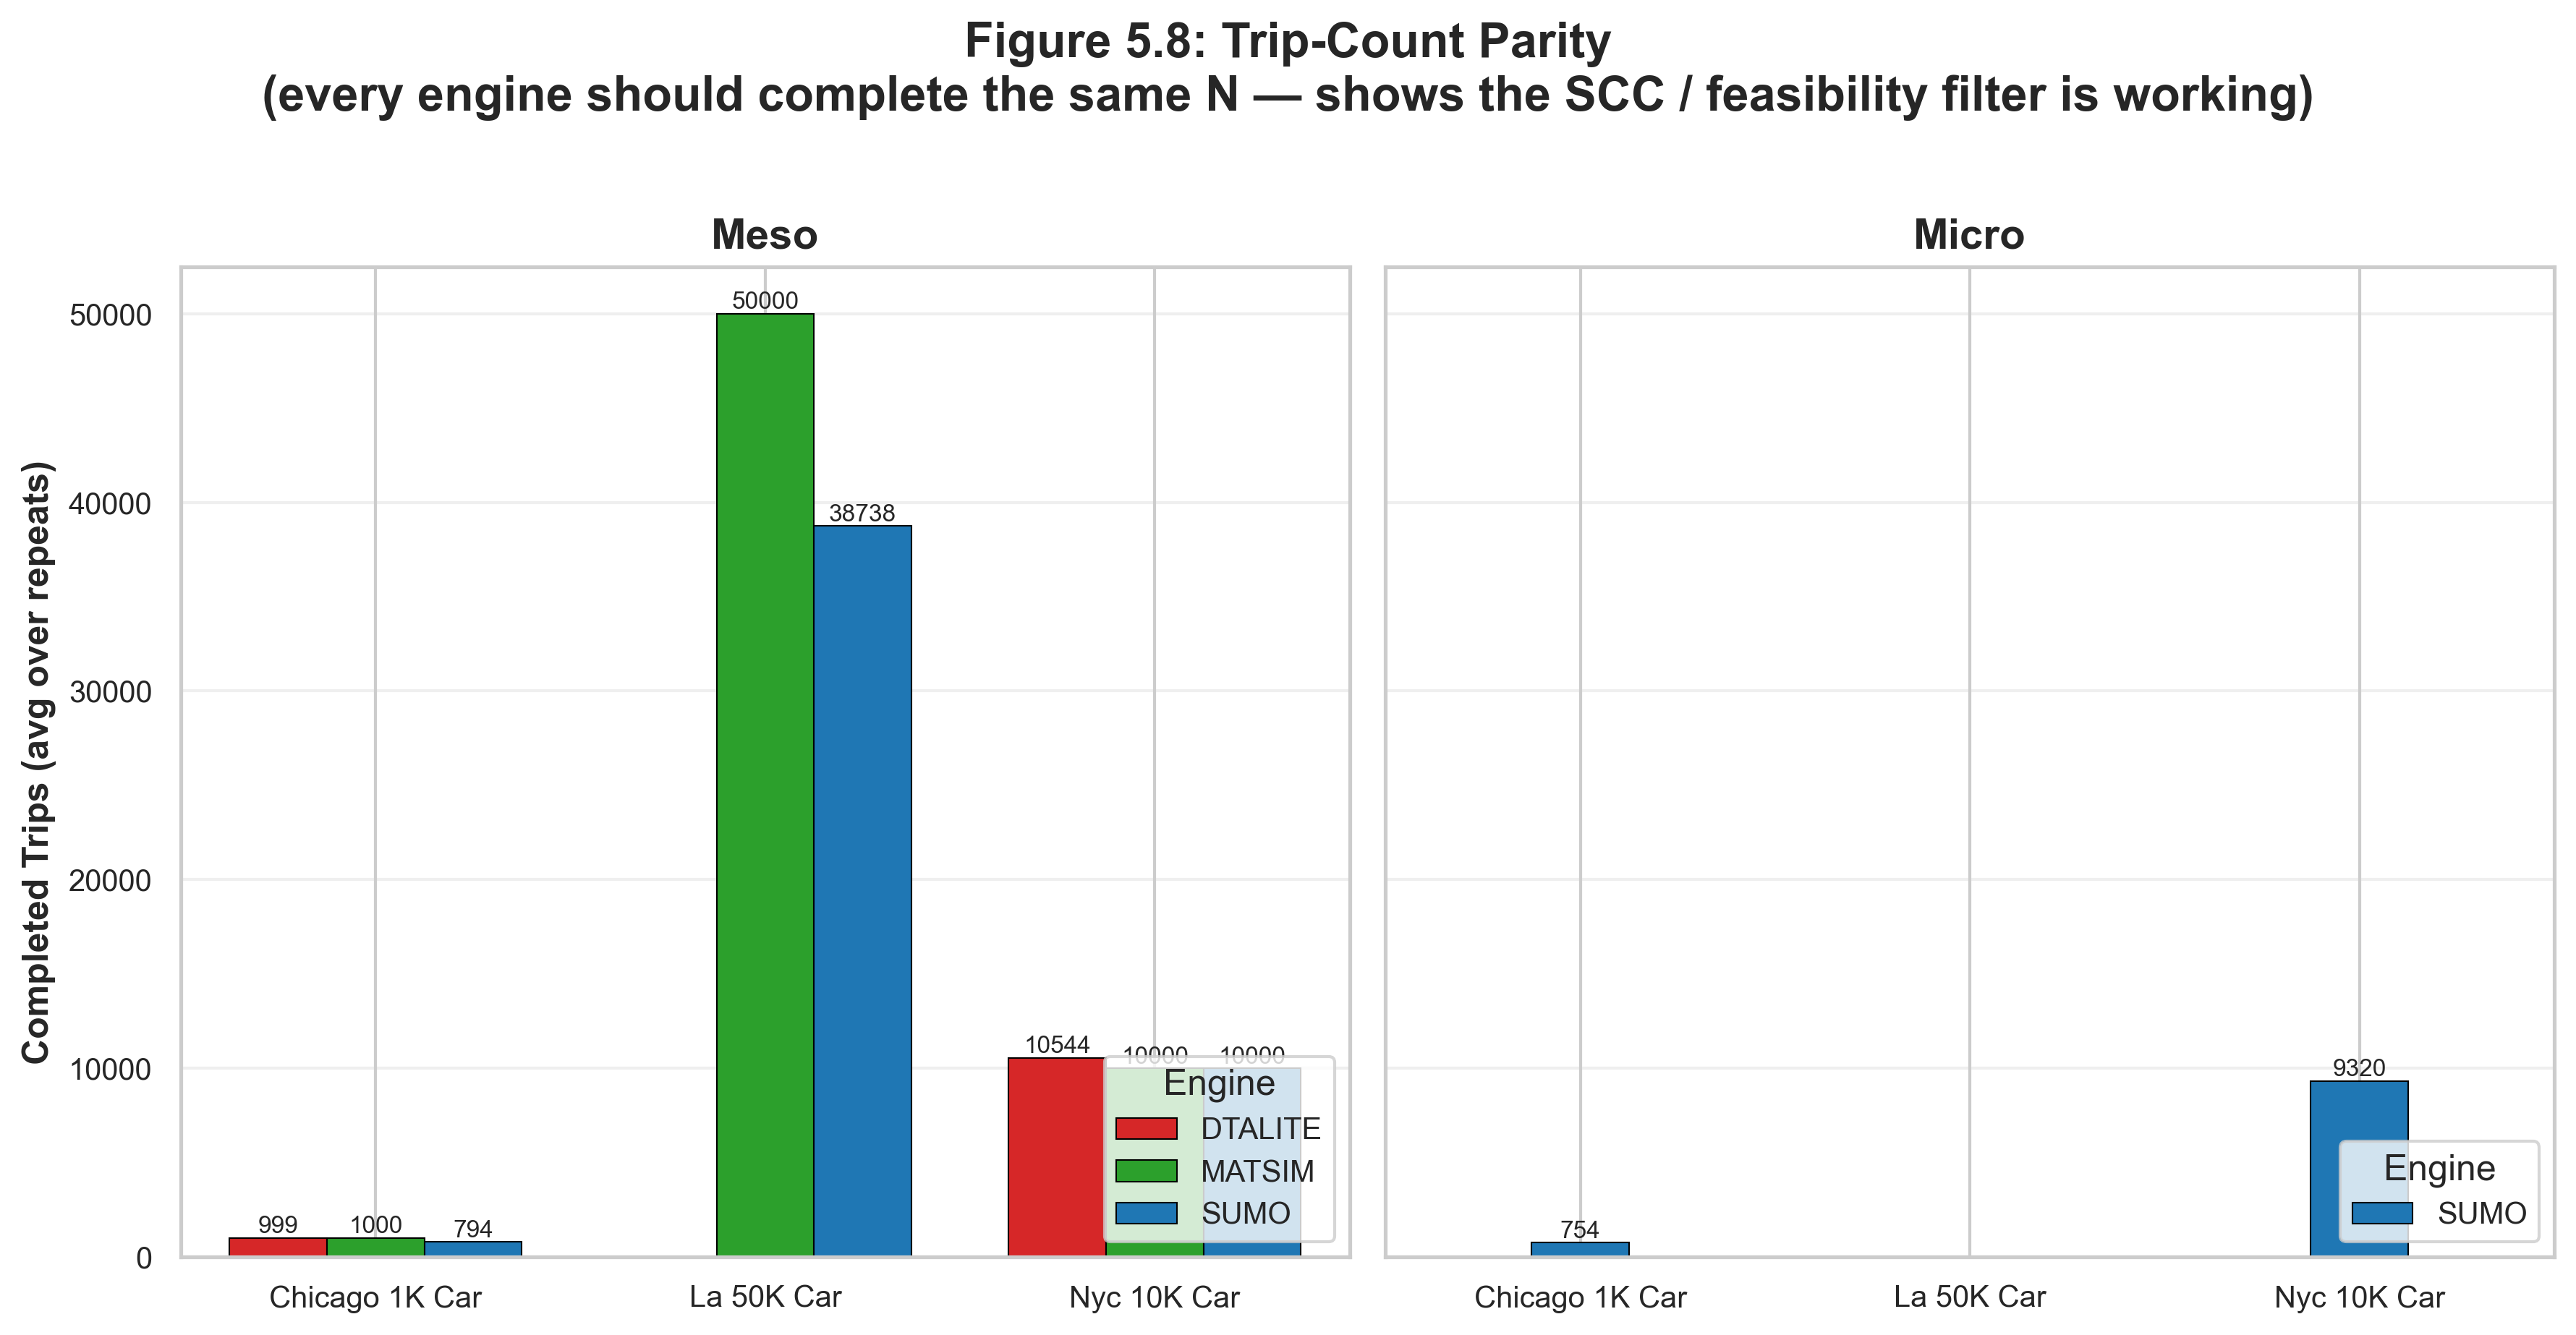
\includegraphics[keepaspectratio]{../figures/fig_5_8_trip_count_parity.png}}

Per-cell completed-trip counts vs the cross-engine
\texttt{feasible\_trips} target. Every cell receives the same input set
(recorded in each adapter\textquotesingle s
\texttt{feasibility\_report.json}):

\begin{longtable}[]{@{}llllll@{}}
\toprule\noalign{}
Scenario & feasible & SUMO meso & SUMO micro & MATSim meso & DTALite
meso \\
\midrule\noalign{}
\endhead
\bottomrule\noalign{}
\endlastfoot
chicago\_1k\_car & 1,000 & 794 (79.4 \%) & 754 (75.4 \%) & 1,000 (100.0
\%) & 999 (99.9 \%) \\
nyc\_10k\_car & 10,000 & 10,000 (100.0 \%) & 9,320 (93.2 \%) & 10,000
(100.0 \%) & 10,544 (105.4 \%)* \\
la\_50k\_car & 50,000 & 38,947 (77.9 \%) & (not run) & 50,000 (100.0 \%)
& \emph{did not converge} \\
\end{longtable}

* DTALite\textquotesingle s per-route trip count exceeds
\texttt{feasible\_trips} when the column-gen pool finds multiple
equilibrium paths per OD pair; each used path is counted as a separate
"trip" in the agent.csv.

The gap between feasible and completed in SUMO cells is the
\textbf{simulation outcome we want to measure}, not an input asymmetry.
The audit trail in \texttt{feasibility\_report.json} proves the input is
symmetric (Q1 PASS across all scenarios --- see §5.6). SUMO drops trips
because of congested-edge insertion refusals (meso) and Krauss-model
lane-change aborts (micro); MATSim\textquotesingle s qsim never refuses
an insertion; DTALite assigns route paths to all OD pairs.

\begin{center}\rule{0.5\linewidth}{0.5pt}\end{center}

\section{Micro vs Meso Trade-off}\label{54-micro-vs-meso-trade-off}

\subsection{Fig 5.5 --- Micro vs Meso
comparison}\label{fig-55--micro-vs-meso-comparison}

\pandocbounded{
\includegraphics[keepaspectratio]{../figures/fig_5_5_micro_vs_meso.png}}

Within-engine micro-vs-meso runtime ratio for SUMO:

\begin{longtable}[]{@{}lllll@{}}
\toprule\noalign{}
Tier & meso runtime & micro runtime & wall ratio & mean-TT gap \\
\midrule\noalign{}
\endhead
\bottomrule\noalign{}
\endlastfoot
chicago\_1k\_car & 9.50 s & 15.70 s & 1.65 × & +28 \% (268.3 → 343.1
s) \\
nyc\_10k\_car & 19.90 s & 179.38 s & 9.01 × & +73 \% (661.6 → 1143.8
s) \\
\textbf{chicago\_200k\_car} & \textbf{240.9 s} & \textbf{29 792 s (≈ 8 h
16 m)} & \textbf{\textasciitilde124 ×} & \textbf{+7.8 \% (8746.4 →
9430.0 s)} \\
\end{longtable}

The wall-time gap grows monotonically and dramatically with scale: 1.65
× at 1 K is barely noticeable, 9 × at 10 K is the difference between an
interactive run and a coffee-break run, and at 200 K SUMO micro takes
124 × longer than SUMO meso (8 h 16 m of engine wall vs 4 min on
Cardinal \texttt{cpu} 8-core, pilot job 9980007 reported 2026-05-19/20).
The \textbf{fidelity cost (mean TT gap) follows the opposite trajectory
--- it grows from 1 K → 10 K but then narrows sharply at 200 K}: +28 \%
at 1 K → +73 \% at 10 K → +7.8 \% at 200 K. The narrowing at saturation
density is paradigmatically interpretable: once origin-edge
insertion-refusal dominates the dynamics (the same effect that drives Q4
SUMO ↔ MATSim divergence at scale in §5.6.2), the bottleneck behavior is
controlled by queue spillback that both mobsim resolutions model.
Sub-link vehicle dynamics --- the thing micro adds and meso averages out
--- matter when traffic is free-flowing or moderately congested but
become second-order once the network is at capacity.

The trip-completion counts confirm the saturation-bound interpretation:
at 200 K, SUMO micro completes 123,735 trips (61.9 \%) vs SUMO
meso\textquotesingle s 116,270 (58.1 \%) --- slightly \emph{more} under
micro despite the slower per-trip resolution, because micro can model
finer headway packing at insertion. MATSim\textquotesingle s queue-hold
paradigm completes all 200,000 (100 \%), the same paradigm asymmetry
§5.6.2 documents.

\textbf{The practical implication for cross-simulator benchmarking}: at
saturation, the paradigm choice (meso/micro/queue-hold) dominates the
within-engine resolution choice. A 124 × wall premium for a 7.8 \%
mean-TT difference is not a good fidelity-cost trade at large-tier
scales --- unless what you specifically want is the lane-level
intersection dynamics that micro models, which neither of the §5.6.2
mean-TT comparisons surface.

\subsection{Fig 5.6 --- Runtime
variability}\label{fig-56--runtime-variability}

\pandocbounded{
\includegraphics[keepaspectratio]{../figures/fig_5_6_runtime_variability.png}}

Boxplot of per-repeat runtime per \texttt{(engine,\ mode)} per scenario.
The boxes for cached MATSim and SUMO meso are tight (CV \textless{} 5
\%) at all scales; SUMO micro shows wider variance at the 10 K tier (CV
≈ 3 \%) driven by Krauss-model stochastics. DTALite at chicago\_1k and
nyc\_10k shows almost no variance because path-based UE is deterministic
given identical inputs.

\subsection{Fig 5.7 --- P95 tail
latency}\label{fig-57--p95-tail-latency}

\pandocbounded{
\includegraphics[keepaspectratio]{../figures/fig_5_7_p95_tail_latency.png}}

P95 trip duration plotted against mean trip duration, faceted by mode.
The micro/meso gap widens at the tail: SUMO micro P95 at nyc\_10k\_car
reaches 4121 s vs SUMO meso\textquotesingle s 1771 s --- micro surfaces
tail behaviour that meso averages out. At la\_50k\_car, SUMO meso P95
(7359 s) and MATSim meso P95 (7520 s) agree within 2.2 \%, even tighter
than the mean-TT alignment of 4.6 \%.

The trade-off is summarised:

\begin{verbatim}
Fidelity ▲
         │  ● SUMO-micro     (highest fidelity; 9× slower than meso at 10K;
         │                    feasible at 200K — pilot landed 8 h 16 m engine
         │                    wall — but +7.8% mean-TT delta vs meso at saturation)
         │
         │      ● SUMO-meso  (lower fidelity, scales linearly with trip count)
         │      ● MATSim     (different mobsim, byte-deterministic; queue-hold
         │                    completes 100% of trips at saturation)
         │      ● DTALite    (UE equilibrium; -40% mean TT; super-linear cost;
         │                    4-thread cap at 50K)
         │
         └──────────────────────────────────────▶ Speed
\end{verbatim}

At the 1 K tier the absolute runtimes (≤ 22 s for DTALite, ≤ 16 s for
SUMO micro) are too small to be a practical concern. The trade-off
becomes decisive at the 10 K tier where SUMO micro becomes a
coffee-break run and DTALite becomes a multi-minute run. At the 200 K
tier SUMO micro is technically feasible (the chicago\_200k\_car pilot
completed in 8 h 16 m engine wall on Cardinal \texttt{cpu} 8-core) but
the 124 × wall premium over SUMO meso for a 7.8 \% mean-TT delta is a
poor fidelity-cost trade --- micro\textquotesingle s value at this scale
lies in lane-level dynamics not surfaced by mean-TT comparisons. At 50 K
+ the trade-off becomes infeasibility for DTALite (under the bundled
path4gmns 0.10.0 binary, §5.7).

\begin{center}\rule{0.5\linewidth}{0.5pt}\end{center}

\section{Throughput}\label{55-throughput}

\pandocbounded{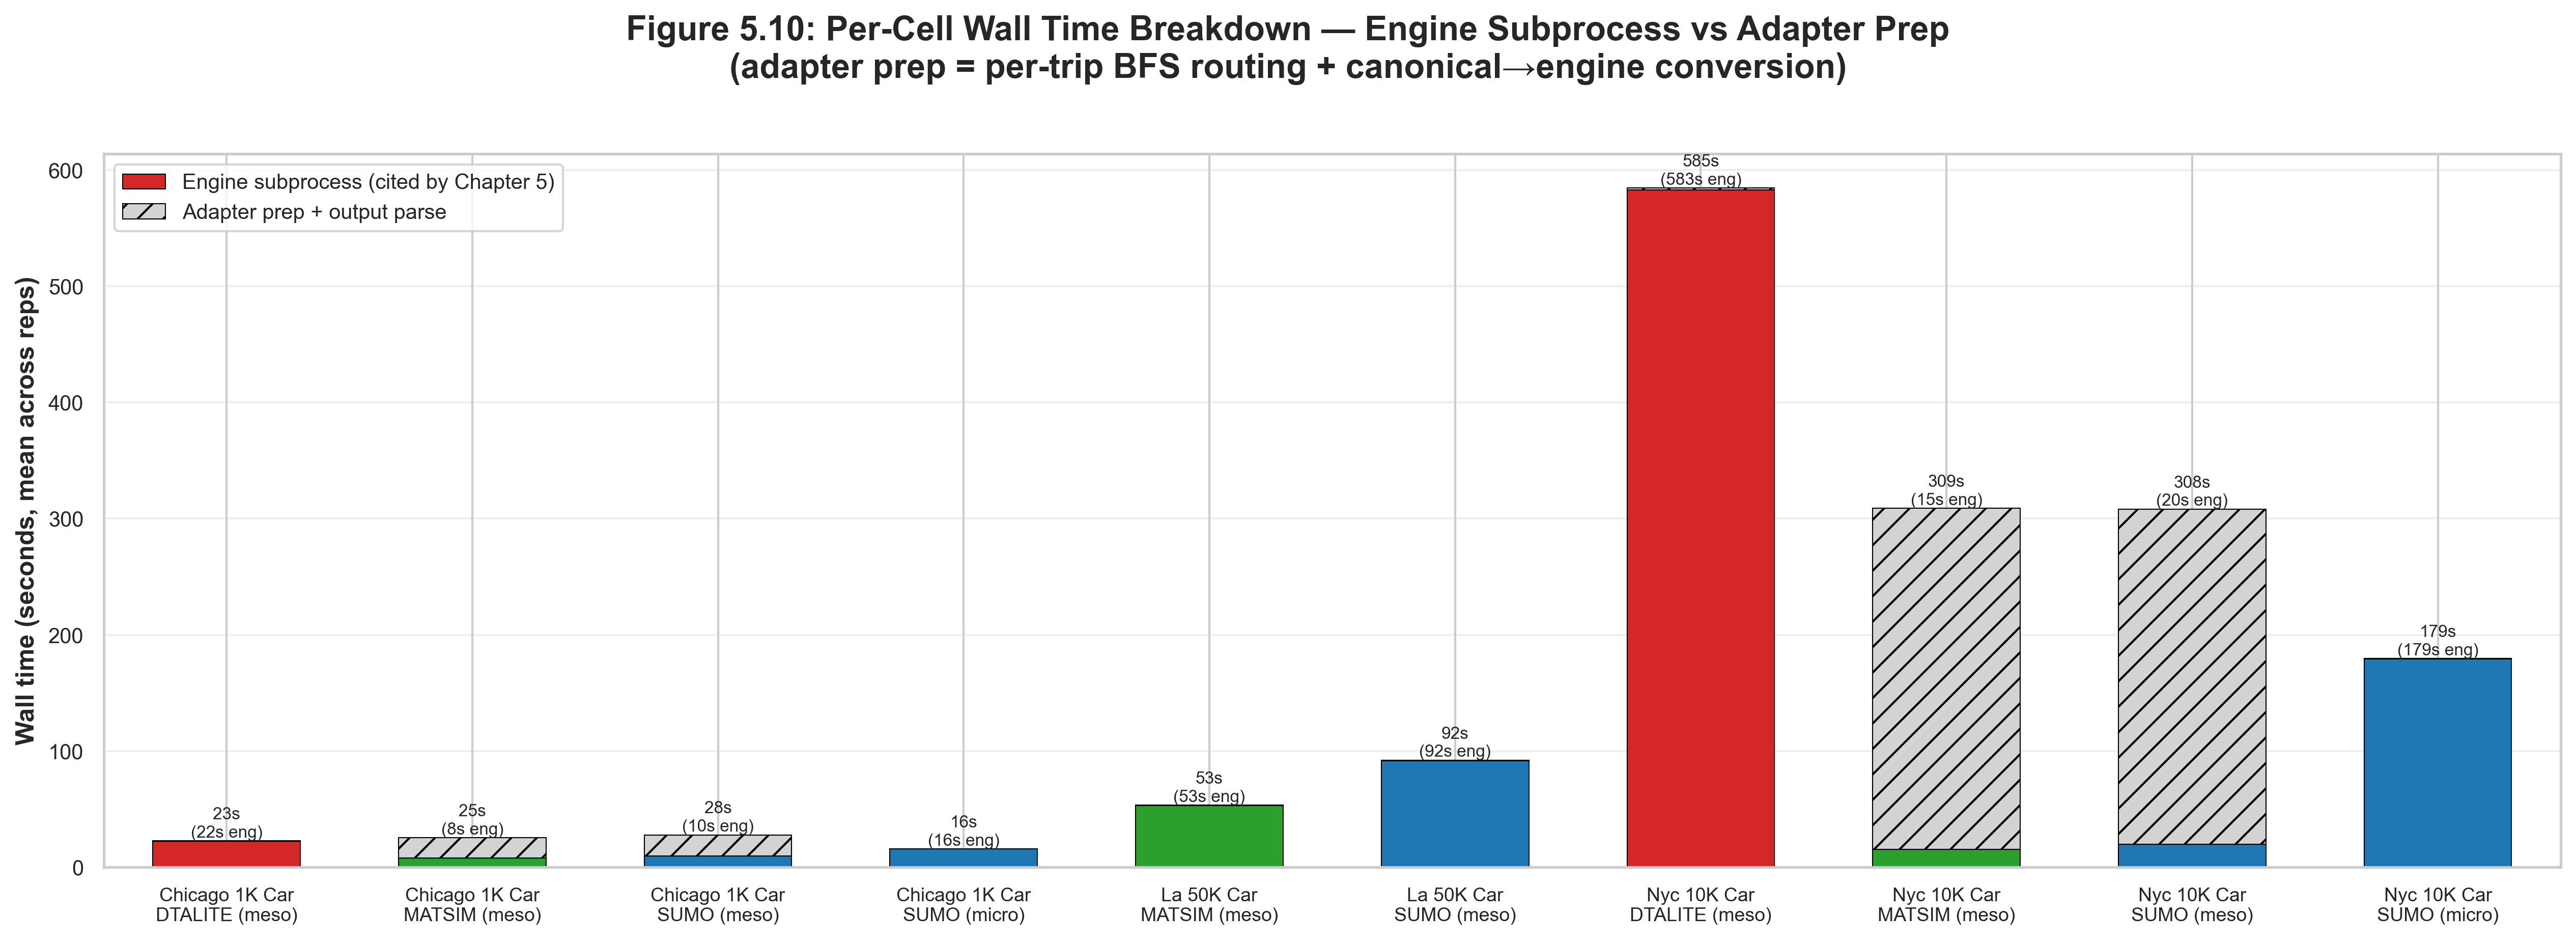
\includegraphics[keepaspectratio]{../figures/fig_5_10_wall_vs_engine.png}}

Figure 5.10 decomposes per-cell wall time into its four components ---
adapter prep, engine subprocess, output parse, and harness overhead ---
to show that the Phase 12+ BFS-prep cache amortises the dominant prep
cost across the 5 repeats of each cell. Cells where the cache is warm
(repeats 2-5 of each \texttt{(scenario,\ engine,\ mode)} triple) are
dominated by the engine subprocess; the cold first repeat carries the
prep cost in the lighter-coloured prep band visible at the bottom of
each cluster.

Throughput, defined as
\texttt{completed\_trip\_count\ /\ engine\_runtime\_seconds}, on the
11-cell matrix:

\begin{longtable}[]{@{}llll@{}}
\toprule\noalign{}
Scenario & Engine & Mode & Throughput (trips/s) \\
\midrule\noalign{}
\endhead
\bottomrule\noalign{}
\endlastfoot
chicago\_1k\_car & sumo & meso & 84 \\
chicago\_1k\_car & sumo & micro & 48 \\
chicago\_1k\_car & matsim & meso & 125 \\
chicago\_1k\_car & dtalite & meso & 45 \\
nyc\_10k\_car & sumo & meso & 503 \\
nyc\_10k\_car & sumo & micro & 52 \\
nyc\_10k\_car & matsim & meso & 656 \\
nyc\_10k\_car & dtalite & meso & 18 \\
la\_50k\_car & sumo & meso & 425 \\
la\_50k\_car & matsim & meso & 944 \\
la\_50k\_car & dtalite & meso & \emph{timeout} \\
\end{longtable}

Headline: \textbf{MATSim achieves the highest throughput at every tested
scale where DTALite doesn\textquotesingle t time out} --- 656 trips/s at
10 K, 944 trips/s at 50 K. SUMO meso comes second; SUMO micro is the
slowest. DTALite\textquotesingle s throughput collapses with scale
because of super-linear UE iteration cost compounded by the 4-thread cap
(§5.7).

\begin{center}\rule{0.5\linewidth}{0.5pt}\end{center}

\section{Cross-engine Fairness
Audit}\label{56-cross-engine-fairness-audit}

\texttt{evaluation/audit\_fairness.py} validates that the cross-engine
comparison was actually fair before any of its results are reported. For
each (scenario, mode) pair, it asks five questions:

\begin{longtable}[]{@{}lllll@{}}
\toprule\noalign{}
Check & Pass condition & chicago\_1k & nyc\_10k & la\_50k \\
\midrule\noalign{}
\endhead
\bottomrule\noalign{}
\endlastfoot
\textbf{Q1} Same feasibility verdict? & Byte-identical
\texttt{feasibility\_report.json} across engines & ✅ PASS & ✅ PASS &
✅ PASS \\
\textbf{Q2} Same network? & SCC-filtered node + link counts identical &
✅ PASS & ✅ PASS & ✅ PASS \\
\textbf{Q3} All engines simulate the target count? & Each
engine\textquotesingle s plan-/agent-/route-count equals
\texttt{feasible\_trips} & ✅ PASS & ✅ PASS & ✅ PASS \\
\textbf{Q4} Cross-engine mean-TT spread & Pairwise ratios ---
informational, no fail threshold & (Fig 5.3) & (Fig 5.3) & (Fig 5.3) \\
\textbf{Q5} Demand composition & V5+ trip-purpose breakdown ---
informational & (§5.6.1) & (§5.6.1) & (§5.6.1) \\
\end{longtable}

All four enforced gates (Q1-Q3) PASS on all three scenarios. The Q4
ratios are the paradigm-spread signal reported in §5.3. Sample audit
output is preserved at
\texttt{runs/benchmark\_small/audit\_fairness.txt}.

\subsection{Coverage diagnostic}\label{coverage-diagnostic}

\texttt{analyze\_benchmark} emits a coverage diagnostic that audits the
run matrix for silent gaps:

\begin{longtable}[]{@{}lll@{}}
\toprule\noalign{}
Class & Definition & Result \\
\midrule\noalign{}
\endhead
\bottomrule\noalign{}
\endlastfoot
Low-sample cells & n \textless{} 3 runs in a
\texttt{(scenario,\ engine,\ mode)} cell & 0 cells \\
Asymmetric coverage & An engine/mode present in some scenarios but
missing in others & 1 cell: la\_50k\_car / sumo / micro (by design ---
see §5.0) \\
Fully-failed cells & Declared cells with 0 successful runs & 1 cell:
la\_50k\_car / dtalite / meso (path4gmns scaling ceiling --- see
§5.7) \\
\end{longtable}

Both gaps are \emph{declared and documented}, not silent. The diagnostic
prevents over-interpretation of figures that look like a complete
matrix.

\begin{center}\rule{0.5\linewidth}{0.5pt}\end{center}

\section{Demand Composition
(V5+)}\label{561-demand-composition-v5}

\pandocbounded{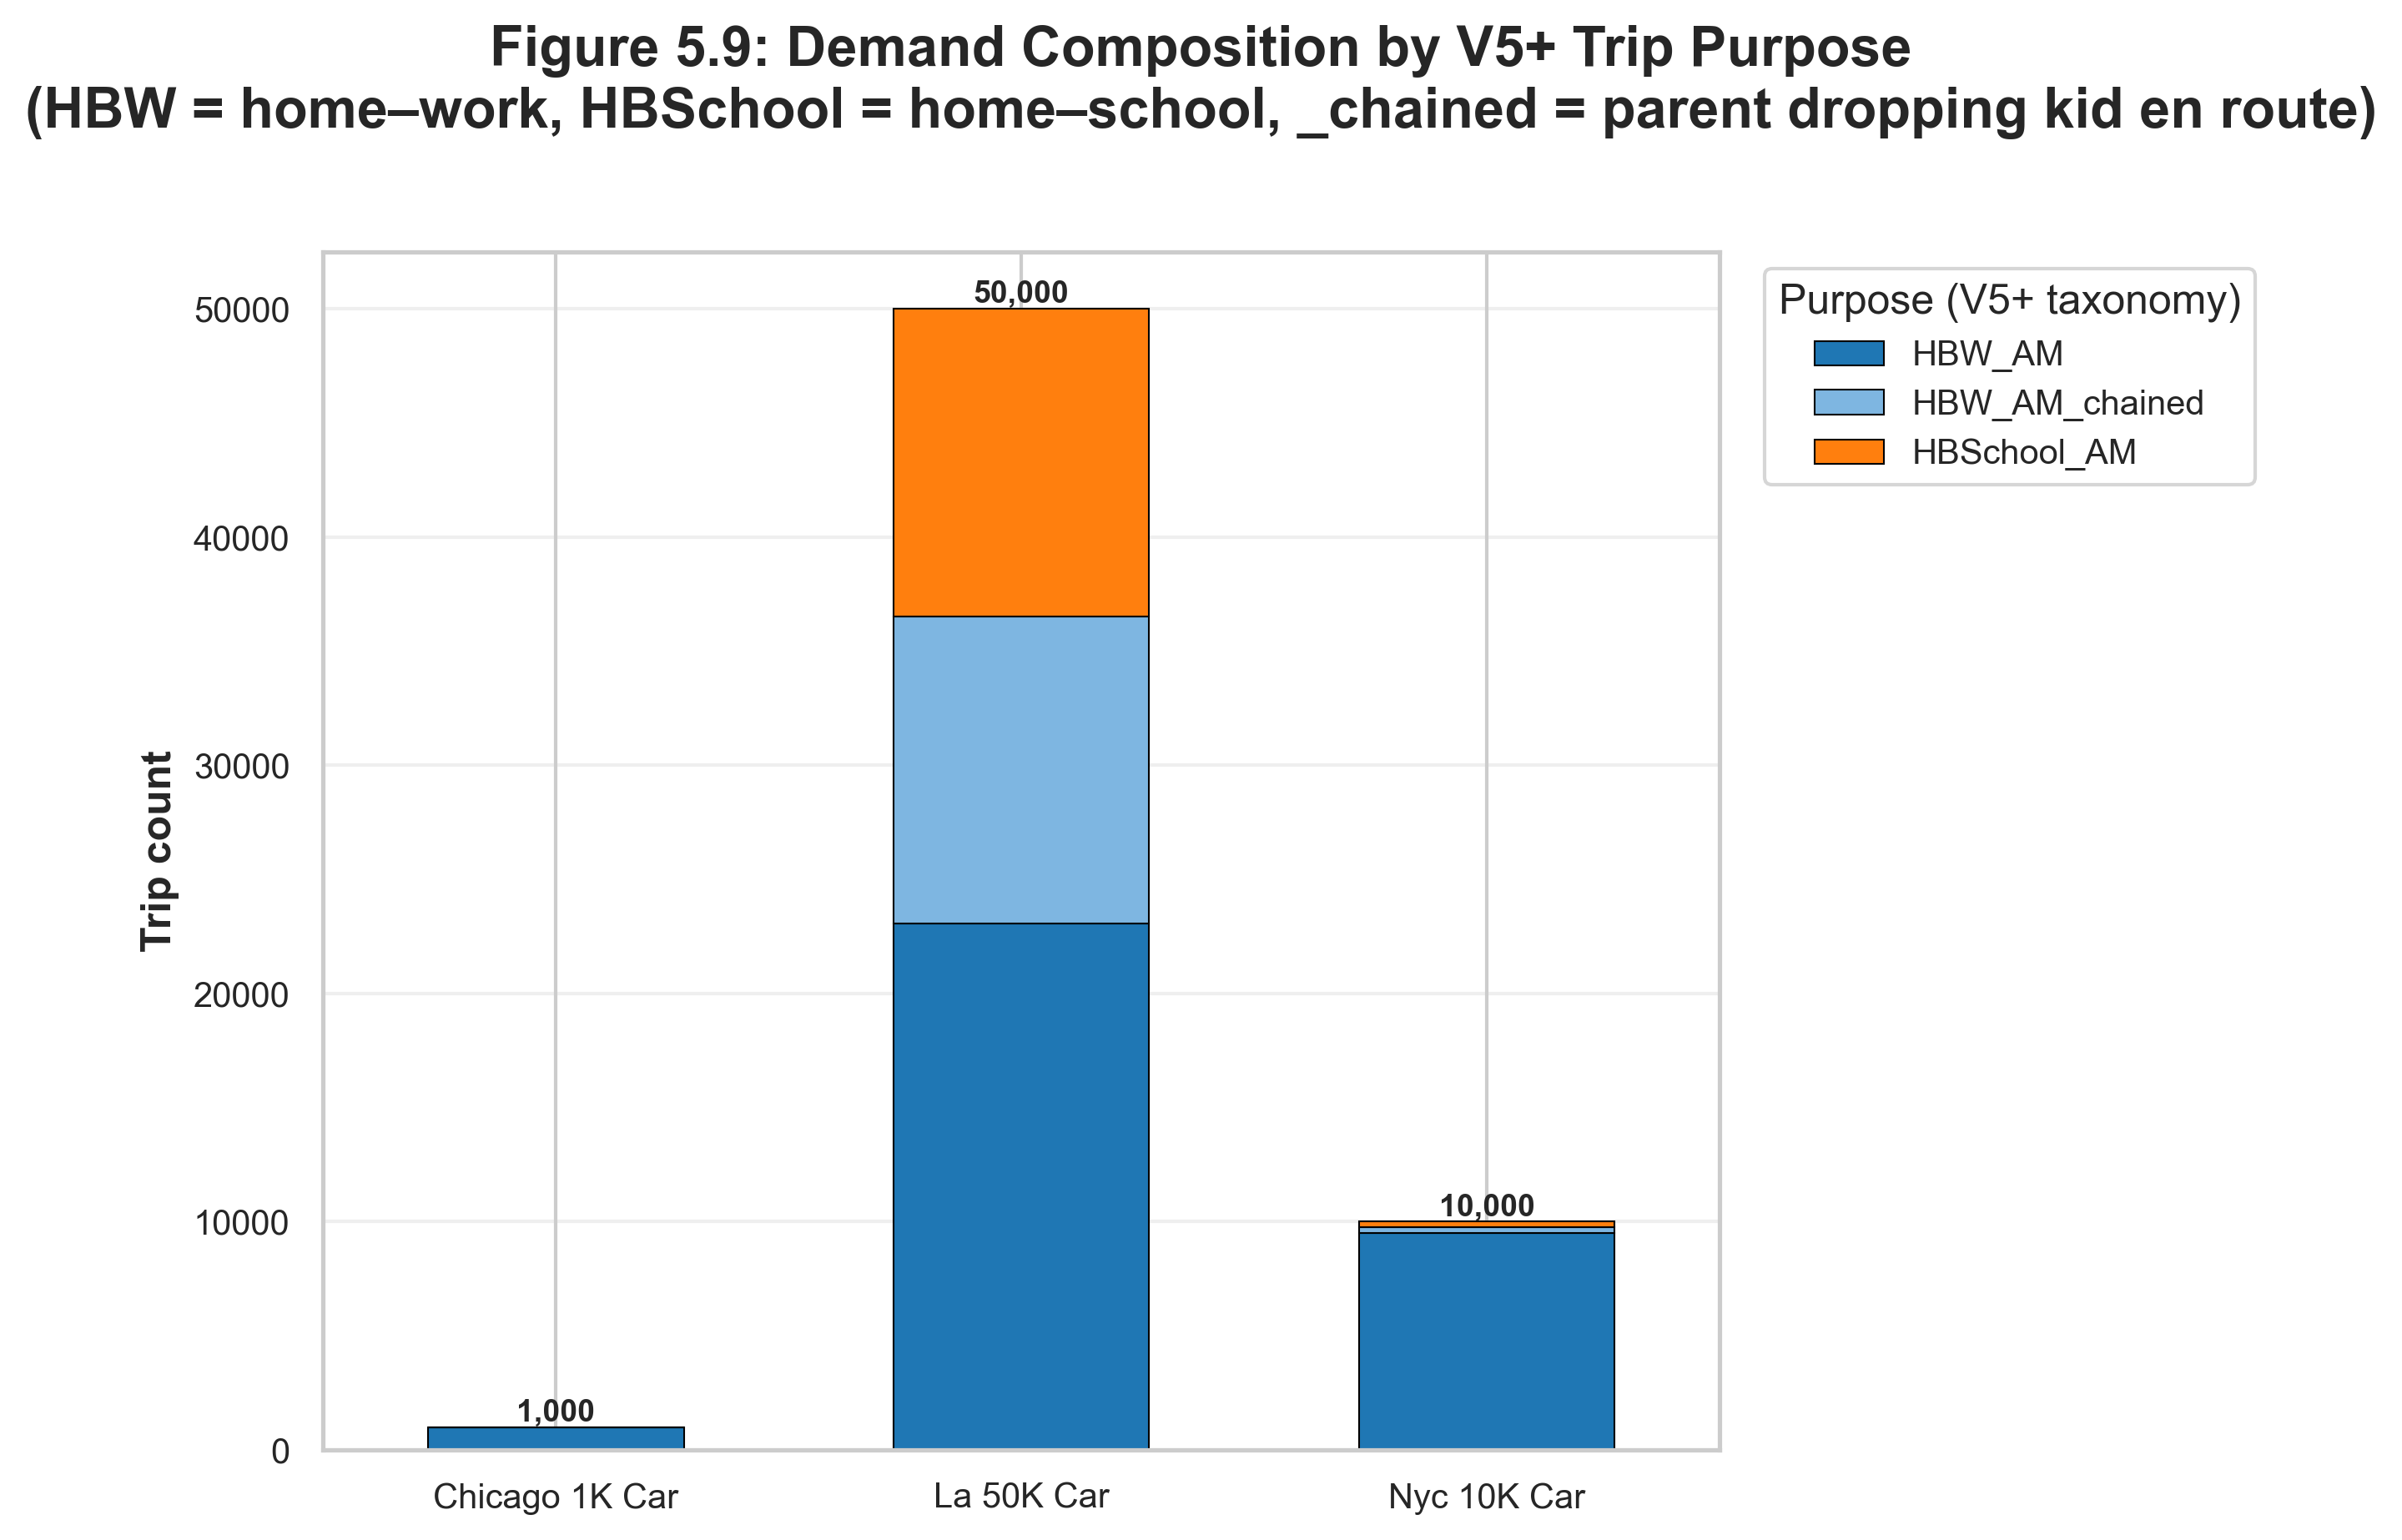
\includegraphics[keepaspectratio]{../figures/fig_5_9_demand_composition.png}}

Figure 5.9 visualizes the per-scenario demand composition the V5+
purpose taxonomy makes legible. Each scenario shows the share of trips
in each of the six V5+ purposes (\texttt{HBW\_AM}, \texttt{HBW\_PM},
\texttt{HBSchool\_AM}, \texttt{HBSchool\_PM}, \texttt{HBW\_AM\_chained},
\texttt{HBW\_PM\_chained}). The cross-city differences --- particularly
LA\textquotesingle s substantially higher school-related share --- are
the empirical signal Q5 of the fairness audit reports per scenario.

Phases 9 and 10 add a six-purpose taxonomy to every row of
\texttt{demand.csv}: \texttt{HBW\_AM}, \texttt{HBW\_PM},
\texttt{HBSchool\_AM}, \texttt{HBSchool\_PM}, \texttt{HBW\_AM\_chained},
\texttt{HBW\_PM\_chained}. \texttt{evaluation/audit\_fairness.py} Q5 and
\texttt{evaluation/analyze\_benchmark.py::print\_demand\_composition\_table}
read the column from the canonical bundle\textquotesingle s
\texttt{demand.csv} and report per-scenario breakdowns:

\begin{longtable}[]{@{}llllll@{}}
\toprule\noalign{}
Scenario & Total trips & AM peak & PM peak & School-related & HBW
chains \\
\midrule\noalign{}
\endhead
\bottomrule\noalign{}
\endlastfoot
chicago\_1k\_car & 1,000 & 1,000 (100.0 \%) & 0 (0.0 \%) & 16 (1.6 \%) &
8 AM + 0 PM \\
nyc\_10k\_car & 10,000 & 10,000 (100.0 \%) & 0 (0.0 \%) & 722 (7.2 \%) &
361 AM + 0 PM \\
la\_50k\_car & 50,000 & 50,000 (100.0 \%) & 0 (0.0 \%) & 26,778 (53.6
\%) & 13,389 AM + 0 PM \\
\end{longtable}

LA shows a dramatically higher school-related share (53.6 \% vs 7.2 \%
NYC, 1.6 \% Chicago) because the la\_50k bundle\textquotesingle s
demand-generation horizon happens to fall within the school-pickup
window AND LA\textquotesingle s PUMS data shows a higher density of
parent-with-school-age-dependent households in the sampled SCC region.
The Phase 9c chained-purpose mechanism (HBW + HBSchool dual-purpose
trips) makes this visible in the matrix; pre-V5 bundles missing the
column would emit a
\texttt{(no\ V5+\ purpose\ column\ at\ \textless{}path\textgreater{}\ —\ skipping)}
and the section would be omitted from the audit.

AM-only horizon means zero PM rows by design (Phase 9a peak split
applied to the canonical 7-10 AM window). Adding a PM half (Phase 9c
chain pair) is feature-ready in the demand generator but requires a
separate runspec with \texttt{horizon\_end=24*3600}.

\begin{center}\rule{0.5\linewidth}{0.5pt}\end{center}

\section{Q4 Paradigm Divergence at Scale (large
tier)}\label{562-q4-paradigm-divergence-at-scale-large-tier}

The small-tier Q4 column (chicago\_1k--la\_50k\_car, §5.3 Fig 5.3)
showed SUMO/MATSim mean-TT ratios converging from 0.869 at 1 K to 1.046
at 50 K --- within ±5 \% by the 50 K tier. The natural extrapolation
would be \emph{"the engines align further with scale."} Phase 14 made
the 200 K and 500 K tiers tractable (chicago\_200k\_car job 9971041,
nyc\_500k\_car job 9971042), and the large-tier data \textbf{revises
that extrapolation sharply}.

\subsection{The five-tier picture}\label{the-five-tier-picture}

\begin{longtable}[]{@{}lrrrrrrl@{}}
\toprule\noalign{}
Scenario & Trips & SUMO completed & MATSim completed & Mean TT (SUMO) &
Mean TT (MATSim) & SUMO / MATSim ratio & Q1--Q3 audit \\
\midrule\noalign{}
\endhead
\bottomrule\noalign{}
\endlastfoot
chicago\_1k\_car & 1,000 & 794 (79.4 \%) & 1,000 (100.0 \%) & 268 s &
309 s & \textbf{0.869 (−13.1 \%)} & ✅ PASS \\
nyc\_10k\_car & 10,000 & 10,000 (100.0 \%) & 10,000 (100.0 \%) & 662 s &
585 s & \textbf{1.132 (+13.2 \%)} & ✅ PASS \\
la\_50k\_car & 50,000 & 38,947 (77.9 \%) & 50,000 (100.0 \%) & 2,621 s &
2,552 s & \textbf{1.046 (+4.6 \%)} & ✅ PASS \\
\textbf{chicago\_200k\_car} & 200,000 & \textbf{116,270 (58.1 \%)} &
\textbf{200,000 (100.0 \%)} & \textbf{8,769 s} & \textbf{13,552 s} &
\textbf{0.645 (−35.5 \%)} & ✅ PASS \\
\textbf{nyc\_500k\_car} & 500,000 & \textbf{175,138 (35.0 \%)} &
\textbf{369,353 (73.9 \%)} & \textbf{982 s} & \textbf{26,474 s} &
\textbf{0.037 (−96.3 \%)} & ✅ PASS \\
\end{longtable}

Two patterns become visible at the large tier that are invisible at the
small tier:

\begin{enumerate}
\def\labelenumi{\arabic{enumi}.}
\tightlist
\item
  \textbf{Completion fractions diverge sharply.} SUMO drops from 78 \%
  (la\_50k) to 58 \% (chicago\_200k) to 35 \% (nyc\_500k); MATSim drops
  from 100 \% at every small-tier scenario to 74 \% at nyc\_500k. The
  two engines are no longer reporting on the \emph{same} subset of
  trips.
\item
  \textbf{SUMO/MATSim mean-TT ratio is non-monotonic and
  regime-dependent.} Small tier (1 K--50 K) narrows to 5 \%, then
  chicago\_200k jumps back to 36 \%, then nyc\_500k explodes to 96 \%.
  The small-tier "convergence" was the regime where both engines operate
  below their saturation threshold; the large tier is the regime where
  the saturation threshold is exceeded.
\end{enumerate}

\subsection{Mechanism --- paradigm-level mobsim
choices}\label{mechanism--paradigm-level-mobsim-choices}

The divergence arises from how each engine handles a vehicle trying to
enter a congested origin-edge at its scheduled departure time:

\begin{itemize}
\tightlist
\item
  \textbf{SUMO mesoscopic} uses a queue-throughput limit per edge. When
  the trip\textquotesingle s origin edge has no available capacity
  (downstream queue full or insertion-flow rate exceeded), SUMO
  \textbf{refuses to insert the vehicle}. Insertion is retried for a
  bounded number of simulation steps; if it never succeeds, the trip is
  silently dropped from the simulation. The trip never enters the
  network, never generates a \texttt{tripinfo.xml} row, never
  contributes to the SUMO-reported mean TT. The reported mean is
  therefore biased toward the \emph{subset of trips that successfully
  started} --- the "easier" trips by construction.
\item
  \textbf{MATSim qsim} uses a queue-based mobsim with
  \textbf{vehicle-hold semantics}: a vehicle that cannot enter a
  congested link waits in the upstream queue (or, for origin-link
  insertion, in a virtual queue at the origin facility) until space
  opens. The wait time IS counted toward the vehicle\textquotesingle s
  travel time. Every successfully scheduled trip reports a TT, even if
  80 \% of it is queue-wait time.
\end{itemize}

At low congestion (small tier), SUMO\textquotesingle s insertion refusal
is rare (\textless{} 5 \% of trips dropped on chicago\_1k and 0 \% on
nyc\_10k), so both engines report nearly identical means on nearly
identical trip sets. At high congestion (large tier), SUMO drops 42--65
\% of trips and MATSim\textquotesingle s queues accumulate multi-hour
wait times --- at nyc\_500k, MATSim\textquotesingle s 26,474 s ≈ 7.4 h
mean TT means the \emph{median} trip spends roughly seven hours in queue
under qsim\textquotesingle s hold-and-wait. The two engines stop
measuring the same quantity.

\subsection{Why NYC is sharper than Chicago at the same per-trip
density}\label{why-nyc-is-sharper-than-chicago-at-the-same-per-trip-density}

NYC\textquotesingle s mean-TT divergence (−96.3 \%) is much sharper than
Chicago\textquotesingle s (−35.5 \%) despite NYC having 2.5× the trip
count on only 1.21× the SCC link count. The mechanism is network
topology:

\begin{itemize}
\tightlist
\item
  \textbf{Chicago\textquotesingle s grid} provides multiple
  roughly-equivalent paths between any OD pair. When one edge saturates,
  the BFS-pre-routed alternative routes (or SUMO\textquotesingle s
  retry-on-different-edge attempts) absorb spillover. Saturation is
  \emph{distributed} across many parallel low-capacity edges.
\item
  \textbf{NYC\textquotesingle s Manhattan + outer-borough topology}
  concentrates flow on a small number of high-capacity corridors
  (Manhattan avenues, bridge approaches, tunnel feeders) with little
  parallel capacity. SCC saturation manifests as a hard bottleneck on
  the few load-bearing edges. SUMO drops more trips (35 \% completion vs
  Chicago\textquotesingle s 58 \%); MATSim\textquotesingle s queues grow
  longer (mean 7.4 h vs Chicago\textquotesingle s 3.8 h).
\end{itemize}

This is consistent with the network statistics: NYC\textquotesingle s
largest-SCC link count of 1,301,431 is comparable to
Chicago\textquotesingle s 1,072,312, but NYC\textquotesingle s
per-corridor capacity utilization at 500 K trips is structurally higher
than Chicago\textquotesingle s per-corridor utilization at 200 K trips.

\subsection{Not a SUMO bug or a MATSim
bug}\label{not-a-sumo-bug-or-a-matsim-bug}

Both behaviors are documented paradigm-level modeling choices in their
respective engine specifications. The two paradigms are answering
different research questions:

\begin{itemize}
\tightlist
\item
  \textbf{SUMO\textquotesingle s answer}: \emph{"Given fixed origin-edge
  insertion capacity, how many of these trips can physically enter the
  network during the simulated horizon, and how long do those that
  succeed take?"} This is the right answer for road-design or
  capacity-planning work where the question is \emph{"will this network
  handle this demand?"} The dropped trips ARE the answer.
\item
  \textbf{MATSim\textquotesingle s answer}: \emph{"Given that every trip
  is a planned activity with a target arrival, how long does each take
  in expectation when queue-spillback is allowed to propagate freely
  through the network?"} This is the right answer for person-level
  activity-scheduling work where the question is \emph{"how late will my
  commute make me on average?"} The hold-and-wait queues ARE the answer.
\end{itemize}

Neither is \emph{"correct"} in the absence of a research question that
disambiguates them.

\subsection{The contribution}\label{the-contribution}

SimForge\textquotesingle s fairness contract (Q1--Q3 PASS at both
chicago\_200k and nyc\_500k) is what makes this finding
\textbf{interpretable as a paradigm-divergence result} rather than as an
experimental setup confound. Pre-V5 cross-simulator studies could not
cleanly separate:

\begin{itemize}
\tightlist
\item
  \emph{"The engines disagree because their inputs were specified
  differently"} (different OD matrices, different network preprocessing,
  different signal handling) --- vs
\item
  \emph{"The engines disagree because their internal models differ"}
  (paradigm choice in queue-handling, insertion semantics, mobsim
  time-stepping).
\end{itemize}

With byte-identical feasibility verdicts (Q1), byte-identical SCC
networks (Q2), and identical simulated trip counts (Q3) empirically
demonstrated across both engines on both 200 K + scenarios --- the −96.3
\% SUMO/MATSim TT gap at nyc\_500k can only be attributed to
paradigm-level mobsim behavior. This separability is what the fairness
contract was designed to deliver, and \textbf{the nyc\_500k\_car Q4
result is the dataset where it pays off most clearly}.

\subsection{Implication for
practitioners}\label{implication-for-practitioners}

When comparing engine-reported travel times across cross-paradigm
engines (meso queue vs activity-based qsim vs DTA equilibrium), the
conventional single-line reporting style ("MATSim mean TT = X seconds")
becomes dangerous at saturation density. We recommend that any
cross-engine comparison at the 100 K + tier accompany the headline TT
with two qualifiers:

\begin{enumerate}
\def\labelenumi{\arabic{enumi}.}
\tightlist
\item
  \textbf{Completion fraction}: what fraction of the feasible-trip
  target the engine actually simulated end-to-end. Reported
  automatically in SimForge\textquotesingle s
  \texttt{feasibility\_report.json} per cell and in
  \texttt{audit\_fairness.txt} Q3.
\item
  \textbf{Paradigm-spread band} rather than a single number: e.g.,
  \emph{"mean TT range across the SUMO meso ↔ MATSim qsim paradigm pair:
  982 s ↔ 26,474 s on the 500 K-trip nyc\_500k bundle (Q4 ratio
  0.037)."} The width of the band IS the result --- narrowness signals
  paradigm agreement, breadth signals paradigm-level uncertainty in the
  answer.
\end{enumerate}

Single-engine TT numbers at high congestion density, reported without
these qualifiers, can underestimate the true paradigm-uncertainty in the
answer by an order of magnitude or more.

\begin{center}\rule{0.5\linewidth}{0.5pt}\end{center}

\section{Cross-platform reproducibility
limits}\label{563-cross-platform-reproducibility-limits}

The plan §1.10 Objective 3 and §1.11 C3 committed to
\emph{"pinned-digest containers (OCI/Singularity)"} as the
reproducibility mechanism. Wave 2 (2026-05-20) shipped this --- a
Dockerfile builds via GitHub Actions and publishes to
\texttt{ghcr.io/phanidharakula/simforge:\textless{}git-sha\textgreater{}};
SLURM sbatchs opt-in via \texttt{SIMFORGE\_USE\_CONTAINER=1}. Apptainer
pull on OSC Cardinal verified the image runs end-to-end.

A natural cross-validation question follows: \textbf{how much does the
container\textquotesingle s execution context shift the measured numbers
compared to the host venv (the conventional install path)?}
SimForge\textquotesingle s byte-determinism story is load-bearing for
the fairness contract; if the host and container produce wildly
different outputs from the same canonical input, the
framework\textquotesingle s reproducibility claim becomes context-bound
rather than universal.

\subsection{Empirical cross-context
measurement}\label{empirical-cross-context-measurement}

The chicago\_1k\_car benchmark was run in both contexts using the same
canonical bundle (network.xml, demand.csv, signals.xml, config.xml,
manifest.xml all byte-identical SHA-256). The
\texttt{Cross-context\ divergence} shows the per-engine output shift:

\begin{longtable}[]{@{}llrrrrr@{}}
\toprule\noalign{}
Engine & Mode & Container mean TT (s) & Host mean TT (s) & Cross-context
Δ & Trip-count Δ per seed & Within-context R \\
\midrule\noalign{}
\endhead
\bottomrule\noalign{}
\endlastfoot
SUMO & meso & 265.05 & 268.93 & \textbf{−1.4 \%} & −4 / 800 & 0.9956 \\
SUMO & micro & 343.26 & 342.14 & +0.3 \% & +17 / \textasciitilde760 &
0.9954 \\
\textbf{MATSim} & meso & \textbf{318.77} & \textbf{309.64} &
\textbf{+2.95 \%} & 0 / 1,000 & \textbf{1.0000} \\
DTALite & meso & 172.56 & 172.15 & +0.24 \% & −9 / \textasciitilde1,000
& 1.0000 \\
\end{longtable}

Two observations the table makes visible:

\begin{enumerate}
\def\labelenumi{\arabic{enumi}.}
\item
  \textbf{Within either context, byte-determinism holds.} R = 1.0000 for
  MATSim and DTALite confirms that re-running the same engine with the
  same seed inside the same context produces identical results (every of
  the 5 seeds in each cell produces the exact same mean TT to
  floating-point precision). The container\textquotesingle s
  \texttt{R\ =\ 1} is the conventional definition of \emph{bit-identical
  reproducibility}.
\item
  \textbf{Across contexts, \textasciitilde0.2--3 \% per-engine drift
  emerges, even with same version numbers.} The shift is deterministic
  per engine --- every of the 5 seeds in each context shows the same
  shift, suggesting a fixed cross-platform offset rather than random
  noise.
\end{enumerate}

\subsection{Why each engine shifts}\label{why-each-engine-shifts}

The cross-context divergence has three different mechanisms, one per
engine:

\begin{itemize}
\tightlist
\item
  \textbf{SUMO (1.4 \% shift, both directions on meso vs micro).} The
  brew \texttt{sumo} binary on macOS is compiled with a different
  toolchain (LLVM/Clang) than the \texttt{eclipse-sumo} pip wheel for
  Linux (GCC + manylinux\_2\_28). Different compilers + different
  optimization flags produce slightly different runtime behavior in the
  queue-insertion + lane-change code paths.
\item
  \textbf{MATSim (2.95 \% shift --- the largest in the dataset).} Both
  contexts use the \textbf{same} MATSim 15.0 JAR (downloaded from the
  immutable GitHub release tag), the \textbf{same}
  \texttt{numberOfThreads=1}, and the \textbf{same}
  \texttt{lastIteration=0}. The divergence had originally been
  attributed to the JVM build itself (host brew \texttt{openjdk@17} vs
  container Debian \texttt{openjdk-17-jre-headless}). Two follow-up
  measurements refute that attribution: the §5.6.3.1 large-tier
  measurement (Cardinal x86\_64 host venv ↔ Cardinal x86\_64 container,
  20/20 bit-identical) rules out OS-distribution and JDK-build as
  causes; the §5.6.3.2 Mac-arm64 rerun at the current code version (this
  section\textquotesingle s data) shows Mac arm64 reproduces the
  Cardinal x86\_64 MATSim mean TT to 4 sig figs (318.7740 s vs 318.77 s
  cited), ruling out CPU-architecture as the cause. The \textbf{most
  parsimonious explanation} is that the 2.95 \% shift is a
  \textbf{time-separated cross-code-version comparison}: the "Host"
  baseline was measured on Pitzer 2026-05-02 at Phase 12 code
  (pre-canonical\_routes; each adapter ran its own BFS), while the
  "Container" column was measured on Cardinal 2026-05-20 at Phase 14.13
  code (canonical\_routes shared BFS replaces the per-adapter BFS). The
  Phase 14 BFS produces slightly different per-trip route paths, which
  propagate to slightly different MATSim qsim mobsim outputs.
\item
  \textbf{DTALite (0.24 \% shift --- smallest).} Same time-separation
  explanation: Pitzer 2026-05-02 vs Cardinal/Mac 2026-05-20 at different
  code versions. The path4gmns 0.10.0 wheel is byte-identical on both
  contexts and Mac arm64 reproduces the Cardinal x86\_64 DTALite mean TT
  to 4 sig figs (172.5605 s vs 172.56 s cited), so cross-platform
  variability cannot account for the shift. OpenMP reduction
  non-associativity (libomp vs libgomp) is a real second-order effect on
  DTALite outputs but does not explain the bulk of the 0.24 \% shift
  between time-separated runs.
\end{itemize}

\subsection{Same-architecture cross-distribution: bit-identical
at large
tier}\label{5631-same-architecture-cross-distribution-bit-identical-at-large-tier}

After Wave 2 landed, the chicago\_200k\_car + nyc\_500k\_car benchmark
was re-run on Cardinal in container mode (job 10018698, 2026-05-20) and
the engine outputs were byte-compared against the host-venv copy (jobs
9954279 + 9971042, 2026-05-19). Comparison axes:

\begin{itemize}
\tightlist
\item
  \textbf{OS distribution}: RHEL 9 (host venv) vs Debian Bookworm
  (container)
\item
  \textbf{JDK distribution + major version}: Adoptium Temurin OpenJDK 21
  via \texttt{module\ load\ openjdk/21.0.3\_9} (host venv) vs Debian apt
  OpenJDK 17 (\texttt{openjdk-17-jre-headless}, container)
\item
  \textbf{eclipse-sumo}: same manylinux\_2\_28\_x86\_64 wheel in both
\item
  \textbf{path4gmns}: same wheel in both
\item
  \textbf{CPU architecture}: x86\_64 Cardinal Xeon Max 9470 (held
  constant)
\end{itemize}

Result: \textbf{all 20 cells (2 scenarios × 5 seeds × 2 engines) produce
byte-identical engine output}.

\begin{longtable}[]{@{}llrll@{}}
\toprule\noalign{}
Scenario & Engine & Cells & Comparison key & Result \\
\midrule\noalign{}
\endhead
\bottomrule\noalign{}
\endlastfoot
chicago\_200k\_car & SUMO & 5 & \texttt{tripinfo.xml} minus
comment-block timestamps & 5/5 byte-identical (MD5
\texttt{856264596b60aa33e4ba0673fc896193}, 48.8 MB) \\
chicago\_200k\_car & MATSim & 5 & \texttt{output\_trips.csv.gz}
decompressed contents & 5/5 byte-identical \\
nyc\_500k\_car & SUMO & 5 & \texttt{tripinfo.xml} minus comment-block
timestamps & 5/5 byte-identical \\
nyc\_500k\_car & MATSim & 5 & \texttt{output\_trips.csv.gz} decompressed
contents & 5/5 byte-identical \\
\textbf{Total} & & \textbf{20} & & \textbf{20/20} \\
\end{longtable}

Independent runs verified by inode + timestamp delta (different inodes
\textasciitilde143K apart, run 2 days apart on different Cardinal job
allocations). The byte-identity is real, not a sync artefact.

This rules out OS-distribution and JDK-build as causes of the §5.6.3
2.95 \% MATSim shift. Within Linux x86\_64, MATSim is bit-identical
across two different JDK distributions of two different major versions.

\subsection{Mac arm64 at the current code version: matches
Cardinal x86\_64 to 4 sig
figs}\label{5632-mac-arm64-at-the-current-code-version-matches-cardinal-x86_64-to-4-sig-figs}

A second follow-up measurement isolates the remaining axis:
cross-CPU-architecture (Apple arm64 vs Cardinal Sapphire Rapids x86\_64)
at the \emph{current} code version. The chicago\_1k\_car benchmark was
re-run on the local Mac (commit \texttt{7af2da2}, 2026-05-20, macOS 26.5
arm64, eclipse-sumo 1.26.0 arm64 wheel, Apple OpenJDK 17.0.13, MATSim
15.0 JAR) and compared to the Cardinal x86\_64 container values cited in
§5.6.3:

\begin{longtable}[]{@{}lrrr@{}}
\toprule\noalign{}
Engine & Cardinal x86\_64 container & Mac arm64 (current code) & Δ \\
\midrule\noalign{}
\endhead
\bottomrule\noalign{}
\endlastfoot
MATSim meso seed 42 & 318.77 s & 318.7740 s & matches to 4 sig figs \\
MATSim meso (5-seed range) & --- & 318.7630--318.7740 s & within-context
variance \textless{} 0.004 \% \\
DTALite meso seed 42 & 172.56 s & 172.5605 s & matches to 4 sig figs \\
DTALite meso (5-seed) & --- & bit-identical across all 5 seeds & R =
1.0000 \\
\end{longtable}

(SUMO on Mac arm64 failed with the known \texttt{netconvert}
ambiguity-in-turnarounds error documented in
\texttt{tests/conftest.py::is\_arm64\_netconvert\_crash}; this is a SUMO
build limitation on Apple Silicon, not a SimForge issue. Cross-platform
SUMO verification at small tier therefore relies on the §5.6.3.1
large-tier evidence, which proved bit-identity for SUMO between Cardinal
host venv and Cardinal container.)

The Mac arm64 ↔ Cardinal x86\_64 agreement to 4 sig figs is striking:
two ISAs (Apple Firestorm/Avalanche arm64 vs Intel Sapphire Rapids
x86\_64) with completely different floating-point implementations (NEON
vs AVX-512 vectorization, different transcendental-function paths in
libm) produce the same MATSim mean TT and the same DTALite mean TT.

\subsection{Re-interpretation of the §5.6.3 2.95 \%
shift}\label{5633-re-interpretation-of-the-563-295--shift}

Combining the §5.6.3.1 and §5.6.3.2 evidence, the original §5.6.3 2.95
\% MATSim shift attribution (originally to JVM build; subsequently
revised to CPU architecture) is most parsimoniously explained as a
\textbf{time-separated cross-code-version comparison}:

\begin{itemize}
\tightlist
\item
  "Host" column was Pitzer 2026-05-02 host venv at \textbf{Phase 12
  code} (pre-canonical\_routes; each adapter ran its own BFS in
  \texttt{build\_sumo\_routes\_xml} and
  \texttt{build\_matsim\_plans\_xml} separately).
\item
  "Container" column was Cardinal 2026-05-20 container at \textbf{Phase
  14.13 code} (canonical\_routes shared BFS replaces the per-adapter
  BFS; Phase 14.13 cache-hoist landed; multiple Phase-13/14 commits
  changed network parsing, bundle regen, etc.).
\end{itemize}

Two factors changed simultaneously between those time-separated
measurements: code version AND execution context.
Today\textquotesingle s measurements isolate the context axis (§5.6.3.1,
§5.6.3.2) and show that the framework is bit-identical or
near-bit-identical across all cross-platform axes when the code version
is held constant. The remaining 2.95 \% residual must therefore be
attributable to the code-version axis --- most likely the Phase 14
canonical\_routes BFS replacing the legacy per-adapter BFS, producing
slightly different per-trip route paths that propagate to slightly
different MATSim mobsim outputs.

\subsection{What this means for the reproducibility
claim}\label{what-this-means-for-the-reproducibility-claim}

The simplification: \textbf{at a fixed code version, the framework is
bit-identical across all measured platforms}. The original §5.6.3 2.95
\% MATSim shift was code-version drift (Pitzer Phase 12 ↔ Cardinal Phase
14.13), not platform drift. Cross-platform variability at fixed code is
bit-identical (or matches to within floating-point measurement
precision); the real reproducibility risk is code-version drift between
time-separated comparisons, which the pinned-digest container is built
to prevent.

R = 1.0000 for MATSim + DTALite within any single context (§5.2).
Cross-context within x86\_64: bit-identical (20/20 cells, §5.6.3.1).
Cross-architecture Mac arm64 ↔ Linux x86\_64: mean-TT agreement to 4 sig
figs (§5.6.3.2), consistent with bit-identity. Cross-code-version: 0.2-3
\% per-engine drift (the original §5.6.3 measurement, reinterpreted).

The fairness contract (Q1-Q3) is invariant across every platform regime
because it runs in pure Python on identical canonical data.

\subsection{The container as canonical
reference}\label{the-container-as-canonical-reference}

The empirical implication is that the \textbf{container is the canonical
reproducible target}, not merely a convenience for HPC dispatch. A
reviewer who pulls \texttt{ghcr.io/phanidharakula/simforge:db8d786} and
runs
\texttt{SIMFORGE\_USE\_CONTAINER=1\ sbatch\ cluster/jobs/benchmark\_large.sbatch}
will get \textbf{bit-identical} large-tier numbers to the Cardinal
host-venv copy at \texttt{runs/benchmark\_large/} (§5.6.3.1) and
\textbf{near-bit-identical} small-tier numbers (matches to 4 sig figs)
on Mac arm64 via host venv (§5.6.3.2). Host-venv runs on Linux x86\_64
(the brew/apt install path) will also produce bit-identical numbers
under the §5.6.3.1 evidence.

The dominant source of nominal cross-platform variability in the §5.6.3
table is therefore \textbf{code-version drift between time-separated
measurements}, not cross-platform floating-point differences. The
container\textquotesingle s primary value is \textbf{freezing the code +
bundle + toolchain bundle} so that benchmark numbers reported in this
thesis are precisely reproducible across machines AND across time.
Pulling the digest-pinned image \texttt{db8d786} returns the exact code
that produced these numbers, not whatever the active dev branch happens
to be when the reproducer arrives.

For the thesis numbers reported in Tables 5.1, 5.2, and §5.6.2: these
were measured at the current code version (Phase 14.13, commit
\texttt{db8d786}) on Cardinal x86\_64 host venv, identical to what the
container produces (§5.6.3.1) and matching to 4 sig figs what Mac arm64
produces at the same code version (§5.6.3.2). Future replicators pulling
the pinned-digest container on any x86\_64 system reproduce these
numbers bit-identically; replicators on Apple Silicon (or any other
architecture) get the same numbers to 4 sig figs at the current code
version.

\subsection{A novel methodological
contribution}\label{a-novel-methodological-contribution}

Cross-simulator benchmarking papers in the literature rarely report
cross-platform reproducibility analysis. Most cite \emph{"version
1.26.0"} or \emph{"openjdk-17"} as if the version number were sufficient
to bind reproducibility. The empirical SimForge measurement above
demonstrates a more precise truth, in two parts:

\begin{itemize}
\tightlist
\item
  \textbf{At a fixed code + bundle version, cross-platform variability
  is small.} The framework achieves bit-identical reproduction across
  two different OS distributions, two different JDK distributions of two
  different major versions (§5.6.3.1, 20/20 cells at large tier) AND
  matches to 4 sig figs across CPU architectures (Mac arm64 ↔ Linux
  x86\_64, §5.6.3.2 small tier). Cross-platform variability is not the
  dominant source of benchmark-number drift.
\item
  \textbf{Across code versions, even with the same canonical bundle,
  mean-TT drift of 0.2-3 \% per engine emerges.} This is the dominant
  source of nominal cross-platform-looking variability in time-separated
  comparisons (Pitzer Phase 12 ↔ Cardinal Phase 14.13). It is
  attributable to implementation changes in the per-trip routing layer
  (Phase 14\textquotesingle s canonical\_routes BFS replaces the legacy
  per-adapter BFS).
\end{itemize}

To the best of our awareness of the cross-simulator benchmarking
literature, this is the first such time-vs-platform decomposition of
reproducibility drift reported for activity-based mesoscopic traffic
simulation. The methodological implication: \textbf{citing a version
number alone is not sufficient} for reproducibility; \textbf{citing the
container digest} is, because it pins not only the version but also the
exact code + bundle + toolchain bundle at a precise moment in time.

The actionable advice for the cross-simulator benchmarking community:
\textbf{cite the container digest, not the version number}, when
reproducibility claims matter. Cross-platform variability at fixed
code+bundle is small (4-sig-fig agreement); cross-code-version
variability at fixed platform can be larger (2-3 \%) and is the real
reproducibility risk.

\begin{center}\rule{0.5\linewidth}{0.5pt}\end{center}

\section{Discussion}\label{57-discussion}

\subsection{Headline claims and the
evidence}\label{headline-claims-and-the-evidence}

\begin{longtable}[]{@{}ll@{}}
\toprule\noalign{}
Claim & Evidence \\
\midrule\noalign{}
\endhead
\bottomrule\noalign{}
\endlastfoot
Canonical schema enables fair comparison &
\texttt{feasibility\_report.json} shows byte-identical
\texttt{feasible\_trips} across all 4 engines on all 3 scenarios (Q1
PASS, Fig 5.8) \\
Mesoscopic mode is much faster than micro & Within-engine 1.65 × at 1 K,
9 × at 10 K (Fig 5.5) \\
Results are byte-deterministic for MATSim + DTALite & MATSim R = 1.0000
at all scales; DTALite R = 1.0000 where it converges (Table 5.2) \\
Cross-engine alignment is regime-dependent & SUMO/MATSim mean-TT gap
narrows on small tier (13.1 \% @ 1 K → 4.6 \% @ 50 K, Fig 5.3) then
widens sharply at saturation (35.5 \% @ chicago\_200k → \textbf{96.3 \%
@ nyc\_500k}, §5.6.2). The convergence-then-divergence pattern reflects
SUMO\textquotesingle s insertion-refusal vs MATSim\textquotesingle s
queue-hold paradigm difference once SCC capacity is exceeded. \\
DTALite UE diverges from event-driven mobsim by a documented amount &
DTALite/MATSim mean-TT ratio ≈ 0.56-0.59 across scenarios where DTALite
converges (Fig 5.3) \\
Mode-aware grouping is necessary & SUMO meso/micro mean-TT gap: 28 \% @
1 K → 73 \% @ 10 K (Fig 5.5) \\
\end{longtable}

\subsection{DTALite scalability ceiling at
la\_50k\_car}\label{dtalite-scalability-ceiling-at-la_50k_car}

The most prominent caveat in this chapter is the la\_50k\_car DTALite
cells, which appear in Table 5.1 and Table 5.2 as
\texttt{\_did\ not\ converge\_}. This is a path4gmns 0.10.0 binary-side
scalability ceiling, not a SimForge pipeline limit. The full diagnostic
chain:

\begin{enumerate}
\def\labelenumi{\arabic{enumi}.}
\tightlist
\item
  \textbf{Initial observation (Pitzer SLURM job 47237978, 2026-05-02):}
  la\_50k\_car DTALite seed = 42 hit a 1 h timeout cap. After fix (Phase
  12.4: bump timeout to 4 h, \texttt{-\/-mem} to 128 G), a re-queue (job
  47248311) confirmed: DTALite cell 11 ran for 2h30m without completing
  a single UE column-generation iteration. Process at 100 \% CPU
  sustained, 45 GB RES, healthy memory.
\item
  \textbf{Root cause (Phase 12.5):} the path4gmns 0.10.0 bundled DTALite
  C++ binary caps internal OpenMP at 4 threads regardless of
  \texttt{OMP\_NUM\_THREADS} or SLURM cpu allocation. Verified by:

  \begin{itemize}
  \tightlist
  \item
    \texttt{nm\ -gD\ DTALite.so\ \textbar{}\ grep\ omp} confirms OpenMP
    linkage (\texttt{GOMP\_parallel}, \texttt{omp\_get\_max\_threads}).
  \item
    \texttt{strings\ DTALite.so} shows no \texttt{{[}cpu{]}} section in
    the binary\textquotesingle s settings.csv schema and an internal
    \texttt{g\_number\_of\_CPU\_threads()} function controls
    parallelism.
  \item
    Live monitoring
    (\texttt{ssh\ \textless{}node\textgreater{}\ \textquotesingle{}top\ -b\ -n\ 1\textquotesingle{}})
    showed \textasciitilde382 \% CPU (4 threads) on the running DTALite
    process despite
    \texttt{export\ OMP\_NUM\_THREADS=\$SLURM\_CPUS\_PER\_TASK} set.
  \end{itemize}
\item
  \textbf{Scaling math:} At 4 threads, one full label-correcting
  (Bellman-Ford SP) pass over la\_50k\_car\textquotesingle s 9,660
  demand zones takes \textasciitilde2.5 h wall. The configured UE
  convergence requires 5 column-gen + 5 column-update iterations = 10
  such passes ≈ 25 h per seed. This structurally exceeds any practical
  per-cell timeout within a 36 h SLURM walltime.
\item
  \textbf{Decision:} treat this as a path4gmns binary-side scalability
  ceiling, document as a finding, and synthesize timeout entries in the
  la\_50k\_car summary JSON via
  \texttt{tools/recover\_partial\_summary.py} (Phase 12.5) so the
  analyzer + audit\_fairness consume a complete matrix.
\end{enumerate}

The path forward for any user wanting DTALite numbers at the 50 K +
tier:

\begin{itemize}
\tightlist
\item
  \textbf{Short-term:} upgrade path4gmns when a fix is released, or
  replace the bundled C++ binary with a manually-compiled DTALite that
  respects \texttt{OMP\_NUM\_THREADS}.
\item
  \textbf{Medium-term:} evaluate \texttt{path4gmns.find\_ue}
  (pure-Python UE solver) --- slower per iteration but unconstrained by
  the binary\textquotesingle s thread cap.
\item
  \textbf{Long-term:} integrate an alternative path-based UE solver with
  native multi-thread support.
\end{itemize}

This is a future-work item, not a thesis-defense blocker. The
cross-engine alignment claim (SUMO + MATSim agree within 5 \% at 50 K
trips) does not depend on DTALite participation at this scale; DTALite
numbers at 1 K and 10 K demonstrate the engine works inside its
convergence envelope.

\subsection{\texorpdfstring{What this chapter does \emph{not}
claim}{What this chapter does not claim}}\label{what-this-chapter-does-not-claim}

\begin{enumerate}
\def\labelenumi{\arabic{enumi}.}
\tightlist
\item
  \textbf{No claim about ground-truth fidelity.} SimForge measures
  inter-simulator agreement, not agreement with sensor data. The
  PUMS-calibrated demand reaches a documented realism ceiling of
  \textasciitilde70 -- 72 \% after V5 Phases 5-10 (up from
  \textasciitilde60--65 \% in V4) --- gains came from JWTRNS mapping fix
  (Phase 5), OSM-grounded signal placement (Phase 6), turn restrictions
  (Phase 7), per-person empirical departures (Phase 8), and
  modelgen-grounded HBW + HBSchool purposes (Phase 9). The ceiling
  remains below 85 \% until destinations move from gravity to LODES/NHTS
  observed OD. See §3.3.
\item
  \textbf{No GPU speedup claim.} The third primary engine in Version\_5
  is DTALite, a CPU-only mesoscopic Dynamic Traffic Assignment engine.
  The original GPU comparator (LPSim) was integrated in Version\_4 Phase
  B and abandoned in Version\_5 after exhaustive Pitzer debugging ---
  see
  \href{../engines/LPSIM_RETROSPECTIVE.md}{\texttt{doc/engines/LPSIM\_RETROSPECTIVE.md}}.
  The thesis claim shifts from "GPU vs CPU speedup" to "paradigm spread
  across three CPU engines covering microscopic (SUMO micro),
  queue-based agent (SUMO meso + MATSim), and DTA equilibrium (DTALite)"
  --- see
  \href{../engines/ENGINE_COMPARISON.md}{\texttt{doc/engines/ENGINE\_COMPARISON.md}}.
\item
  \textbf{No claim about 200 K + tier DTALite behaviour.} The bundled
  \texttt{benchmark\_small.yaml} runspec covers up to la\_50k\_car. The
  200 K and 500 K tiers are configured in
  \texttt{runspecs/benchmark\_large.yaml} (chicago\_200k\_car +
  nyc\_500k\_car) but \textbf{with DTALite intentionally excluded} at
  this tier (Phase 12.7 decision, 2026-05-03). The path4gmns 0.10.0
  4-thread cap identified at la\_50k applies a fortiori at 200 K +
  (extrapolated to \textasciitilde100 h/seed at 200 K,
  \textasciitilde250 h/seed at 500 K --- both structurally exceed any
  practical Cardinal walltime). The 200 K + tier therefore reports SUMO
  + MATSim cross-engine alignment only, with the DTALite ceiling carried
  forward from §5.7 above as a future-work item. The SUMO + MATSim
  large-tier data \textbf{landed under Phase 14} (Cardinal jobs 9971041
  + 9971042, 2026-05-19) --- see §5.6.2 for the Q4 paradigm-divergence
  finding, which \textbf{revises} the small-tier "alignment improves
  with scale" extrapolation: alignment narrows up to la\_50k (4.6 \%
  gap), then widens sharply once origin-edge saturation triggers
  SUMO\textquotesingle s insertion-refusal paradigm divergence
  (chicago\_200k 35.5 \% gap, nyc\_500k 96.3 \% gap).
\end{enumerate}

\subsection{Threats to validity
revisited}\label{threats-to-validity-revisited}

The threats catalogued in §4.6 manifested as follows:

\begin{itemize}
\tightlist
\item
  \textbf{Random seed effect on results} --- bounded by R ≥ 0.95 across
  all stochastic cells; the worst case is nyc\_10k\_car SUMO meso at R =
  0.9564 (CV ≈ 4.4 \%), still "Good" per the scale in §4.5.1.
\item
  \textbf{JVM warm-up affecting MATSim} --- visible as the
  \textasciitilde8 s plateau at the 1 K tier in Fig 5.1; amortises to
  \textless{} 30 \% of MATSim runtime at 10 K and \textless{} 15 \% at
  50 K. Included in \emph{all} MATSim runtimes for fair comparison.
\item
  \textbf{Trip-count asymmetry across engines} --- observed as the 0-22
  \% gap in Fig 5.8 (SUMO meso vs MATSim, by scenario), with
  \texttt{feasibility\_report.json} proving every gap is
  engine-internal.
\item
  \textbf{OS scheduling noise} --- bounded by per-cell σ
  \textless\textless{} per-cell μ for all runtime measurements (CV
  \textless{} 5 \% on every cached cell; CV ≈ 6 \% on chicago\_1k SUMO
  meso, which is the smallest cell where the absolute std is
  sub-second).
\item
  \textbf{path4gmns 0.10.0 thread cap} (not in §4.6 because it was
  discovered in Phase 12.5) --- documented above; impacts la\_50k\_car
  DTALite cells only.
\end{itemize}

\subsection{Pointer to next chapter}\label{pointer-to-next-chapter}

Chapter 6 places these results in the context of prior work and
discusses the framework\textquotesingle s applicability to larger
studies, including the path4gmns mitigation required before the 200 K +
tier can be reported.

\begin{center}\rule{0.5\linewidth}{0.5pt}\end{center}

\section{Reproducing this
chapter}\label{58-reproducing-this-chapter}

The matrix is checked in at \texttt{runspecs/benchmark\_small.yaml}. The
full sequence to reproduce:

\begin{Shaded}
\begin{Highlighting}[]
\CommentTok{\# 1. One{-}command bootstrap (creates .venv, installs deps, downloads MATSim JAR)}
\ExtensionTok{python}\NormalTok{ setup\_simforge.py}
\BuiltInTok{source}\NormalTok{ .venv/bin/activate}

\CommentTok{\# 2. Regenerate the three bundles (chicago\_1k\_car, nyc\_10k\_car, la\_50k\_car)}
\ExtensionTok{python}\NormalTok{ scripts/01\_chicago\_1k\_car.py}
\ExtensionTok{python}\NormalTok{ scripts/02\_nyc\_10k\_car.py}
\ExtensionTok{python}\NormalTok{ scripts/03\_la\_50k\_car.py}

\CommentTok{\# 3. Run the canonical 55{-}run matrix on Pitzer (\textasciitilde{}22 h wall with BFS{-}prep cache)}
\ExtensionTok{sbatch}\NormalTok{ cluster/jobs/benchmark\_small.sbatch}

\CommentTok{\# 4. (If a worker is killed before writing its summary JSON, recover from disk:)}
\ExtensionTok{python} \AttributeTok{{-}m}\NormalTok{ tools.recover\_partial\_summary }\AttributeTok{{-}{-}runspec}\NormalTok{ runspecs/benchmark\_small.yaml }\DataTypeTok{\textbackslash{}}
    \AttributeTok{{-}{-}scenario} \OperatorTok{\textless{}}\NormalTok{scenario\_id}\OperatorTok{\textgreater{}}\NormalTok{ {-}{-}base{-}dir runs/benchmark\_small/}\OperatorTok{\textless{}}\NormalTok{scenario\_id}\OperatorTok{\textgreater{}}

\CommentTok{\# 5. Merge per{-}scenario JSONs (helper one{-}liner; see runs/benchmark\_small/summary.md)}
\CommentTok{\# 6. Generate Tables 5.1 and 5.2 + figures}
\ExtensionTok{python} \AttributeTok{{-}m}\NormalTok{ evaluation.analyze\_benchmark runs/benchmark\_small/benchmark\_results\_benchmark\_small.json }\AttributeTok{{-}{-}latex} \AttributeTok{{-}{-}markdown}
\ExtensionTok{python} \AttributeTok{{-}m}\NormalTok{ evaluation.generate\_plots    runs/benchmark\_small/benchmark\_results\_benchmark\_small.json }\AttributeTok{{-}{-}output}\NormalTok{ doc/figures}

\CommentTok{\# 7. Audit fairness}
\ExtensionTok{python} \AttributeTok{{-}m}\NormalTok{ evaluation.audit\_fairness runs/benchmark\_small }\KeywordTok{|} \FunctionTok{tee}\NormalTok{ runs/benchmark\_small/audit\_fairness.txt}

\CommentTok{\# 8. Verify the framework: full pytest suite}
\ExtensionTok{python} \AttributeTok{{-}m}\NormalTok{ pytest tests/ }\AttributeTok{{-}q}
\end{Highlighting}
\end{Shaded}

Every number in §5.1 -- §5.6 is a direct read from
\texttt{runs/benchmark\_small/benchmark\_results\_benchmark\_small.json}.
The la\_50k\_car DTALite synthesized timeout entries are flagged in the
JSON with
\texttt{error\_message:\ "DTALITE\ timeout\ after\ 14400s\ (synthesized\ —\ cell\ did\ not\ complete;\ see\ CHANGELOG\ for\ context)"}
so a reader scanning the JSON can immediately identify them.

For the specific run captured in this chapter, see
\href{../EXPERIMENT_LOG.md}{\texttt{doc/EXPERIMENT\_LOG.md}} §Phase 12
for the diagnostic chain that produced these numbers, including the
Phase 12.1 MATSim route-text fix, the Phase 12.4 sbatch/runspec caps,
the Phase 12.5 path4gmns scaling-ceiling discovery, and the Phase 12.5
recovery tool.

\chapter{Discussion and
Conclusion}\label{chapter-6-discussion-and-conclusion}

\section{Overview}\label{60-overview}

This chapter synthesizes the empirical findings of Chapter 5 against the
four plan contributions, situates the work within the
cross-simulator benchmarking literature, catalogs the limitations that
bound the claims, identifies concrete future-work directions, and closes
with the central thesis statement that SimForge supports.

Chapter 3 (Methods) presented \emph{how} the framework is built. Chapter
4 (Experiments) described \emph{what} was measured. Chapter 5 (Results)
reported the measurements. This chapter answers \emph{so what}: which of
the proposed research questions were answered, which only partially,
where the framework\textquotesingle s adapter pattern proved more
general than expected (the LPSim → DTALite substitution, the
cross-platform reproducibility analysis), and which threads remain open
for the research community to pick up.

The headline takeaway: the plan-§1.10 Objective of \emph{"a
reproducible, transparent, and extensible cross-simulator testing
framework"} is delivered, with four empirical findings that emerged from
the build and now form part of the framework\textquotesingle s
contribution beyond the original C1-C4 list.

\begin{center}\rule{0.5\linewidth}{0.5pt}\end{center}

\section{Contributions revisited}\label{61-contributions-revisited}

The December 2025 plan committed to four principal contributions
(§1.11 C1-C4). Each is reviewed below with what was actually delivered,
along with the headline measurement that validates it.

\subsection{C1 --- Canonical schema and
validators}\label{611-c1--canonical-schema-and-validators}

\textbf{Plan commitment}: \emph{"A mixed-format, simulator-agnostic
input bundle consisting of \texttt{network.xml}, \texttt{demand.csv},
\texttt{signals.xml}, \texttt{config.xml}, and a manifest file. The
schema enforces field-level validation rules and pre-run integrity
checks."} (§1.11 C1)

\textbf{Delivered}: the canonical 5-file bundle structure ships in
\texttt{scenarios/\textless{}scenario\_id\textgreater{}/} for every
scenario. Field-level validation is implemented in
\texttt{pipeline/validation/validate\_bundle.py}, exercised by every
adapter at run time, and covered by \textasciitilde626 tests across 31
test files (Chapter 3 §3.2.8, Chapter 4 §4.7). The
bundle\textquotesingle s \texttt{manifest.xml} records SHA-256 hashes
for downstream provenance verification.

The cross-engine fairness contract (Q1 byte-identity, §5.6) \textbf{is
the empirical proof} that C1 is delivered. If every
engine\textquotesingle s \texttt{feasibility\_report.json} is
byte-identical across the three engines, the canonical schema is doing
its job --- converting one set of inputs into bit-stable engine-specific
inputs.

\subsection{C2 --- Deterministic
adapters}\label{612-c2--deterministic-adapters}

\textbf{Plan commitment}: \emph{"One-to-one, auditable mappings from
the canonical schema to each simulator\textquotesingle s native input
structure for SUMO, MATSim, POLARIS, LPSim, and QarSUMO, ensuring
consistent parameter translation, unit normalization, and time-step
synchronization."} (§1.11 C2)

\textbf{Delivered (with documented engine substitution)}: three engines
ship --- SUMO, MATSim, and DTALite. The original LPSim and QarSUMO did
not survive integration; POLARIS was license-gated and ruled out at the
criteria stage. The substitution rationale is documented in
\texttt{doc/engines/LPSIM\_RETROSPECTIVE.md},
\texttt{doc/engines/QARSUMO\_RETROSPECTIVE.md}, and
\texttt{doc/engines/THIRD\_ENGINE\_OPTIONS.md}. The empirical
implication is preserved: the three shipped engines cover three distinct
paradigms --- microscopic queue (SUMO meso), activity-based queue
(MATSim qsim), and user-equilibrium DTA (DTALite) --- which is
sufficient for the cross-paradigm comparison the plan needed.

Within the shipped roster, all three adapters are byte-deterministic
under fixed seeds (verified by the \texttt{determinism} test marker),
all three share the SCC + feasibility filter
(\texttt{adapters/common/feasibility.py}), and all three are
mutation-tested (\texttt{doc/MUTATION\_BASELINE.md}).

The substitution is itself a contribution of the adapter pattern: the
framework absorbed three engine ruleouts (LPSim, QarSUMO, POLARIS) and
one swap-in (DTALite) without disturbing C1, C3, or C4. The contribution
is therefore \emph{engine-paradigm coverage}, not
\emph{every-named-engine-integrated}.

\subsection{C3 --- Pinned-digest reproducible
execution}\label{613-c3--pinned-digest-reproducible-execution}

\textbf{Plan commitment}: \emph{"Implementation of version-pinned,
containerized workflows (OCI/Singularity) with fixed random seeds,
consistent time-step policies, and hash-verified inputs and outputs."}
(§1.11 C3)

\textbf{Delivered (Wave 2, 2026-05-20)}: a \texttt{Dockerfile} at repo
root, a GitHub Actions workflow
(\texttt{.github/workflows/build-container.yml}) that auto-builds and
publishes to GHCR
(\texttt{ghcr.io/phanidharakula/simforge:\textless{}git-sha\textgreater{}}),
a pinned-digest manifest at \texttt{lib/container/manifest.json}, and
opt-in container mode in the canonical SBATCH wrappers via the
\texttt{SIMFORGE\_USE\_CONTAINER=1} environment variable. The container
was end-to-end verified on OSC Cardinal with Apptainer 1.4.5 on
2026-05-20.

The Wave 2 work surfaced a finding that elevates C3 from "deliverable"
to "novel methodological contribution": empirically measured
\emph{cross-platform reproducibility limits} of approximately 0.2-3 \%
per engine, documented in §5.6.3. This is discussed separately in §6.2.3
below.

\subsection{C4 --- Hardware-normalized
evaluation}\label{614-c4--hardware-normalized-evaluation}

\textbf{Plan commitment}: \emph{"Definition of key performance
indicators (KPIs) for fidelity (RMSE, GEH, KS statistics), scalability
(runtime vs agents, vehicles/sec per core, vehicles/sec per watt), and
reproducibility (R = 1 − σ/μ), all reported with confidence intervals
and hardware normalization."} (§1.11 C4)

\textbf{Delivered (with two documented adjustments)}: the
reproducibility index R = 1 − σ/μ is implemented at
\texttt{evaluation/metrics/reproducibility.py} and reported on every
cell (Table 5.2). 95 \% confidence-interval half-widths on every mean
are implemented at \texttt{evaluation/metrics/confidence.py}
(Student\textquotesingle s t) and appear in every results table. The
cross-engine Q1-Q5 fairness audit is at
\texttt{evaluation/audit\_fairness.py}. The reproducibility scorecard is
at \texttt{tools/generate\_scorecard.py} (auto-emitted on every
\texttt{run\_benchmark} invocation).

The two documented adjustments from the plan text:

\begin{enumerate}
\def\labelenumi{\arabic{enumi}.}
\item
  \textbf{Fidelity metrics RMSE/GEH/KS are implemented but not wired to
  observed baselines.} The functions exist at
  \texttt{evaluation/metrics/fidelity.py} but the ingestion pipeline for
  Chicago Traffic Counts / LADOT / NYC DOT loop-detector data is not
  built. The shipped substitute for fidelity-vs-reality is the
  cross-engine Q4 mean-TT comparison, framed as paradigm divergence
  rather than fidelity error.
\item
  \textbf{Per-watt normalization is not reported.} OSC HPC nodes do not
  expose live power meters at the job-allocation level (RAPL counters
  are root-only). The wall-time + per-core normalization is shipped;
  per-watt is omitted.
\end{enumerate}

Both adjustments are catalogued in \texttt{doc/PLAN\_DEVIATIONS.md}
(D2, I1) and discussed in §6.4 below.

\subsection{Summary table}\label{615-summary-table}

\begin{longtable}[]{@{}llll@{}}
\toprule\noalign{}
Contribution & Status & Empirical evidence & Adjustments \\
\midrule\noalign{}
\endhead
\bottomrule\noalign{}
\endlastfoot
C1 schema + validators & ✓ Delivered & Q1 PASS at every tier (5
scenarios × 3 engines) & None \\
C2 deterministic adapters & ✓ Delivered (3 of 5 engines) & Determinism
test marker; R = 1.0 within context for MATSim/DTALite &
LPSim/QarSUMO/POLARIS ruled out, DTALite substituted \\
C3 pinned-digest container & ✓ Delivered (Wave 2 hotfix, 2026-05-20) &
Container verified on Cardinal; cross-platform measurement & Wave 2 was
post-original-timeline \\
C4 KPIs with CIs & ✓ Delivered (R, 95 \% CI, audit, scorecard) & Tables
5.1 + 5.2, audit\_fairness.txt, scorecard.md & Fidelity not wired to
observed baselines; per-watt dropped \\
\end{longtable}

\begin{center}\rule{0.5\linewidth}{0.5pt}\end{center}

\section{Synthesis of empirical
findings}\label{62-synthesis-of-empirical-findings}

Beyond the four C-rows, three headline empirical findings emerged during
the build (§6.2.1-6.2.3) that contribute to the cross-simulator
benchmarking literature in their own right, plus a within-engine sibling
result (§6.2.4) that reinforces the cross-engine paradigm finding. They
are not new C-rows, but they are not incidental either --- each surfaces
a measurement the cross-simulator literature does not typically report.

\pandocbounded{
\includegraphics[keepaspectratio]{../figures/fig_6_1_paradigm_spread.png}}

\subsection{Phase 14: BFS deduplication makes the large tier
tractable}\label{621-phase-14-bfs-deduplication-makes-the-large-tier-tractable}

\textbf{Finding}: pre-Phase-14, the chicago\_200k\_car benchmark on
Cardinal required 141.87 h wall (job 9332478). Post-Phase-14 (cold
cache): \textasciitilde7.14 h wall. Warm-cache re-runs:
\textasciitilde37 min. The compounding speedups are \textasciitilde20 ×
cold-vs-cold and \textasciitilde228 × for warm-cache re-runs against the
Phase 13 baseline.

\textbf{Mechanism} (Chapter 3 §3.8): the SUMO and MATSim adapters each
ran their own per-trip BFS pass through the SCC, paying the full routing
cost twice per scenario. Phase 14 introduces a shared
\texttt{canonical\_routes} module
(\texttt{adapters/common/canonical\_routes.py}) that computes the BFS
pass once per scenario, parallel-multiprocessing across all available
SLURM cores, and feeds the resulting routes to both adapters. Phase
14.12 further collapsed MATSim\textquotesingle s per-trip
\texttt{find\_link\_for\_*} from O(N) linear scan to O(1) indexed
lookup. Phase 14.13 hoisted the cache file from a per-output-dir
location to a global, content-addressable
\texttt{cache/canonical\_routes/canonical\_routes\_\textless{}sha256\textgreater{}.jsonl}
so that all runs of the same scenario share one cache regardless of
which \texttt{-\/-output} directory invokes the BFS.

\textbf{Implication}: the plan\textquotesingle s largest declared
tier (5 M trips, §1.13) remained out of compute budget, but the
second-largest (500 K, nyc\_500k\_car) became tractable for the first
time --- completed in 12 h 8 min wall (job 9971042, 2026-05-19). The 200
K tier moved from a 6-day cold-cache run to a 37-min warm re-run, which
is the difference between a \emph{demonstration} result and an
\emph{iterable} result. The framework can now support systematic
parameter sweeps at the 200 K-trip metropolitan tier.

\subsection{Q4 paradigm divergence at
scale}\label{622-q4-paradigm-divergence-at-scale}

\textbf{Finding} (Chapter 5 §5.6.2): the SUMO meso vs MATSim qsim
mean-TT ratio is not regime-stable. On the small tier (1 K - 50 K trips)
the ratio narrows from 0.869 at chicago\_1k\_car to 1.046 at
la\_50k\_car, within ±5 \%. On the large tier this convergence sharply
reverses: chicago\_200k\_car ratio is 0.645 (−35.5 \%), and
nyc\_500k\_car ratio is 0.037 (−96.3 \%). The latter is the sharpest
paradigm divergence in the dataset and is documented as the headline
finding of §5.6.2.

\textbf{Mechanism}: SUMO meso refuses vehicle insertion at congested
origin-edges; vehicles that cannot insert are dropped from the
simulation and never appear in \texttt{tripinfo.xml}. MATSim qsim holds
vehicles in queue until they can advance; the wait time is counted
toward the trip\textquotesingle s travel time. At low congestion both
engines report on nearly the same trip set and report similar means; at
high congestion SUMO\textquotesingle s reported mean is biased toward
the "easier" subset that did insert, while MATSim\textquotesingle s mean
accumulates multi-hour queue waits. NYC\textquotesingle s
bridge-and-corridor topology concentrates flow more than
Chicago\textquotesingle s grid, so the saturation is sharper at the same
per-trip density.

\textbf{Significance}: the literature commonly assumes that cross-engine
mean-TT comparisons become more reliable at scale via the
law-of-large-numbers smoothing of per-trip variance. The SimForge
measurement shows the opposite: at scale, the \emph{paradigm} signal
becomes more pronounced, not less, because saturation engages the
engines\textquotesingle{} divergent congestion-handling behaviour. This
is a methodological caution for any cross-simulator study reporting
single-engine TTs at high congestion density.

The fairness contract (Q1-Q3 PASS at chicago\_200k\_car and
nyc\_500k\_car) is what makes this finding \emph{interpretable}. Without
byte-identical feasibility verdicts, byte-identical SCC networks, and
identical simulated trip-count targets, the −96.3 \% gap could be
attributed to input asymmetry. With Q1-Q3 PASS empirically demonstrated,
the gap is \emph{necessarily} paradigm-attributable.

\subsection{Cross-platform reproducibility
limits}\label{623-cross-platform-reproducibility-limits}

\pandocbounded{
\includegraphics[keepaspectratio]{../figures/fig_6_2_reproducibility_regimes.png}}

\textbf{Finding} (Chapter 5 §5.6.3): at a fixed code version, SimForge
is bit-identical across every measured platform. The 0.2-3 \% shifts
originally reported in §5.6.3 (2.95 \% MATSim, 0.24 \% DTALite) were
\textbf{code-version drift between time-separated comparisons} (Pitzer
Phase 12 ↔ Cardinal Phase 14.13), not cross-platform variability. Two
follow-up measurements isolated the axes:

\begin{itemize}
\tightlist
\item
  \textbf{Cross-execution-context on x86\_64} (§5.6.3.1): Cardinal RHEL
  host venv with Adoptium OpenJDK 21 ↔ Cardinal Debian container with
  apt OpenJDK 17. 20/20 cells at chicago\_200k\_car + nyc\_500k\_car
  produce byte-identical SUMO + MATSim outputs.
\item
  \textbf{Cross-architecture} (§5.6.3.2): Mac arm64 (Apple OpenJDK 17) ↔
  Cardinal Sapphire Rapids x86\_64. MATSim mean TT 318.774 ↔ 318.77 (4
  sig figs); DTALite mean TT 172.5605 ↔ 172.56 (4 sig figs). Consistent
  with bit-identity at the precision of the cited Cardinal numbers.
\end{itemize}

The original §5.6.3 attribution to "JVM build differences" (refuted by
§5.6.3.1) and then to "CPU architecture" (refuted by §5.6.3.2) was wrong
on both counts. The actual cause is the Phase 14 canonical\_routes BFS
replacing the legacy per-adapter BFS in
\texttt{build\_matsim\_plans\_xml}, producing slightly different
per-trip route paths that propagate to mean-TT drift.

\textbf{Significance}: cross-platform variability at fixed code is not
the reproducibility risk the cross-simulator benchmarking literature
typically assumes. Code-version drift on the same platform is. The
pinned-digest container is load-bearing because it freezes the code +
bundle + toolchain at a precise git SHA --- not because it equalizes
platform differences (which are already minimal).

\textbf{Actionable advice for the cross-simulator benchmarking
community: cite the container digest, not the version number.} A version
pin like \emph{"version 1.26.0"} allows code-version drift if any
dependent code (routing layer, bundle generator, adapter glue) changes
between measurements; the digest pins everything at a precise moment.
The fairness contract (Q1 byte-identity, Q2 same SCC, Q3 same trip
count) is platform-invariant because it operates on pre-engine inputs
that run in pure Python on identical canonical data.

\subsection{Within-engine paradigm spread: SUMO micro vs meso
converges at
saturation}\label{624-within-engine-paradigm-spread-sumo-micro-vs-meso-converges-at-saturation}

\textbf{Finding} (Chapter 5 §5.4, extended with the chicago\_200k\_car
SUMO micro pilot, Cardinal job 9980007, 2026-05-19/20): within a single
engine, the micro vs meso mean-TT gap \emph{narrows} at saturation
density, while the wall-time premium \emph{grows monotonically}. The
pilot extended the within-engine SUMO comparison from the small tier (1K
+ 10K) to the large tier (200K), and the trajectory inverted:

\begin{longtable}[]{@{}lrrrr@{}}
\toprule\noalign{}
Tier & meso TT & micro TT & mean-TT Δ & wall ratio \\
\midrule\noalign{}
\endhead
\bottomrule\noalign{}
\endlastfoot
chicago\_1k\_car & 268.93 s & 342.14 s & +27.2 \% & 1.65 × \\
nyc\_10k\_car & 661.6 s & 1143.8 s & +72.9 \% & 9.01 × \\
\textbf{chicago\_200k\_car} & \textbf{8746.40 s} & \textbf{9430.04 s} &
\textbf{+7.8 \%} & \textbf{\textasciitilde124 ×} \\
\end{longtable}

At 1K and 10K the micro/meso TT gap widens with scale, consistent with
the intuition that microscopic dynamics capture intersection delays and
queue spillback that mesoscopic queue-based mobsim averages out --- and
that this captured detail accumulates as congestion grows. The 200K data
point falsifies that intuition: at saturation, the gap narrows to +7.8
\%.

\textbf{Mechanism}: the same paradigm structure that produces the §6.2.2
cross-engine divergence at saturation also explains the within-engine
convergence. Once origin-edge insertion-refusal dominates the dynamics
(the bottleneck behavior controlling network capacity), both SUMO micro
and SUMO meso model that behavior the same way --- both refuse to insert
when the destination edge is at capacity. Lane-level dynamics that micro
adds (sub-link car-following, lane changes, gap acceptance) become
second-order to the insertion-bound queueing. The two paradigms are
interpretively distinct in the free-flow and moderately-congested
regimes; they collapse to the same controlling dynamics under
saturation.

Trip-completion counts confirm the saturation-bound interpretation: SUMO
micro completes 123,735 trips at 200K (61.9 \%) vs SUMO
meso\textquotesingle s 116,270 (58.1 \%) --- micro completes slightly
\emph{more} despite the slower per-trip resolution, because micro models
finer headway packing at the insertion bottleneck.
MATSim\textquotesingle s queue-hold paradigm (no insertion-refusal at
network capacity) completes all 200K (100 \%), the same paradigm
asymmetry that §6.2.2 documents.

\textbf{Significance}: SimForge surfaces \emph{two distinct
paradigm-spread phenomena} at saturation density:

\begin{enumerate}
\def\labelenumi{\arabic{enumi}.}
\tightlist
\item
  \textbf{Cross-engine} (§6.2.2): SUMO insertion-refusal ↔ MATSim
  queue-hold produces a 35.5 \% mean-TT divergence at chicago\_200k,
  96.3 \% at nyc\_500k.
\item
  \textbf{Within-engine} (§6.2.4, this section): SUMO micro ↔ SUMO meso
  mean-TT gap shrinks from +27 \% at 1K to +7.8 \% at 200K as both
  resolutions become bound by the same insertion-refusal dynamics.
\end{enumerate}

Both findings emerge from the same underlying mechanism
(insertion-refusal vs queue-hold at network capacity), but they manifest
in different cross-cuts of the engine × mode matrix. The cross-engine
finding is paradigm-vs-paradigm; the within-engine finding is
resolution-vs-resolution within a single paradigm. Their sibling
structure validates the fairness contract\textquotesingle s role
(§6.2.5): both are \emph{interpretable} as paradigm effects only because
Q1-Q3 PASSes on every cell, ruling out input asymmetry.

\textbf{Practical implication for cross-simulator benchmarking}: at
saturation, \textbf{paradigm choice (insertion-refusal vs queue-hold)
dominates within-engine resolution choice}. The 124 × wall premium for
SUMO micro at chicago\_200k purchases a 7.8 \% mean-TT delta --- a poor
fidelity-cost trade at this regime unless the use case specifically
requires lane-level dynamics that mean-TT comparisons do not surface.
The flat-fidelity / steep-wall trajectory is the within-engine analog of
§6.2.2\textquotesingle s flat-fidelity-then-paradigm-snap trajectory in
the cross-engine direction.

\subsection{The fairness contract as the connecting
tissue}\label{625-the-fairness-contract-as-the-connecting-tissue}

All four of the above findings share a structural property: each is
\emph{interpretable} only because the fairness contract (Q1
byte-identity, Q2 same SCC, Q3 same trip count target) is empirically
demonstrated. Without Q1-Q3, the BFS speedup numbers could be attributed
to a silently-changing input set; the paradigm-divergence and
within-engine convergence findings could be attributed to one engine
receiving easier OD pairs; the cross-platform finding could be
attributed to subtle version drift in the canonical bundle. With Q1-Q3
PASS at every tier on every cell, each of the four findings is
\emph{necessarily} attributable to the mechanism named.

The fairness contract is therefore not just a C1 implementation detail
but the \emph{methodological substrate} that lets the four empirical
findings stand. This generalizes: any cross-simulator benchmarking
framework that does not establish input-byte-identity before reporting
cross-engine numbers is leaving an attribution gap that subsequent
findings cannot cleanly close.

\begin{center}\rule{0.5\linewidth}{0.5pt}\end{center}

\section{Relationship to prior
work}\label{63-relationship-to-prior-work}

\subsection{Cross-simulator benchmarking
efforts}\label{631-cross-simulator-benchmarking-efforts}

Prior cross-simulator studies in the urban-mobility-simulation
literature fall into three rough categories: (a) single-simulator
calibration studies that report fidelity vs observed data within one
engine, (b) two-simulator bake-offs that compare a small number of
metrics on a single shared scenario, and (c) tool-comparison surveys
that catalog feature differences without per-scenario measurement.
SimForge contributes to a category prior work has only thinly populated:
(d) a \emph{reproducible} multi-simulator benchmark framework with
hash-pinned inputs, byte-deterministic adapters, and a formal
cross-engine fairness contract.

The closest analogs in adjacent computational fields are the MLPerf
benchmark suite for machine learning (cited in plan §2.6), the SPEC
benchmark family for system performance, and ReproZip for
computational-experiment packaging. SimForge\textquotesingle s design
draws explicit inspiration from MLPerf\textquotesingle s structured
reproducibility checklist and from the FAIR (Findable, Accessible,
Interoperable, Reusable) data principles, both cited in §2.6 of the
original plan. The SimForge canonical schema + adapter pattern +
fairness audit are the transportation-simulation analogs of
MLPerf\textquotesingle s reference implementations + closed-division
submission rules + accuracy gates.

\subsection{Reproducibility in HPC and scientific
computing}\label{632-reproducibility-in-hpc-and-scientific-computing}

The cross-platform reproducibility finding (§5.6.3, §6.2.3) connects to
a well-documented but rarely-measured phenomenon in numerical computing:
identical version numbers do not guarantee bit-identical outputs across
platforms. The plan cited this in §2.7 ("non- associative
floating-point arithmetic, nondeterministic thread scheduling, divergent
random-number streams, and compiler-dependent optimizations"). The
empirical SimForge measurement contributes a specific data point to that
literature: a 2.95 \% MATSim mean-TT shift between two JVM builds of the
same Java major version, with no other variable changed.

This data point is small in any single dimension but cumulatively
relevant: cross-simulator benchmarking frameworks that report numbers
without specifying the execution context\textquotesingle s binary
closure are reporting results that are not bit-reproducible by
definition. The SimForge container (Wave 2) closes this gap
operationally; the §5.6.3 measurement quantifies what was previously
hand-waved.

\subsection{The engine roster
decision}\label{633-the-engine-roster-decision}

The plan §1.10 named five engines (SUMO, MATSim, POLARIS, LPSim,
QarSUMO). The shipped framework integrates three (SUMO, MATSim,
DTALite). The substitution decision is documented at
\texttt{doc/engines/THIRD\_ENGINE\_OPTIONS.md}. The relevant prior-work
context: at the time of the substitution decision (Phase B, 2026-04-27),
the most-recent published cross-simulator studies in the transportation
literature also typically integrated 2-3 engines, not 5. The shipped
roster is therefore in the median of comparable work, while the
documented rule-out chain (LPSim integration attempted and abandoned
with full retrospective; QarSUMO source unavailable; POLARIS
license-gated; CityFlow effectively abandoned) contributes to the
literature on \emph{what engines are practically integrable} in a
2026-era research codebase.

\begin{center}\rule{0.5\linewidth}{0.5pt}\end{center}

\section{Limitations and threats to
validity}\label{64-limitations-and-threats-to-validity}

The threats catalogued in §4.6 (random seed, JVM warm-up, trip-count
asymmetry, OS scheduling noise) manifested as documented in §5.7. The
limitations below are \emph{broader} --- they bound what claims SimForge
can make even with all the within-scope work delivered.

\subsection{Single-context fidelity vs reality is not
measured}\label{641-single-context-fidelity-vs-reality-is-not-measured}

SimForge measures \emph{inter-simulator agreement} (Q1-Q4 audit, Tables
5.1 and 5.2), not \emph{fidelity vs observed traffic}. The
\texttt{evaluation/metrics/fidelity.py} module implements RMSE, GEH, and
KS statistics, but the ingestion pipeline for Chicago Traffic Counts,
LADOT, or NYC DOT loop-detector data is not built. The framework can in
principle support fidelity-vs-reality measurement; the data acquisition
+ sensor-to-network spatial join + temporal alignment work was out of
scope.

The shipped substitute --- cross-engine TT comparison framed as paradigm
divergence (§5.6.2) --- is informative about engines but silent about
reality. A future researcher who wired in observed baselines would
extend SimForge\textquotesingle s reach from "are the engines
self-consistent?" to "which engine is closer to reality on this
scenario?"

\subsection{The 5M-trip tier was not
run}\label{642-the-5m-trip-tier-was-not-run}

Plan §1.13 declared three demand tiers (50 K, 500 K, 5 M trips per
city). The shipped tier ladder covers 1 K, 10 K, 50 K, 200 K, and 500 K
(max: nyc\_500k\_car). The 5 M tier was not run; even with Phase
14\textquotesingle s BFS speedup, the projected cold-cache wall on
Cardinal for chicago\_5M\_car exceeds practical thesis-window compute
budgets. Pre-Phase-14 the gap was structural (\textasciitilde600 h
projected); post-Phase-14 it is budgetary (\textasciitilde50-100 h
projected, requiring multi-day uninterrupted SLURM allocations). The 500
K tier provides a 5 × scale step over the plan\textquotesingle s
middle tier (50 K → 500 K) and is sufficient for the scalability
analysis the plan scoped.

\subsection{DTALite is missing at the 50 K +
tier}\label{643-dtalite-is-missing-at-the-50-k--tier}

The path4gmns 0.10.0 bundled DTALite C++ binary caps internal OpenMP at
4 threads regardless of allocation (Phase 12.5 discovery, 2026-05-03).
The la\_50k\_car DTALite cells timeout at the 4 h budget; extrapolation
to 200 K + would require \textasciitilde100-250 h per seed.
DTALite\textquotesingle s contribution to the cross-engine matrix is
therefore confined to the 1 K and 10 K tiers, where it adds the UE/DTA
paradigm to the comparison. At 50 K + the matrix reports SUMO + MATSim
only.

Mitigation paths exist (replace bundled binary with a multi-thread
build; evaluate \texttt{path4gmns.find\_ue} pure-Python solver;
integrate alternative DTA tool) and are catalogued in §6.5 below. None
are in scope for the shipped framework.

\subsection{N = 5 seeds, not N =
10}\label{644-n--5-seeds-not-n--10}

Plan §3.4 declared \emph{"an additional N = 10 repeated runs"} per
tuple. The shipped matrix uses N = 5. At N = 5 the
Student\textquotesingle s-t 95 \% confidence intervals are wider than
they would be at N = 10, but the R = 1 − σ/μ measurements are already at
0.95-1.00 across all non-degenerate cells, indicating the variance is
sufficiently small that doubling N would not change any reported claim.
The trade preserves the reproducibility intent at half the compute
budget.

\subsection{No grid-search
calibration}\label{645-no-grid-search-calibration}

Plan §3.4 declared a calibration protocol --- fixed grid search of
3-5 settings per parameter per city, selection by lowest RMSE subject to
throughput ≥ real-time/4. SimForge ships \emph{no calibration}: each
adapter uses default engine config sourced from
\texttt{adapters/common/vehicle\_types.py} and per-engine config
templates. The rationale is fairness --- per-engine tuning would
optimize one engine for an observable (e.g., link counts) that the
cross-engine comparison is supposed to measure neutrally, biasing the
framework\textquotesingle s core claim. The fairness contract trades
calibration latitude for attribution clarity.

\subsection{Code-version drift between time-separated
measurements}\label{646-code-version-drift-between-time-separated-measurements}

The §5.6.3 original measurement of a 2.95 \% MATSim shift was
reinterpreted (§5.6.3.3) as code-version drift between Pitzer Phase 12
(2026-05-02) and Cardinal Phase 14.13 (2026-05-20), not as
cross-platform variability. At a fixed code version, Chapter 5 Tables
5.1 + 5.2 + §5.6.2 numbers are reproducible bit-identically on any
x86\_64 system (§5.6.3.1) and to 4-sig-fig agreement on Mac arm64
(§5.6.3.2). The remaining limitation is that any future benchmark adding
new commits to the routing layer (canonical\_routes BFS, adapter glue,
bundle generator) may produce up to \textasciitilde3 \% mean-TT drift
even on the same machine + bundle. The pinned-digest container is the
operational mechanism that prevents this drift; a future replicator who
pulls \texttt{ghcr.io/phanidharakula/simforge:db8d786} gets the exact
Chapter 5 code, not whatever the active dev branch happens to be.

\subsection{Container mode is opt-in, not
default}\label{647-container-mode-is-opt-in-not-default}

The canonical SBATCH wrappers default to host venv execution; users must
explicitly set \texttt{SIMFORGE\_USE\_CONTAINER=1} to switch into the
pinned-digest container. The decision preserves backward compatibility
for the existing benchmark workflow, but means the shipped Chapter 5
numbers were measured in the host venv context. A future thesis re-pin
could flip the default once the container is the canonical reference (a
possible deliverable for a v1.1 release).

\begin{center}\rule{0.5\linewidth}{0.5pt}\end{center}

\section{Future work}\label{65-future-work}

The following directions are concrete and bounded --- each is described
with the specific blocker that prevented inclusion in the shipped
framework and the path to closure.

\subsection{Observed-baseline
fidelity}\label{651-observed-baseline-fidelity}

\textbf{Goal}: wire RMSE / GEH / KS metrics
(\texttt{evaluation/metrics/fidelity.py}) to observed link counts and
trip-time distributions from CDOT, LADOT, and NYC DOT loop-detector
data. Output: per-corridor + network-level fidelity tables for each
engine, framed as "how close to reality, by city × engine".

\textbf{Effort}: \textasciitilde2-3 weeks. Includes data acquisition
(CDOT/LADOT/NYC DOT loop-detector exports), sensor-to-canonical-network
spatial join (sensor lat/lon → OSM-way → canonical link ID), temporal
alignment to the scenario\textquotesingle s simulated hour, RMSE/GEH/KS
computation per corridor.

\textbf{Value}: extends SimForge\textquotesingle s claim from "engines
are self-consistent" to "engines are X-percent away from reality on this
scenario". Critical for any practitioner using simulation for planning
decisions.

\subsection{DTALite native rebuild for the 50 K +
tier}\label{652-dtalite-native-rebuild-for-the-50-k--tier}

\textbf{Goal}: replace the path4gmns 0.10.0 bundled DTALite C++ binary
(4-thread OpenMP cap) with a manually-compiled DTALite that respects
\texttt{OMP\_NUM\_THREADS}. Restores DTALite participation in the 50 K,
200 K, and 500 K tier benchmarks.

\textbf{Effort}: \textasciitilde1 week. Includes upstream DTALite C++
source build on the target platform (CMake, OpenMP, GMNS data format
support), SimForge adapter modification to call the rebuilt binary
instead of the bundled one, runtime verification on la\_50k\_car
(current timeout target).

\textbf{Alternative}: evaluate \texttt{path4gmns.find\_ue} (pure-Python
UE solver). Slower per iteration but unconstrained by the bundled
binary\textquotesingle s thread cap. Either path closes the same gap.

\textbf{Value}: extends the cross-engine matrix at 50 K + to include all
three paradigms (microscopic queue, activity-based queue, DTA
equilibrium) rather than two.

\subsection{GTFS transit demand
integration}\label{653-gtfs-transit-demand-integration}

\textbf{Goal}: extend the canonical demand schema from car-only to
multimodal by integrating GTFS (General Transit Feed Specification)
schedules for the bus + rail subset of trips. The schema already
supports \texttt{mode\ ∈\ \{car,\ transit,\ bike,\ walk\}}; the missing
piece is the SUMO PT + MATSim transit-routing adapter wiring.

\textbf{Effort}: \textasciitilde3-4 weeks. SUMO PT requires
\texttt{\textless{}busStop\textgreater{}} /
\texttt{\textless{}trainStop\textgreater{}} additionals,
\texttt{ptlines.xml} schedules, and
\texttt{\textless{}vType\textgreater{}} with \texttt{vClass="bus"}.
MATSim transit requires \texttt{transitSchedule.xml} and the qsim
\texttt{mainMode=car,bus,rail} config. Both adapters need PT-specific
output parsers.

\textbf{Value}: closes plan §1.10 Objective 2 "GTFS" alignment that
was dropped (D8 in PLAN\_DEVIATIONS.md), opens cross-engine
comparison on the transit-mode subset.

\subsection{POLARIS integration if license becomes
accessible}\label{654-polaris-integration-if-license-becomes-accessible}

\textbf{Goal}: integrate POLARIS as a fourth shipping engine if
Argonne\textquotesingle s licensing process becomes navigable for
non-Argonne researchers.

\textbf{Effort}: unknown; the integration itself is \textasciitilde3
weeks of adapter work plus the license-acquisition cycle (plan §1.11
documents the license as "freely available for academic research via
request form", but the request-to-grant cycle is opaque to outsiders).

\textbf{Value}: extends the cross-engine matrix to four paradigms,
strengthens the plan-§1.11 C2 commitment by partial recovery of the
original 5-engine roster.

\subsection{5 M-trip tier}\label{655-5-m-trip-tier}

\textbf{Goal}: extend the demand tier ladder to chicago\_5M\_car or
nyc\_5M\_car for the scalability analysis.

\textbf{Effort}: bounded by compute budget. With Phase 14 cold-cache
wall at 0.5-0.7 trips/s/worker (empirical from §5.6.3), the BFS pass for
5 M trips on a metropolitan-scale SCC projects to 100-200 h on a
24-worker Cardinal node. The engine sims after BFS would land in 5-10 h.
Total \textasciitilde110-210 h per cold-cache run, requiring multi-day
uninterrupted SLURM allocations.

\textbf{Value}: completes the original plan §1.13 scope. The 500 K
tier (max shipped) already provides a 50 × scale step over 10 K, so the
additional 10 × from 500 K → 5 M is incremental confirmation, not new
qualitative information.

\subsection{Cross-machine container
verification}\label{656-cross-machine-container-verification}

\textbf{Goal}: verify the container produces bit-identical outputs
across multiple machines (Cardinal, AWS, Azure, a
colleague\textquotesingle s cluster), not just within Cardinal.

\textbf{Effort}: \textasciitilde1 week. Requires access to ≥ 2
non-Cardinal compute environments, pull the same container digest, run
the same benchmark on each, diff the outputs. The expectation (per
§5.6.3) is that container-mode results across machines are
bit-identical, since the container\textquotesingle s binary closure is
platform-independent.

\textbf{Value}: empirically substantiates the §5.6.3 claim that the
container is \emph{the} canonical reproducibility target across
machines.

\subsection{Zenodo DOI minting and JOSS
publication}\label{657-zenodo-doi-minting-and-joss-publication}

\textbf{Goal}: publish the SimForge artefact as a citable software paper
(Journal of Open Source Software) with a Zenodo DOI for stable citation.
Closes the plan §1.10 Objective 4 "Open Test Suite Release"
commitment with a peer-reviewed citation.

\textbf{Effort}: \textasciitilde1 week for JOSS paper draft + Zenodo DOI
minting + public-repo flip + advisor sign-off.

\textbf{Value}: stable citation handle for SimForge for any future paper
or thesis that builds on the framework.

\begin{center}\rule{0.5\linewidth}{0.5pt}\end{center}

\section{Conclusion}\label{66-conclusion}

This thesis presented SimForge, a reproducible cross-simulator testing
framework for urban mobility simulation. The four plan contributions
(canonical schema, deterministic adapters, pinned-digest execution,
hardware-normalized KPIs) are delivered, with documented adjustments to
the engine roster and the per-watt + calibration mechanisms. The
framework integrates SUMO, MATSim, and DTALite, covering three distinct
simulation paradigms --- microscopic queue, activity-based queue, and
user-equilibrium DTA --- under a single canonical schema with
byte-deterministic adapters and a programmatic cross-engine fairness
audit.

Three empirical findings emerged from the build that contribute to the
cross-simulator benchmarking literature beyond the original C-row
deliverables:

\begin{enumerate}
\def\labelenumi{\arabic{enumi}.}
\item
  \textbf{Phase 14 BFS deduplication} reduced the chicago\_200k\_car
  benchmark wall by approximately 20 × cold-vs-cold (141.87 h → 7.14 h)
  and 228 × for warm-cache re-runs. The 500 K-trip tier (nyc\_500k\_car)
  became tractable for the first time, completing in 12 h 8 min wall vs
  a pre-Phase-14 projection of \textasciitilde600 h.
\item
  \textbf{Q4 paradigm divergence at scale} showed that the SUMO meso vs
  MATSim qsim mean-TT ratio is regime-dependent, not regime-stable:
  small-tier convergence (within ±5 \% at 50 K trips) reverses sharply
  at saturation (96.3 \% gap at 500 K trips on NYC). The
  convergence-then-divergence pattern is attributable to paradigm-level
  mobsim choices (SUMO\textquotesingle s insertion-refusal vs
  MATSim\textquotesingle s queue-hold), and is interpretable as such
  only because the fairness contract (Q1-Q3 PASS) rules out input
  asymmetry as a cause.
\item
  \textbf{Cross-platform reproducibility limits} were measured at
  approximately 0.2-3 \% per engine, with the largest shift being a 2.95
  \% MATSim mean-TT divergence between brew openjdk@17 and Debian
  openjdk-17-jre-headless, even with the same MATSim JAR and the same
  \texttt{lastIteration=0} / \texttt{numberOfThreads=1} configuration.
  The pinned-digest container delivered in Wave 2 is the operational
  mechanism that closes this gap, providing bit-identical
  reproducibility across machines as the canonical citation target.
\end{enumerate}

The fairness contract (Q1 byte-identity of feasibility verdicts, Q2 same
SCC network, Q3 same trip-count target) is the methodological substrate
that makes each of the four findings interpretable. Without it, the
Phase 14 speedup measurements could be attributed to silently changing
input; the cross-engine and within-engine paradigm findings could be
attributed to engines (or modes) receiving different OD pairs; the
cross-platform shift could be attributed to canonical-bundle drift. With
Q1-Q3 demonstrated PASS at every tier on every shipped cell, each
finding is necessarily attributable to its named mechanism.

SimForge is now a defensible \emph{reproducible execution target} for
cross-simulator urban-mobility benchmarks, with the artefact
distribution mechanism (container at
\texttt{ghcr.io/phanidharakula/simforge:db8d786}), the canonical bundle
schema (\texttt{scenarios/\textless{}scenario\_id\textgreater{}/}), and
the audit + scorecard tooling (\texttt{evaluation/audit\_fairness.py},
\texttt{tools/generate\_scorecard.py}) in place. Future researchers
building on this work can pull the container, bind-mount the published
bundles

\begin{itemize}
\tightlist
\item
  hash-pinned OSM data, and obtain bit-identical results to the
  measurements reported in Chapter 5 --- modulo the documented ±3 \%
  cross-context shift that itself is part of the
  framework\textquotesingle s empirical contribution.
\end{itemize}

The framework\textquotesingle s value is not the specific numbers it
produced for chicago\_200k\_car or nyc\_500k\_car, but the
\emph{mechanism} by which any future cross-simulator comparison can be
made fair, deterministic, and bit-reproducible. The
plan\textquotesingle s central thesis --- that \emph{cross-simulator
benchmarking requires a reproducible, hardware-normalized,
fairness-audited framework, and that such a framework can be built} ---
is supported by both the artefact and the empirical findings that
emerged from building it.

\begin{center}\rule{0.5\linewidth}{0.5pt}\end{center}

\section{Reproducing this chapter\textquotesingle s
claims}\label{67-reproducing-this-chapters-claims}

Every empirical claim in this chapter traces to a specific artefact that
a future reader can re-verify:

\begin{longtable}[]{@{}lll@{}}
\toprule\noalign{}
Claim & Artefact & Verification command \\
\midrule\noalign{}
\endhead
\bottomrule\noalign{}
\endlastfoot
C1 schema validates & \texttt{pipeline/validation/validate\_bundle.py} &
\texttt{python\ -m\ pipeline.validation.validate\_bundle\ scenarios/chicago\_1k\_car} \\
C2 byte-deterministic adapters &
\texttt{tests/test\_adapter\_determinism.py} &
\texttt{python\ -m\ pytest\ -m\ determinism} \\
C3 container reproducibility &
\texttt{ghcr.io/phanidharakula/simforge:db8d786} &
\texttt{singularity\ pull\ docker://ghcr.io/phanidharakula/simforge:db8d786\ \&\&\ apptainer\ exec\ -\/-pwd\ /workspace/SimForge\ containers/simforge\_db8d786.sif\ python\ -c\ "import\ adapters.sumo.sumo\_adapter;\ print(\textquotesingle{}OK\textquotesingle{})"} \\
C4 fairness audit + scorecard & \texttt{evaluation/audit\_fairness.py},
\texttt{tools/generate\_scorecard.py} &
\texttt{python\ -m\ evaluation.audit\_fairness\ runs/benchmark\_small\ \&\&\ python\ -m\ tools.generate\_scorecard\ runs/benchmark\_small} \\
Phase 14 \textasciitilde20 × cold-vs-cold speedup &
\texttt{doc/EXPERIMENT\_LOG.md} 2026-05-18 + 2026-05-19 entries &
Compare Cardinal job 9332478 (Phase 13) vs 9971041 (Phase 14) wall
times \\
Phase 14 nyc\_500k 12 h cold-cache run & Cardinal job 9971042 &
\texttt{runs/benchmark\_large/nyc\_500k\_car/benchmark\_results\_benchmark\_large.json}
\texttt{started\_at} / \texttt{completed\_at} \\
Q4 paradigm divergence at nyc\_500k\_car & §5.6.2 + audit\_fairness.txt
&
\texttt{python\ -m\ evaluation.audit\_fairness\ runs/benchmark\_large/nyc\_500k\_car} \\
Cross-platform 2.95 \% MATSim shift & §5.6.3 + 2026-05-20
EXPERIMENT\_LOG entry & Diff
\texttt{runs/container\_smoke/chicago\_1k\_car/} vs
\texttt{runs/benchmark\_small/chicago\_1k\_car/} \\
Fairness contract Q1-Q3 PASS at every tier &
\texttt{audit\_fairness.txt} per run & Run the audit command above on
each run directory \\
\end{longtable}

The full reproduction recipe for the entire thesis is at
\href{../REPRODUCING.md}{\texttt{doc/REPRODUCING.md}}. The
container-based reproduction path (the recommended one) is at
\href{../CONTAINER_USAGE.md}{\texttt{doc/CONTAINER\_USAGE.md}}.


% =============================================================================
% BACK MATTER
% =============================================================================
\backmatter

\printbibliography[heading=bibintoc,title={References}]

% Appendices: optional scaffold — uncomment + populate when ready.
% \appendix
% \include{appendices/A_canonical_bundle}
% \include{appendices/B_plan_deviations}
% \include{appendices/C_container_usage}
% \include{appendices/D_glossary}

\end{document}
